% Generated from the modular working source by flatten_manuscript.py.
% Journal of Cryptology working manuscript.
% Official Springer Nature authoring class, package v3.1 (December 2024).
% JoC-specific numerical citations follow an alphabetically sorted bibliography.
\documentclass[pdflatex]{sn-jnl}
\usepackage[numbers,sort&compress]{natbib}
\bibliographystyle{joc-basic}
\setlength{\bibsep}{1em}
\usepackage[T1]{fontenc}
\usepackage[utf8]{inputenc}
\usepackage{lmodern}
\usepackage{amsmath,amssymb,amsthm,mathtools}
\usepackage{booktabs,array,tabularx,longtable}
\usepackage{graphicx}
\usepackage{xcolor}
\usepackage{enumitem}
\usepackage{microtype}
\usepackage{xurl}
\usepackage[capitalize,noabbrev]{cleveref}
\pdfgentounicode=1
\hypersetup{hidelinks,pdftitle={Exposure and Recovery with Persistent Randomness Reservations},pdfauthor={Ziang Li}}
\theoremstyle{thmstyleone}
\newtheorem{theorem}{Theorem}[section]
\newtheorem{lemma}[theorem]{Lemma}
\newtheorem{proposition}[theorem]{Proposition}
\newtheorem{corollary}[theorem]{Corollary}
\theoremstyle{thmstylethree}
\newtheorem{definition}[theorem]{Definition}
\theoremstyle{thmstyletwo}
\newtheorem{remark}[theorem]{Remark}
\setlist{topsep=4pt,itemsep=3pt,parsep=0pt}
\setlength{\emergencystretch}{1.5em}
\newcommand{\artifact}[1]{\texttt{\small\detokenize{#1}}}
\newcommand{\qperiapt}{Q-Periapt Continuity}
\newcommand{\sourcecommit}{\texttt{228c944f}}
\raggedbottom

\begin{document}
\title[Persistent randomness: exposure and recovery]{Exposure and Recovery with Persistent Randomness Reservations}
% Author and corresponding address confirmed by the author on 7 November 2026.
% The alternative address is retained in author-metadata.json.
\author*[1]{\fnm{Ziang} \sur{Li}}\email{2403871950@qq.com}
\affil[1]{\orgdiv{Department of Engineering}, \orgname{Durham University}, \orgaddress{\city{Durham}, \country{United Kingdom}}}
\abstract{Protocols that retain randomness across crashes must distinguish the
creation of a secret source from the later computation that uses it. We study
how persistent randomness reservations affect recovery after compromise.
Our model assigns immutable origins to operations and tracks acquisition of
their encrypted representations and disclosure of the keys that open them.
Alias normalization preserves those origins, and an exact guarded-path
theorem characterizes record exposure for fixed public key derivations.
We give constructive simulations for private records and dependent
authentication reports, together with candidate-local accounting for an
adaptively selected compromise cut. These results connect original-operation
exposure to computational confidentiality and selected-root authentication
bounds for the next rekey of an established session and a selected first
message. The reduction follows the
complete hybrid contribution, root extraction, confirmation and traffic
schedule in the stated quantum random-oracle models, retaining real
verification and successor-state disclosure. A shared-XOF bridge reduces the
native signing-reservation interface to ordinary hedged ML-DSA unforgeability
and supplies the source-attribution bound. Finite descriptor families also
yield a purpose-key derivation result with exact aliases and separate owner
lifecycles. A mechanized symbolic theorem establishes multi-epoch message
secrecy under the provenance condition. Native executions demonstrate traffic
reconstruction from pre-restart reservations, aggregate copies and delayed
receipts. Independent finite checks validate the exposure semantics. Pinned reference
workloads and 49 matched native/reference executions quantify reconstructed
message sets jointly with admitted service, communication and persistence work.}
\keywords{Post-compromise security, Persistent state, Randomness reservations, Ratcheting protocols, Record exposure, Provable security, Post-quantum cryptography}
\maketitle

% BEGIN SECTION SOURCE: introduction.tex
\section{Introduction}
\label{sec:introduction}

Post-compromise recovery depends on the secrecy of contributions incorporated
into later keys. Ratcheting protocols make this dependence precise through the
evolution of key-exchange and messaging state
\cite{signal2020,tripleratchet2025}. In a persistent implementation, a
contribution also has a storage history: its randomness is sampled, a replay
record is saved, the cryptographic operation is executed, and its result is
published and confirmed. These events can be separated by a crash or a delayed
message. A security experiment must account for the secret source across this
entire history.

\paragraph{The reservation boundary.}
Consider an endpoint that durably reserves the random tape of a KEM operation
so that an interrupted call can resume with its original inputs. An adversary
acquires this reservation, its wrapping key, and the predecessor root before
the key-generation call executes. After a crash, the endpoint resumes the call
and completes an honestly authenticated exchange. The captured tape determines
the same private key; the public response then determines the KEM contribution
and, with the predecessor root, the descendant traffic keys. The resumed
computation is a later event in the lifetime of the original secret source.

Future-key exposure already has a precise place in messaging security.
SCKA's vulnerable message sets include retained future-epoch keys
\cite{scka2025}, and Triple Ratchet accounts for next-epoch material sampled
while its transmission is in progress \cite{tripleratchet2025}. The question
here concerns the persistent objects from which such material can be recovered:
\emph{which facts about an original operation and the acquisition of its records
must a recovery experiment preserve through restart, copying, and later key
disclosure?}

There are two related difficulties. First, one reservation may occur in a
pending target, a current journal image, and several retained copies. A later
wrapping-key disclosure can make an earlier capture readable, even after the
honest endpoint has deleted its local copy. Second, a cryptographic reduction
may possess a selected operation's public outputs without possessing its
random tape. It must still account for public record commitments, complete-record
equality, exact retries, reached persistence states, and authenticated reports
whose inputs depend on retained private values. These are semantic and
simulation obligations of the recovery argument.

\paragraph{Original sources and durable executions.}
We associate each reservation with its original owner, operation, session,
epoch, and sampling event. We separately identify an immutable session-record
version and a physical image carrying that version. Copying or resealing an
image preserves the referenced source and record version. Acquisition records
the objects obtained by the adversary; readability is evaluated against the
complete acquisition and key-disclosure history. This representation makes
the secrecy premise stable under changes to physical storage representation
while allowing adversarial knowledge to grow.

We study this representation in Q-Periapt Continuity, a hybrid post-quantum
messaging construction with persistent rekey operations and asynchronous
confirmation. The construction provides a concrete setting in which the
reservation, execution, and confirmation events have distinct operational
boundaries. Its journal can also aggregate several sessions, making the
distinction between a new image and an existing source directly observable.

\paragraph{Contributions.}
The paper connects the exposure of original randomness, computational
message confidentiality and authentication, and multi-epoch recovery.

We give a provenance-preserving model of reservations and record acquisition.
Alias normalization relates copied and resealed representations to the same
original operation, preserving public views and the ledger of original
records (Lemma~\ref{lem:alias-normalization}). For fixed public key
derivations, a guarded-path characterization exactly matches iterative
decryption (Theorem~\ref{thm:guarded-normalization}). Its conjunctive guards
express how captured ciphertexts and disclosed keys jointly reveal a source;
alternative copies provide further routes to that source. This gives
recovery experiments a stable exposure condition across physical changes
to storage.

We use this semantics to connect retained native state to message security.
The computational result covers the next rekey of an established session
and a fresh marked message allocation, with explicit record, component,
hash, key-schedule and AEAD costs
(Corollary~\ref{cor:live-core-next-rekey}). Its proof constructs private
images and intents when the reduction holds only an operation's public
outputs, composes dependent immutable reports in reverse causal order,
and localizes the native score before the compromise cut is selected.
An original-operation adapter then carries the operational ML-KEM
experiment through the complete ContextBound tuple, root initialization,
confirmation and traffic derivation. The joint continuation retains actual
verification and the specified successor-state disclosures. Applying the
same chain to the selected authentication event gives a native bound for
confirmation and first-message integrity
(Theorem~\ref{thm:native-selected-authentication}). Its original-game
localization and Boolean comparisons charge each simulation step once.

The association between an accepted allocation and its original KEM calls
is part of that connection. A selector registers the existing reservation
slots before their first private computations. Persistent signing calls
retain their randomizer and original-message ledger through opening,
replay and failed publication. A joint shared-XOF comparison reduces this
native ML-DSA interface to ordinary hedged-signature unforgeability
(Theorem~\ref{thm:native-mldsa-reservation-bridge}), supplying the
signature term in the source-attribution bound. The key-derivation analysis
also extends to finite families of salts and complete information strings.
Its SDK instance separates the shared value of a repeated derivation from
the lifecycle of each returned owner
(Section~\ref{sec:sdk-purpose-connection}).

The same provenance condition supports symbolic message secrecy when the target's original reservations
follow the compromise cut and the stated authentication, entropy and
record-acquisition conditions hold (Theorem~\ref{thm:symbolic}). The Tamarin
model includes inherited roots, shared key identities, alternating proposers,
asynchronous confirmation, and unbounded epochs. Native process-kill
executions reconstruct traffic from reservations captured before restart;
a delayed-receipt execution exposes epoch-two traffic while the peers'
confirmed counters remain zero and one. A sibling-session write also carries
an earlier target reservation into a new aggregate image. Together these
executions show why the recovery condition follows original sources and
acquisition histories across both persistence and asynchronous progress.

\paragraph{Supporting validation.}
An executable finite-model supplement checks the guarded characterization and
its treatment of acquisition, deletion, and late disclosure against independent
expected results. A source correspondence maps the image, intent, retry, report,
and acquisition operations to the declared interfaces. Separately, pinned SPQR
and whole-KEM reference corpora measure reconstructible message sets across
communication schedules. A further 49 native/reference executions share a list of directed
transmission opportunities and charge control traffic and exact retries to
that common budget. They measure reconstructed message sets jointly with
first commitments, logical deliveries, emitted bytes and native persistence
work. The measurements retain the originating contribution, direction, epoch
and message index, together with each construction's authentication and
storage interface. A one-way control records exhausted-budget suspension,
its uncommitted requests and the exposure of the applications actually admitted.

\paragraph{Security model and organization.}
Crash recovery resumes retained, bound operations under the authentication,
acquisition and disclosure interface of Section~\ref{sec:security-model}.
The symbolic theorem covers unbounded epochs. The computational results
connect the stated finite record, report and first-message interfaces within
the common message experiment, retaining their explicit cryptographic and
disclosure terms. Section~\ref{sec:construction} describes the construction;
Sections~\ref{sec:security-model} and~\ref{sec:computation} develop the record
model and computational connection. Section~\ref{sec:established} presents
the mechanized recovery theorem and separating executions, and
Section~\ref{sec:evaluation} validates the exposure semantics and presents
the matched executions. Section~\ref{sec:discussion} develops their
consequences and further instantiation.
% END SECTION SOURCE: introduction.tex
% BEGIN SECTION SOURCE: related-work.tex
\section{Related work}
\label{sec:related-work}

\paragraph{Ratcheting and fine-grained exposure.}
Cohn-Gordon et al. model Signal's key-exchange core as a branching multi-stage
authenticated key exchange and prove security for that abstraction
\cite{signal2020}. Auerbach et al. develop SCKA with vulnerable epoch sets and
derive secure messaging relative to direction- and index-sensitive vulnerable
message sets \cite{scka2025}. Their Definition~3.2 includes current chains,
already produced future-epoch keys, and pending out-of-order messages;
Theorem~3.3 gives the corresponding messaging composition. The object studied
here is the history of persistent records from which a contribution can be
recovered. Original-reservation provenance connects that history to exposure
of the underlying cryptographic operation.

Triple Ratchet combines classical and post-quantum key agreement while
distributing larger post-quantum messages across transmissions
\cite{tripleratchet2025}. Its Remark~4.3 accounts for exposure of next-epoch
material already sampled during distribution. This is the relevant comparison
for our delayed-receipt execution. Our additional distinction is between the
original source, its durable representations, and the later computation that
uses it. Each representation may have its own acquisition time and wrapping
keys while referring to the same reserved operation.

\paragraph{Persistence, exact replay, and crash recovery.}
The Signal specification discusses deferring ratchet-key generation to shorten
the lifetime of sensitive state \cite[Section~8.5]{doubleratchet2025}.
A persistent reservation can fix that state before the deferred call runs.
The original-reservation event therefore identifies the lifetime relevant to
our freshness condition. Exact replay and a fresh sealing nonce preserve that
source identity even when they change the operational or physical
representation.

Crash consistency addresses the state recovered after an interrupted update.
For example, GoJournal provides verified atomicity for storage applications
through concurrent crash specifications \cite{gojournal2021}. This storage
property explains which retained operation an endpoint resumes. Our exposure
interface additionally records which copies an adversary acquires and which
key disclosures enable their contents. The native reservation executions
illustrate the interaction: an operation resumes with its original inputs,
and those inputs can also determine the adversary's later derivation. The
guarded normalization theorem expresses that relation for the stated
encrypted-record fragment.

\paragraph{Signing-randomness leakage.}
Damm et al. recover ML-DSA secret-key material from noisy bit leakage of
the internal masking vector $y$ \cite{damm2026}. The retained signing
record studied here contains the external 32-byte randomizer
\texttt{rnd}. FIPS~204 derives $y$ through a secret-key-dependent seed
from the key seed, \texttt{rnd} and the message representative
\cite[Algorithm~7]{fips204}. These are distinct observation interfaces.
Section~\ref{sec:executed-source-attribution} specifies the corresponding
reservation-aware signature experiment and uses it to associate an accepted
rekey with its original KEM calls. Section~\ref{sec:reservation-ordinary-bridge}
then connects this interface to ordinary native hedged-signature security.

\paragraph{Hedging and exposed nonces.}
Nonce-based cryptography treats nonce handling as an explicit security
interface; Bellare and Tackmann develop this perspective and introduce
hedged extractors~\cite{bellare2016nonce}. Aranha et al. analyze hedged
Fiat--Shamir signatures under fault attacks~\cite{aranha2020hedged}, and
Grilo et al. give quantum random-oracle analyses of hedged Fiat--Shamir
security against nonce and fault attacks~\cite{grilo2021reprogramming}.
Kosuge and Xagawa study the fault security of ML-DSA
\cite{kosuge2025mldsa}. Our signing connection uses this hedging perspective
for persistent reservations: opening an original randomizer, selecting a
reserved call, exact replay, and failed publication preserve their original
message ledger. The native reduction compares the shared key-generation
and hedging XOF with a private random-function interface and then returns
to ordinary hedged ML-DSA security
(Theorem~\ref{thm:native-mldsa-reservation-bridge}).

\paragraph{Session handling and state loss.}
Cremers, Jacomme, and Naska analyze how the session-handling layer determines
conversation security and give a Tamarin analysis of Signal's Sesame
\cite{sessionhandling2023}. Cremers, Medinger, and Naska prove incompatibilities
between full end-user PCS and specified state-loss resilience requirements
\cite{stateloss2025}. These results make the surviving state and authentication
resources essential parts of a recovery claim. Our failure model retains the
bound journal and resumes its original operations. Its disclosure conditions
follow actual key identities, including a key shared across sessions, and
acquisition of the target projection inside an aggregate record. This specifies
the persistence and authentication setting of the symbolic recovery theorem.

\paragraph{Admissible network behavior.}
Fischlin, G\"unther, and Janson formalize robustness for channels over unreliable
networks and analyze the record layers of QUIC and DTLS~1.3
\cite{robustchannels2024}. Their correctness and security notions account for
supported delivery histories. Our model likewise retains delayed receipts and
asymmetric progress as ordinary executions. The resulting provenance question
concerns the secret inputs retained along such a history. In particular, the
delayed-receipt witness is evaluated using both endpoints' state and the
captured reservation, preserving their separate confirmed-epoch counters.

\paragraph{Mechanized ratchet analyses.}
Cheval, Jacomme, and Richards give an automated Double Ratchet analysis covering
out-of-order messages and key-compromise scenarios, including PCS results and
forward-secrecy attacks and fixes \cite{doubleratchet2026}. H\'erouard et al.
mechanize computational PCS for a two-party asymmetric ratchet with unbounded
steps and a fixed non-adaptive compromise scenario \cite{squirrel2026}. Their
proof distinguishes non-deduction of intermediate roots from real-or-random
security of derived keys. Our symbolic recovery theorem and quantitative
interface theorems retain their respective conclusion types. The private-record
simulator addresses the separate task of executing a specified storage interface
when selected operation bytes are unavailable to a reduction.

Bhargavan et al. study SPQR and its implementation \cite{spqr2026}. The authors'
public account describes ProVerif protocol models and hax/F* verification of
panic-freedom and selected correctness properties of the Rust core
\cite{spqrverification2025}. These developments motivate comparison at the level
of explicit state and observation interfaces. Our source correspondence records
the native constructors and transitions represented by the original-record
model. The SPQR reference corpus supplies independently identified executable
measurements of retained-secret exposure and communication; its observations
keep their source revision and predictor interface.

\paragraph{Key extraction and dependent uses.}
HKDF-Extract places its input key material in HMAC's message argument
\cite{rfc5869}. In the root update studied here, this input remains the secret
contribution when the predecessor root is disclosed. Backendal et al. analyze
HMAC's swapped PRF use and characterize its feasible input domains
\cite{hmacswap2023}. This is the relevant primitive-level distinction for the
root-extraction step. Our computational accounting places that use alongside
the record, report, confirmation, and traffic interfaces of the same recovery
experiment.

% Optional compact comparison: copy comparison-table.tex and input it here
% if the final manuscript benefits from a tabular overview. The prose above
% is complete without that table. references-additions.bib supplies gojournal2021.
% END SECTION SOURCE: related-work.tex
% BEGIN SECTION SOURCE: construction.tex
\section{Construction and the motivating execution}
\label{sec:construction}

\qperiapt{} combines ML-KEM-768 and X25519 in its ContextBound hybrid KEM
and authenticates protocol controls with an ML-DSA-65/P-256 identity.
Our analysis follows the persistent session and rekey machinery: an original
operation first reserves its entropy, places the resulting token in a retained
plan, and later computes or replays the corresponding KEM operation. An exact
retry uses the same reservation. The protocol alternates the proposing endpoint
across epochs and carries separate send, receive, and confirmed-epoch state.

\paragraph{Fixed cryptographic context.}
The combiner hashes a length-delimited encoding of the two component secrets,
both public keys and ciphertexts, and domain, suite, policy and
application-context fields. On the rekey path, the application context is a
domain-separated digest of the complete retained offer wire and is nested
with the admitted policy digest. These fields form fixed inputs of the
original operation; exact replay retains that binding and its reserved tape.
The source correspondence in Appendix~\ref{app:contextbound-source} identifies
the encoding and reservation constructors used here.

\subsection{Reservations and persistent representations}

A generation reservation determines the future hybrid key pair. An encapsulation
reservation, together with the authenticated offer, determines the corresponding
ciphertext and contribution. The implementation seals these reservations under
the host wrapping key. It persists the selected target in a pending write before
installing that target as the next journal image. Applying or reopening that
write preserves its original contents.

A journal image aggregates state from multiple sessions. Updating a sibling
session advances the global image revision and samples a new outer encryption
nonce, while the target session's retained reservation can remain unchanged.
Consequently, the journal revision, outer nonce, local operation identifier,
and original entropy reservation represent distinct identities. We preserve
these distinctions in the model and relate them to the native execution boundaries.

\begin{table}[t]
\centering
\small
\begin{tabularx}{\linewidth}{@{}lXX@{}}
\toprule
Event & Effect on the target operation & Provenance fact \\
\midrule
Reserve & Draw KEM entropy and seal its replay token & Creates an original source \\
Persist target & Retain the original pending-write bytes & Creates an acquisition opportunity \\
Apply or retry & Install or replay the retained target & Preserves the source \\
Sibling write & Re-encode the aggregate journal with a new outer nonce & Preserves unchanged target sources \\
Confirm & Advance the relevant endpoint's protocol state & Records protocol progress \\
\bottomrule
\end{tabularx}
\caption{The events tracked by the analysis. Several events may occur in one
symbolic transition; the native execution exposes their separate boundaries.}
\label{tab:events}
\end{table}

\subsection{Root and traffic dependencies}

Write $R_{e-1}$ for the preceding root, $S_e$ for the hybrid contribution,
$C_e$ for the public response core, and $O_e,P_e$ for the complete signed
offer and response. With the construction's canonical encodings and
domain-separated transcript hashes, its dependency equations are
\begin{align}
R_e &=
 \operatorname{HKDF}_{\rm SHA256}
 \bigl(R_{e-1},S_e,d_R\Vert H(d_C,C_e),32\bigr), \label{eq:root}\\
T_e &=
 \operatorname{HKDF}_{\rm SHA256}
 \bigl(\mathit{sid},R_e,
 d_T\Vert\mathit{ctx}\Vert e\Vert H(d_{\rm tr},O_e\Vert P_e),128\bigr).
 \label{eq:traffic}
\end{align}
Here HKDF arguments denote salt, input key material, information, and output
length in bytes. $T_e$ supplies two directional traffic chains and two
acknowledgement keys. The actual domain strings and encodings are pinned by the
source locations in Appendix~\ref{app:artifacts}.

These equations describe a concrete derivation path. A captured generation
reservation and matching wrapping key reconstruct the private key; a subsequent
public ciphertext then yields $S_e$. A captured encapsulation reservation yields
the same contribution using its retained offer. Combining $S_e$ with a disclosed
$R_{e-1}$ and the public control wires reproduces $R_e$ and the traffic material.
Honest admission checks can still reject an operation inside the SDK while an
adversary holding these inputs performs the underlying computation independently.

\subsection{Asynchronous confirmation and a later exposed epoch}

Consider the native execution in Figure~\ref{fig:delayed-receipt}. Endpoint $B$
commits the first receipt, advances locally, and prepares an epoch-two offer
before $A$ receives that receipt. At the capture point their local observations
are
\[
 A:(c,s,r,p)=(0,1,0,1),\qquad
 B:(c,s,r,p)=(1,1,1,2),
\]
where $c,s,r$ are confirmed, send, and receive epochs, and $p$ is the pending
target epoch. The snapshot of $B$ contains $R_1$ and the original generation
reservation for epoch two. After delivery resumes, those captured inputs and
the public exchange reconstruct epoch-two traffic.

\begin{figure}[t]
\centering
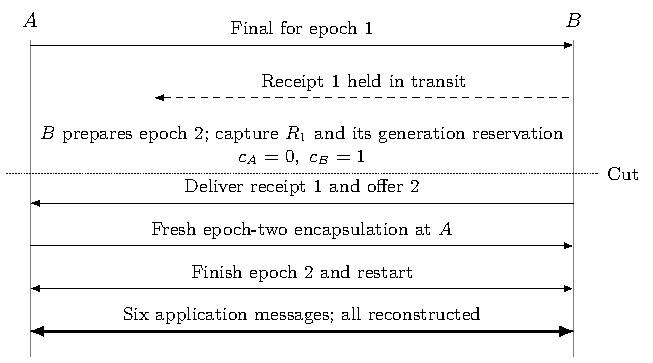
\includegraphics[width=\linewidth]{figures/confirmation-cut.pdf}
\caption{A retained native disclosure execution. The smaller confirmed counter
is zero at capture, while the captured reservation enables epoch-two traffic
recovery after the public exchange. The dotted Cut orders the exposure and the subsequent
fresh encapsulation; it does not refresh the earlier generation reservation.}
\label{fig:delayed-receipt}
\end{figure}

The resulting counterexample targets the proposed bound
$\min(c_A,c_B)+1$: its value is one, yet epoch-two traffic is exposed.
The protocol permits this asymmetric progress. Recovery reasoning therefore
follows the retained inputs and their descendants, with each endpoint's
confirmation counter retaining its own value.
% END SECTION SOURCE: construction.tex
% BEGIN SECTION SOURCE: security-model.tex
% This module uses amsmath, amssymb, amsthm, and the main document's
% definition, lemma, corollary, and proof environments.
% The normalization lemma below is a new, manually proved interface result.
% The separately cited Tamarin theorem is an existing symbolic result.

\section{Reservation origins, persistent records, and recovery}
\label{sec:security-model}

An interrupted cryptographic operation can retain its random tape before it
has produced a key or a ciphertext.  Its later execution and confirmation
therefore have to be related to the original reservation.  We make this
relationship explicit at two levels: the origin of a cryptographic operation,
and the origin of a saved session-state version.  A third identifier describes
the physical image that carries that version.  This distinction lets us
account for a target record copied by another session's write, an unapplied
pending image, and a ciphertext acquired before its wrapping key.

The model is an interface model for an asynchronous protocol machine
$\mathcal P$.  The adversary schedules public messages, process loss, honest
recovery, and the disclosure operations specified below.  Application
deliveries are private to the honest applications.  Capture grants read access
to the stated assets; it does not grant an additional operation for replacing
the authoritative journal.  An implementation with adversarial rollback or
forking requires those transitions in its storage machine.  The protocol,
its cryptographic primitives, and its public outputs are parameters of the
record-normalization lemma.  Fix finite execution, record-size, and query
budgets; the wrapper's bookkeeping is polynomial in their total
representation size.

Table~\ref{tab:record-notation} summarizes the principal objects.

\begin{table}[t]
\centering
\caption{Principal objects in the record model. The three identities separate
an original random draw, an immutable session-state version and its physical
storage representation.}
\label{tab:record-notation}
\small
\begin{tabularx}{\linewidth}{@{}>{\raggedright\arraybackslash}p{.25\linewidth}X@{}}
\toprule
Notation & Meaning\\
\midrule
$o,\rho_o$ & Original invocation and its reserved random tape\\
$v,X_v$ & Immutable session-state version and its payload\\
$h$ & Physical image or pending object carrying one or more versions\\
$\kappa$ & Identity of actual key material, shared by equal keys\\
$\mathsf{res}(o)$ & Event at which the original random tape is drawn\\
$\mathsf{save}(v)$ & First retention of $v$ on the durable acquisition surface\\
$\mathcal C_t,\mathcal L_t$ & Acquired and readable original versions at prefix $t$\\
\bottomrule
\end{tabularx}
\end{table}

\subsection{Three origins and their event order}

\begin{definition}[Reservation origin]
\label{def:reservation-origin}
A reservation origin is a fresh invocation index $o$, together with
\[
  \bigl(\mathsf{kind}_o,\mathsf{owner}_o,s_o,e_o,B_o,
        \mathsf{res}(o)\bigr).
\]
Here $\mathsf{kind}_o$ distinguishes generation, encapsulation, and any other
reserved operation; $s_o,e_o$ identify its session and epoch; $B_o$ is the full
canonical binding, including the admitted policy and operation inputs; and
$\mathsf{res}(o)$ is the event at which its random tape $\rho_o$ is drawn.
Execution or exact replay of $o$ consumes the same $\rho_o$ and the same
binding.  A new draw receives a new origin even if a failed attempt's external
operation identifier is reused.
\end{definition}

The ideal source in this model draws independent tapes of the prescribed
lengths.  Explicit entropy-disclosure queries reveal designated tapes.
Independence is a distributional assumption about the source at sampling.
Later API calls preserve the sampled tapes. The generation and encapsulation budgets
$G,C$ count original draws, including draws in attempts that subsequently
fail.  Exact retries consume no new slot.  Independently sampled operations
retain distinct origins even if some public outputs happen to coincide.

A record version $v$ has an immutable payload $X_v$ and semantic metadata
\[
  \bigl(\mathsf{subject}(v),\mathsf{role}(v),
         \mathsf{epoch}(v),\mathsf{phase}(v)\bigr).
\]
The subject identifies the session whose state is represented. A write to the
enclosing journal preserves this subject, including a write by another session.
A version can
refer to several reservation origins and to roots or traffic state derived
from earlier origins.  Preparing a version allocates its handle.  The event
$\mathsf{Saved}(v)$ occurs when that version first enters the durable
acquisition surface, and its time is denoted $\mathsf{save}(v)$.  In particular,
an intact target in a durable pending-write intent is saved before the
corresponding image is applied.  A storage operation may have made this
transition even when its caller receives an unknown-outcome error.

A physical object $h$ has a separate creation or sealing index.  It may carry
one version, several sessions' versions, an exact earlier image, or a pending
target.  An unchanged version keeps its $v$ and $\mathsf{save}(v)$ when it is
copied, archived, applied from a pending intent, or included in a newly sealed
aggregate.  A new semantic session-state version receives a new $v$ even when
some of its fields are unchanged.  These rules distinguish the original
reservation from each session-state update that retains it.

The following transition rules specify the provenance discipline.

\begin{enumerate}
  \item \emph{Reserve and execute.}  Reserve creates $o$ at the actual draw.
  Execution uses its retained binding and tape.  Unknown-outcome
  reconciliation keeps that origin; a definite new attempt allocates another.
  \item \emph{Prepare and retain.}  Preparing $v$ fixes $X_v$ and its provenance.
  Retaining the first intact image or pending target containing $v$ emits
  $\mathsf{Saved}(v)$.  An attempt that retains no such object has no successful
  acquisition event.
  \item \emph{Copy, apply, and reseal.}  An exact copy preserves the complete
  object and its sealing origin.  Resealing creates a new sealing invocation
  and its actual new wrapper randomness, while preserving the referenced
  record versions.  Applying an existing pending target copies its retained
  bytes.
  \item \emph{Crash and resume.}  Process loss removes volatile references.
  Recovery reconstructs the retained handles and their original provenance.
  It does not turn a retained reservation into a new draw.
  \item \emph{Confirm and delete.}  Confirmation changes protocol state and may
  authorize particular host-side deletions.  Neither action changes a
  reservation's origin or removes an adversary's previously acquired copy.
\end{enumerate}

For an original reservation actually retained in $v$, causality requires
\begin{equation}
  \mathsf{res}(o)\ \leq\ \mathsf{save}(v).
  \label{eq:origin-causality}
\end{equation}
A later physical object's creation time gives an additional timestamp, not a
replacement for either side of~\eqref{eq:origin-causality}.  The interval
between drawing $\rho_o$ and first retaining it remains explicit.  The
symbolic reservation-and-save transition can represent that interval only
through a separately justified source correspondence.

\subsection{Acquisition, delayed readability, and key identity}

Wrapping-key handles resolve to identities of actual key material.  Two
session labels that designate the same key resolve to the same identity
$\kappa$.  Disclosure through either label therefore enables every acquired
wrapper protected by $\kappa$.  A rotation creates a different identity when
it creates different key material.  Signing-key identities are treated in
the same way across sessions and roles.

For each intact physical object $h$, its construction records a finite set
\[
  \mathsf{paths}(h)=\{(v,\gamma)\},
\]
where $\gamma$ is the set of wrapping-key identities on a recoverable
serialization path to $X_v$.  Multiple paths to one version are permitted.
An unprotected record has $\gamma=\varnothing$.  Nesting a wrapper adds its
key identity; aggregation unions its members' paths.  An exact ciphertext
copy keeps its paths.  Resealing decoded records reconstructs the paths under
the new wrapper and retains the same $v$ values.  Thus resealing decoded
plaintext and wrapping an old ciphertext are distinct operations.

Only intact, recoverably embedded record payloads create these paths.  A
public hash or MAC of a private record is a public computation of that record,
not a path to the record itself.  The renderer introduced below preserves
that computation and its output.  This distinction prevents a public head
query from being relabeled as a snapshot merely because its computation used
private bytes.

\begin{definition}[Record acquisition and readability]
\label{def:record-acquisition}
A successful $\mathsf{Capture}(h)$ returns the actual retained bytes of $h$
and adds an immutable copy to the adversary's archive $\mathcal A_t$.
Let $\mathcal K_t$ be the wrapping-key identities disclosed by time $t$.
Define
\begin{align}
  \mathcal C_t
    &=\{v:\exists h\in\mathcal A_t,\ \exists\gamma,\
                    (v,\gamma)\in\mathsf{paths}(h)\}, \label{eq:acquired-records}\\
  \mathcal L_t
    &=\{v:\exists h\in\mathcal A_t,\ \exists\gamma,\
          (v,\gamma)\in\mathsf{paths}(h)
          \ \wedge\ \gamma\subseteq\mathcal K_t\}.
          \label{eq:readable-records}
\end{align}
Each capture records $\mathsf{AcquireOriginal}(v,t)$ for every version in its
support, including versions already acquired through another path.
An unsuccessful request for unavailable state returns its ordinary error and
adds no acquisition.
\end{definition}

Both sets describe the specified disclosure interfaces, using provenance and
key identities.  They do not test whether the adversary has guessed a secret.
The read set can grow without another capture: if $h$ was obtained at
$t_1$ and its final missing wrapping key is disclosed at $t_2>t_1$, the
corresponding versions enter $\mathcal L_{t_2}$.  Host deletion at an
intermediate time leaves $h$ in $\mathcal A_{t_2}$.  Acquisition, by contrast,
already occurred at $t_1$.

An additional key that is explicitly recoverable from an opened record can be
included by a declared extraction rule.  In this extension, iterate
\eqref{eq:readable-records} and the declared key-extraction rules to their least
fixed point after each event.  Each rule identifies its input bytes, its
deterministic extraction algorithm, and the resulting actual key identity.
Only rules with available inputs fire.  This accounts for nested protection
without assuming that inaccessible keys have already been learned.

Signer-file capture is a separately typed disclosure.  For correspondence
with the retained symbolic theorem, it records exposure of the actual signing
key conservatively at acquisition, as does that theorem's signer-file rule.
The readability ledger can additionally record when the file's contents
become decryptable.  In particular, a wrapping-key disclosure cannot be
scoped to traffic state when the declared capture also includes the matching
signer file.

\paragraph{Constructive exposure.}
From public protocol inputs, explicit leaks, and readable record payloads, we
form a labelled replay-dependency graph.  Its edges are specified algorithms:
unseal a reservation with its matching key; regenerate a key from its original
tape; replay encapsulation on the bound offer; decapsulate a published
ciphertext; derive a root; and derive the direction-specific traffic and ACK
material.  Directly stored roots, skipped keys, and plaintext enter through
their own record fields.  For the implemented root schedule, an edge is
\[
 (R_{e-1},S_e,C_e)\longmapsto
 R_e=\mathsf{HKDF}\bigl(R_{e-1},S_e,
       D_{\rm root}\Vert H_{\rm core}(C_e),32\bigr).
\]
Closing these explicit edges over the nodes of the bounded execution yields
a computable set of message keys with replay witnesses.  It supplies positive
exposure certificates; the
confidentiality game below is the separate criterion for messages outside
the declared disclosure conditions.  Confirmation counters belong to the
public progress state and do not reset this graph.

\subsection{An original-record implementation of the copy interface}

We now isolate a property of record management that is independent of KEM
secrecy.  The following two storage machines use the same protocol machine
$\mathcal P$, random-tape source, scheduler, and cryptographic interfaces.

The \emph{literal-copy machine} materializes the immutable payload $X_v$ in
each indicated serialization position.  Its objects include current images,
pending targets, and retained historical copies.  It records the origin tags
alongside these values as private bookkeeping.

The \emph{original-record machine} keeps one immutable table entry
$\mathcal O[v]=X_v$ and represents each serialization position by a reference
to $v$.  Its wrapper maintains the physical-object directory, pending states,
adversary archive, origin tags, and key identities.  It has the following
specified interfaces.

\begin{enumerate}
  \item $\mathsf{RegisterOriginal}(v,X_v)$ is a private write by the honest
  machine.  It fixes one value at a fresh $v$.  The wrapper receives the
  handle and the provenance metadata.
  \item $\mathsf{RenderOriginal}(\theta)$ evaluates the supplied serialization
  recipe $\theta$ by dereferencing $\mathcal O$.  A recipe specifies literal
  public fields, record references, references to already rendered objects,
  and each sealing, hash, MAC, or other admitted byte-processing call.
  A fresh sealing call uses a fresh invocation index and the same prescribed
  coin distribution as the literal-copy machine.  An exact-object read or
  replay returns its cached original bytes.
  \item $\mathsf{AcquireOriginal}(v,t)$ records acquisition of that version.
  This is an event, not an assertion of decryption.  A capture's externally
  returned bytes come from the rendered object cache.
  \item $\mathsf{RevealOriginal}(v)$ returns the original payload $X_v$.
  The wrapper uses this interface for a plaintext record-opening response
  only after a captured path is enabled by the disclosed keys, and caches
  the answer for subsequent openings.
\end{enumerate}

The renderer is an explicit trusted interface in this intermediate
experiment.  It has access to the original payload table and evaluates the
stated byte operations, including operations on undisclosed payloads.
Consequently, it can produce real ciphertexts, commitment digests, and report
MACs.  This definition does not supply an algorithm for producing those bytes
from an unknown KEM-challenge tape.  It gives a precise location for the
subsequent cryptographic replacement of that interface.

The operational contract has three further requirements.
First, all publicly visible payload-dependent bytes and statuses are obtained
through the specified renderer or through $\mathcal P$'s common protocol
computation.  Memory addresses and host timing are not additional outputs of
this interface.
Second, actual byte-operation order, error responses, partial transaction
outcomes, and cryptographic-oracle calls are retained.  Caching an exact
object does not discard a native hash-validation call, observable retry, or
write attempt: such an action remains a renderer or protocol action.
Third, the reference metadata and the key-identity relation are available to
the wrapper without inspecting a selected hidden reservation's coins.
These are checkable interface conditions; none asserts the secrecy of a
record, a root, or a message.

\begin{lemma}[Alias normalization]
\label{lem:alias-normalization}
For the operations and renderer contract above, every adversary
$\mathcal A$ interacting with the literal-copy machine has an online wrapper
$\mathcal B$ interacting with the original-record machine such that their
public views have the same distribution.  Their reservation-origin ledgers,
record-save events, acquisition events, and read sets are identical after
projection onto the original handles.

The wrapper makes at most $|\mathcal L_T|$ distinct
$\mathsf{RevealOriginal}$ calls by terminal time $T$.  Repeated physical
copies, captures, and openings do not multiply this number.  The wrapper
preserves every original reservation and every fresh sealing invocation, so
it does not merge their respective cryptographic resource counts.

The statement also holds for an adversary with quantum private state and
quantum access to common public cryptographic oracles, provided the storage
interface is classical and both experiments retain the same oracle calls.
\end{lemma}

\begin{proof}
Maintain a map from every literal record occurrence to its immutable handle
$v$, and from every native object identifier to a rendered-object entry.
Couple the protocol random tapes, sealing coins, scheduler choices, and public
cryptographic oracles between the experiments.  The invariant is that
dereferencing every original-record recipe produces the corresponding
literal-copy bytes, with the same semantic provenance and physical
disposition.

For a new record, register its payload once and extend the occurrence map.
For a fresh rendering, submit the same recipe and byte-operation sequence to
$\mathsf{RenderOriginal}$.  Dereferencing gives the same inputs to every
sealing, digest, MAC, validation, and output operation.  Coupled coins and
common oracles therefore give the same bytes, statuses, and state changes.
This step retains a write that became durable before returning an error;
the caller's status does not overwrite the persistence state.

An exact copy or pending-target application copies the object reference and
its original cache entry.  Aggregation collects the corresponding original
references, and resealing evaluates the new recipe using those references.
Each operation preserves the session-record handles and their save times.
It follows by induction on the recipe constructors that
$\mathsf{paths}(h)$ is the same in both machines.  A public hash or MAC
constructor contributes its common output and has an empty record-acquisition
path set.

On successful capture, output the cached object bytes in both experiments
and append its immutable descriptor to the adversary archive.  For each
version in its support, emit the same acquisition event at the actual
capture time.  Preserve the ordinary error for an unavailable object.
When a matching wrapping key is disclosed, use the common key identity and
reevaluate the enabled paths in the complete adversary archive.  For an
opening response, obtain $X_v$ from $\mathsf{RevealOriginal}$ on its first
use and from the wrapper's cache thereafter.  Every such call has
$v\in\mathcal L_T$.  Shared-key aliases and later key acquisition are thus
handled without another copy of $X_v$.  The optional key-extraction extension
preserves the invariant by induction on the least-fixed-point rounds.

Host deletion removes only host references.  The adversary archive and
already returned payloads persist.  Crash and resume use the same retained
object identifiers; neither operation recreates a reservation or changes a
save event.  Ordinary protocol actions are performed by the same
$\mathcal P$ with the same results.  This completes the induction, including
adaptive choices based on any preceding response.

For quantum private state, identical classical responses and the same public
oracle transformations induce the same transformation of that state at
each interaction.  The argument introduces no measurement of a quantum
oracle query and no oracle-dependent advice.  Finally, caching each
plaintext opening by $v$ proves the query bound; reservation and fresh-seal
indices were preserved separately throughout.
\end{proof}

The lemma places multiplicity in the correct ledger.  An adversary may retain
many ciphertext aliases of one version, and those ciphertexts may have many
different public heads.  All such byte-level observations remain in the view.
The repeated payload uses one original-record opening, whereas each genuinely
fresh seal and each public hash or MAC computation keeps its own resource
accounting.

% BEGIN SECTION SOURCE: guarded-provenance.tex
% Manuscript fragment. Requires amsmath, amssymb, amsthm.
\subsection{Explicit guarded normalization of record readability}
\label{sec:guarded-provenance}

The path and readability definitions above already account for copying and
later key disclosure. We now give their explicit guarded normalization and
an executable realization for a record-decryption specialization. Here key
derivation has fixed public edges independent of recovered plaintext. The
optional plaintext-dependent key-extraction extension remains as defined
above and is outside this specialization. The set $\Omega_{\rm src}$ below
contains reservation-source identities; it is distinct from saved record
versions and from the original-payload table $\mathcal O[v]$. Likewise,
$\mathcal E^{\rm src}_t$ projects derivability onto protected source values,
whereas $\mathcal C_t$ and $\mathcal L_t$ track acquired and readable versions.
The graph is a fixed representation of admitted retained objects, not a
replacement for the provenance transition rules or the byte renderer.


A source identifier names one original sampling operation.  An acquisition
history records what the adversary obtains, including objects obtained at
different times.  These are distinct objects of the model: a copy preserves
the former, while an additional acquisition can change the latter.

\paragraph{Immutable record graph.}
Let $\mathcal R$ be a finite set of immutable encrypted record objects.
Each $r\in\mathcal R$ has a matching decryption-key identity $\kappa(r)$,
a set of embedded child records $\operatorname{child}(r)$, and a set
$\operatorname{orig}(r)$ of protected source values in its plaintext.
Containment is acyclic.  Record identities distinguish ciphertext objects;
source identities distinguish original sampling operations.  Several
records can contain the same source.  A rewrapped record has a new record
identity and may have a new key, while retaining its source identity.
Key identities are equivalence classes of equal actual keys. Equal key bytes
therefore have one identity across separate API objects.

Let $\mathcal D\subseteq\mathcal K\times\mathcal K$ be fixed public key
derivation edges.  An edge $(k,k')$ means that possession of $k$ permits
deterministic computation of $k'$.  This interface represents, for example,
derivation of an operation-wrapping key from the journal key.  In the
theorem below, these edges do not depend on plaintext recovered from records.
Write $D^*$ for their reflexive transitive closure.

Let $\Omega_{\rm src}=\bigcup_{r\in\mathcal R}\operatorname{orig}(r)$ be the
declared source domain.  At a trace prefix $t$, let $A_t\subseteq\mathcal R$ be all record objects
ever acquired by that prefix, $K_t\subseteq\mathcal K$ all directly
disclosed keys, and $\mathcal S^{\rm dir}_t\subseteq\Omega_{\rm src}$ all directly disclosed source values, represented
by their source identities.  These are cumulative sets.  The decryption-key
closure is
\[
  K_t^*=\{k':\exists k\in K_t,\ (k,k')\in D^*\}.
\]
The concrete derivation rules are
\[
 \frac{k\quad(k,k')\in\mathcal D}{k'},\qquad
 \frac{r\quad\kappa(r)}{c}\ (c\in\operatorname{child}(r)),\qquad
 \frac{r\quad\kappa(r)}{o}\ (o\in\operatorname{orig}(r)).
\]
Their least closure starts from $A_t,K_t,\mathcal S^{\rm dir}_t$.  A fact $o$ in the source
sort means that the protected value of source $o$ is derivable; it does
not mean that a public identifier has become known.  The source projection
of this closure is denoted $\mathcal E^{\rm src}_t$.

\paragraph{Guarded routes.}
For every path $p=(r_0,\ldots,r_\ell)$ in the containment graph ending
at a record with $o\in\operatorname{orig}(r_\ell)$, define
\[
 g(p)=\{\kappa(r_0),\ldots,\kappa(r_\ell)\}.
\]
The normalized table contains a route $(r_0,g(p),o,p)$ for every such
path.  Its exposure expression is
\[
 \widehat{\mathcal E}^{\rm src}_t=\mathcal S^{\rm dir}_t\ \cup\
 \{o:\exists(r,g,o,p),\ r\in A_t\ \land\ g\subseteq K_t^*\}.
 \tag{GP}
\]
Alternative records and paths are disjoined, while all keys on one path
are conjoined.  Equal key identities occur only once in the guard set.

\begin{theorem}[Exact guarded normalization]
\label{thm:guarded-normalization}
For every finite record graph and derivation interface above, and every
acquisition prefix $(A_t,K_t,\mathcal S^{\rm dir}_t)$, the concrete and normalized exposure
sets agree: $\mathcal E^{\rm src}_t=\widehat{\mathcal E}^{\rm src}_t$.  The equality applies to all prefixes of
an adaptively chosen history.
\end{theorem}
\begin{proof}
Key derivations depend only on disclosed keys and the fixed relation
$\mathcal D$, so their least closure is exactly $K_t^*$.
For the forward inclusion, take a source $o\in \mathcal E^{\rm src}_t$.
If it was directly disclosed then $o\in \mathcal S^{\rm dir}_t$.
Otherwise its first derivation decrypts a record $r_\ell$ with the
matching key.  If that record was not acquired directly, its first
availability follows by decrypting a parent.  Follow these first
derivations backwards.  The finite acyclic record graph makes this
process terminate at an acquired record $r_0$.  Every intervening key
lies in $K_t^*$, yielding a route satisfying (GP).
For the reverse inclusion, take a satisfied route.  Starting with its
acquired first record, successively decrypt along the path.  Every
required key is in $K_t^*$, so each child and finally $o$ is in the
concrete least closure.  Direct disclosures are in that closure by
definition.  Both inclusions hold for each fixed prefix; no independence
or advance choice of the acquisition schedule was used.
\end{proof}

\paragraph{Efficient evaluation.}
Equation (GP) is a declarative normal form: a compressed record DAG can
have exponentially many paths.  An efficient leakage evaluator instead
computes the iterative decryption and key-derivation fixed point, without
enumerating those paths.  Let $N$ be the total number of record, key and
source atoms, and let $M$ count rule and payload incidences.  There are at
most $N$ strict-growth rounds; repeated rule scans therefore take
$O(N(N+M))$ time and $O(N+M)$ space under standard indexed set and
dictionary representations, with source-dictionary operations included
in this accounting.  The finite checker materializes the route table only
for its declared small fixtures, to compare that normal form against the
forward evaluator.

\begin{corollary}[Copies, deletion and late disclosure]
\label{cor:guarded-history}
Exposure is monotone under additional acquisitions, direct disclosures
and key disclosures.  Copying or rewrapping a source adds routes to the
same source identity.  Local deletion of a record previously acquired
does not remove its routes from adversarial knowledge.  In particular,
a later matching-key disclosure can expose a source in a ciphertext
acquired before that disclosure and deleted locally in the meantime.
\end{corollary}
\begin{proof}
The cumulative sets and their key closure only grow, and every predicate
in (GP) is positive.  A source-preserving copy changes a route's record
identity or key guards but not its terminal source.  Local deletion
restricts future acquisition from that local store; it removes no member
of $A_t$ and therefore cannot invalidate a satisfied route.
\end{proof}

\paragraph{Interface significance.}
The theorem gives an exact finite normalization of the chosen
record-decryption semantics.  It supports a precise original-operation
leakage oracle: a query for source $o$ can be evaluated against the
complete acquisition history, with a path and its key guards as a witness.
The cryptographic transition from native ciphertexts and public
commitments to this interface has a separate simulation obligation.
The derivation rules do not model guessing, cryptanalysis, timing leakage
or a quantum decryption oracle.  Accordingly, absence from $\mathcal E^{\rm src}_t$ is
recorded as non-derivability by these rules; message indistinguishability
outside an exposure set is supplied by a security theorem for the
surrounding protocol.

\paragraph{Native shape and finite checks.}
At the fixed research source, operation reservations are encrypted under
a wrapping key derived from the journal key, and tokens are retained
within encrypted durable images or pending targets.  The corresponding
route therefore includes the image key and the token key, with their
actual derivation edge.  A fresh aggregate image can preserve an older
token and its original source.  Public image-head digests are distinct
observations from the record objects needed by the decryption rules.
The executable supplement independently evaluates iterative decryption
and guarded-route normalization, exhausts all acquisition/key/direct-source
subsets for its declared finite graphs, and checks histories with late
key disclosure and local deletion.  Its counts and source hash are in
the accompanying machine-readable result; those checks validate the
implemented finite model and supplement the general proof above.
% END SECTION SOURCE: guarded-provenance.tex
% BEGIN SECTION SOURCE: acquisition-nonadditivity.tex
% Standalone manuscript fragment; no preamble.
% Requires proposition and proof environments (e.g. amsthm).
\paragraph{Why exposure must retain conjunctive guards.}
The following elementary separation explains the conjunction in (GP).

\begin{proposition}[Acquisition exposure is not additive]
\label{prop:acquisition-nonadditivity}
Let $r$ be a retained-record atom, $k$ a wrapping-key atom, and $s$ a
protected-seed atom associated with an origin identifier $o$.
For $A\subseteq\{r,k\}$, let $\operatorname{Cl}(A)$ be the least set
containing $A$ and closed under the rule
\[
  \{r,k\}\;\Longrightarrow\;s.
\]
There are no other rules in this fragment.  Define the exposed-origin set by
\[
  E(A)=\{\,o : s\in\operatorname{Cl}(A)\,\}.
\]
There is no fixed function
$f:\{r,k\}\longrightarrow\mathcal{P}(\{o\})$ satisfying
\[
  E(A)=\bigcup_{x\in A} f(x)
  \qquad\text{for every }A\subseteq\{r,k\}.
\]
\end{proposition}

\begin{proof}
The closure rule gives
\[
  E(\{r\})=E(\{k\})=\varnothing,
  \qquad
  E(\{r,k\})=\{o\}.
\]
Exactness for the two singleton acquisitions forces
$f(r)=f(k)=\varnothing$.  Their union is then empty for the joint
acquisition, contradicting $E(\{r,k\})=\{o\}$.
\end{proof}

\paragraph{Meaning of exposure.}
The proposition concerns derivability in an explicitly specified rule
system.  The identifier $o$ may itself be public; its membership in $E(A)$
records derivability of its protected seed, not discovery of the identifier.
Derivability excludes guessing and is not a claim that a computational
adversary has zero success probability.  As a separate probabilistic
illustration, let $S,W$ be independent uniform $\lambda$-bit strings and
$C=S\mathbin{\oplus}W$, with no additional observation depending on $S$ or
$W$.  Then
\[
  H(S\mid C)=H(S\mid W)=\lambda,
  \qquad H(S\mid C,W)=0.
\]
From either observation alone, any estimator of $S$ succeeds with
probability at most $2^{-\lambda}$; from both, $S=C\mathbin{\oplus}W$
recovers it exactly.  This illustration does not instantiate the record
encryption used by the protocol.

\paragraph{Consequence for provenance routes.}
A source label and an exposure decision serve different purposes.  Copying
a retained record preserves the source label, while subsequent acquisition
of a matching key may change exposure.  A guarded-route representation
retains this distinction: alternative acquired records supply alternative
routes to the same source, and every route retains the conjunction of its
required keys.  Exposure is therefore evaluated from the joint acquisition
and key-derivation history.  The proposition does not rule out stateful
labels, history-dependent vulnerability sets, or conservative per-object
overapproximations; it rules out an exact, fixed, per-object union in the
presence of the stated conjunctive dependency.
% END SECTION SOURCE: acquisition-nonadditivity.tex

\subsection{A recovery experiment with acquisition-based eligibility}

\begin{definition}[Fixed-target recovery experiment]
\label{def:recovery-game}
Fix a protocol profile $\mathcal P$ and finite execution budgets, together with
a designated session $s$, recovery cut $c$, target epoch $e$, and candidate
generation and encapsulation reservation handles $g_e,a_e$.  Handles may be
named by original invocation slots before those invocations occur; a missing
invocation will fail the reservation-event test below.  Public
protocol messages may be delayed, duplicated, reordered, or replaced.
The adversary can capture the declared retained objects, reveal wrapping
keys, reveal actual signing keys or signer files, and reveal designated
reservation tapes.  The cut exposes the selected wrapping keys; preceding
roots may already be public or disclosed by the stated prior captures.
These disclosures have their exact scope in the event ledger.

For one fresh logical application send, the adversary supplies equal-length
messages $(m_0,m_1)$.  The challenger samples $b\leftarrow\{0,1\}$ and runs
the ordinary sending transition on $m_b$.  Rejection or an unknown outcome
keeps its ordinary protocol behavior.  A retained accepted send is identified
by $(s,e,d,j)$, including direction $d$ and the epoch-scoped logical index $j$;
exact retries reuse its original ciphertext.  The challenge is valid only
when that logical send is accepted in the designated epoch.  Subsequent
protocol actions and disclosures continue until the adversary outputs $b'$.
\end{definition}

Write $\iota_A,\iota_B$ for the two actual signing-key identities configured
for the target session.  The predicate
$\mathsf{ReservedFor}(s,e,g_e,a_e)$ checks the occurrence of the named honest
generation and encapsulation reservation events in the target epoch's local
durable plans, with their target session and roles.  It checks event metadata,
without asserting that their outputs form the accepted target exchange.
Eligibility uses the following event conditions over the complete execution:
\begin{align}
 \mathsf{Eligible}_{s,e,c}(\tau)\ \Longleftrightarrow\quad&
 \mathsf{ValidTarget}(\tau)
 \ \wedge\ \mathsf{ReservedFor}(s,e,g_e,a_e)
 \nonumber\\[-1mm]
 &{}\wedge\ c<\mathsf{res}(g_e)
          \ \wedge\ c<\mathsf{res}(a_e)
 \nonumber\\
 &{}\wedge\ \iota_A,\iota_B
                  \notin\mathsf{IdentityExposed}(\tau)
 \nonumber\\
 &{}\wedge\ \mathsf{EntropyExposed}(s,e;\tau)=\varnothing
 \nonumber\\
 &{}\wedge\ \nexists v\in\mathcal C_T:
       \mathsf{subject}(v)=s\ \wedge\ c<\mathsf{save}(v).
 \label{eq:eligibility}
\end{align}
Here $\mathsf{EntropyExposed}(s,e;\tau)$ records the target epoch's designated
entropy disclosures.  The separate event $\mathsf{Attr}$ states that these
named reservation events form the accepted target's unique usable
generation/encapsulation pair, with an adapter-computable association to the
original slots.  In particular, it connects the generation public key, the
encapsulation input, the authenticated response, and the target's subsequent
key schedule.  This matching is a
source/authentication obligation: a failure of $\mathsf{Attr}$ can occur while
$\mathsf{Eligible}_{s,e,c}$ holds and is charged in the computational
accounting.

The final line of~\eqref{eq:eligibility} concerns every saved version of session
$s$, across its roles and epochs.  It uses acquisition
$\mathcal C_T$, including protected bytes, at the time they are obtained.
Readability $\mathcal L_T$ is evaluated separately. Other epochs' entropy disclosures retain their ordinary
behavior.  Both peers' confirmation is not an additional send prerequisite.

Define the unconditional centered advantage by
\begin{equation}
 \mathsf{Adv}^{\rm rec}_{\mathcal P}(\mathcal A)
   =
 \left|
   \mathbb E\!\left[
    \mathbf 1_{\mathsf{Eligible}_{s,e,c}(\tau)}
                       (-1)^{b\oplus b'}\right]
 \right|.
 \label{eq:recovery-score}
\end{equation}
Invalid or ineligible executions contribute zero.  This definition retains
failures and adaptive disclosures in the probability space and avoids
conditioning a reduction on an uncontrolled eligibility probability.
If every execution with $\mathsf{Eligible}_{s,e,c}=0$ is completed by an
independent fair guess, the conventional advantage over one half is
\[
 \mathsf{Adv}_{\rm msg}
   =\left|\Pr[\text{completed guess is correct}]-\tfrac12\right|
   =\tfrac12\,\mathsf{Adv}^{\rm rec}_{\mathcal P}(\mathcal A).
\]
The computational accounting uses this latter convention.

The adaptive version retains one application challenge and permits the
candidate selector to choose its coordinates and reservation-event handles
adaptively from the observed interaction. Eligibility
requires those coordinates to identify the challenge's accepted logical send;
selection never transfers its test bit to another send.  Eligibility
and the usable-pair attribution are evaluated on that experiment's complete
history.  An origin-pair reduction fixes a slot pair in $[G]\times[C]$ and
scores the event that the final selector attributes the target to that pair.
The selector and disclosure predicates are recomputed in each comparison
world.  No independence between that selection and the transcript is imposed.

The record restriction in~\eqref{eq:eligibility} is the one used by the
retained multi-epoch symbolic theorem: its \textsf{Snapshot} action outputs
a protected record, while \textsf{Cut} separately releases the wrapping keys.
The theorem establishes symbolic plaintext secrecy with both original
reservations after the cut, key-scoped identity exclusions, the target
entropy exclusion, and the stated post-cut saved-record acquisition
exclusion~\cite{qperiaptSymbolic2026}.  Its joint replay verifies the main
lemma and all 24 reusable dependencies.  Equation~\eqref{eq:recovery-score}
specifies the computational message experiment to which the cryptographic
modules are to be connected; the alias lemma establishes its record-interface
normalization.

\begin{corollary}[Safe stopping at a forbidden acquisition]
\label{cor:target-acquisition-stop}
Consider the fixed-target experiment of
Definition~\ref{def:recovery-game}.  Suppose an actual successful capture
contains a target-session version $v$ with $c<\mathsf{save}(v)$, identified
by the original-record metadata.  For any terminal bit $D$, replacing the
remainder of that execution by output zero leaves
\[
   \Pr[\mathsf{Eligible}_{s,e,c}(\tau)\wedge D=1]
\]
unchanged.  Replacing its terminal score by zero also leaves the expectation
inside~\eqref{eq:recovery-score} unchanged.

In particular, if a captured target-session version retains the selected
reservation $o\in\{g_e,a_e\}$, then
$c<\mathsf{res}(o)$ and~\eqref{eq:origin-causality} establish this stopping
condition.  The wrapping key may be obtained before or after the capture.
\end{corollary}

\begin{proof}
The successful capture inserts $v$ into $\mathcal C_t$ immediately.
Its save time and subject are immutable, and acquisition remains recorded
after host deletion, resealing, confirmation, or process loss.  Thus the
last conjunct of~\eqref{eq:eligibility} is false for every continuation.
Each such continuation already contributes zero to both quantities.
On executions that never reach this condition, the experiment is unchanged.
The final assertion follows from
$c<\mathsf{res}(o)\leq\mathsf{save}(v)$.
\end{proof}

The stopping test uses the successful acquisition event and its record
metadata; it can run before the response's private bytes are serialized by
a challenge adapter.  It is not an SDK rejection of the capture.  A public
digest, an unrelated record, or an unsuccessful capture keeps its real
behavior.  In particular, difficulty computing a permitted digest or report
MAC does not trigger this corollary.
For adaptive target selection, stopping is applied to the corresponding
fixed-candidate event in the reduction.  One possible candidate becoming
ineligible does not justify terminating a game that can still select a
different eligible target.

Two short executions illustrate why both kinds of origin are necessary.
If $v$ was saved before $c$ and a sibling write reseals it after $c$, the
acquisition still refers to the original pre-cut $v$.  The new global image
time alone does not falsify the final conjunct of~\eqref{eq:eligibility}.
If instead $v$ was saved after $c$, a later write attributed to a sibling
does not change its subject or make its capture eligible.  Likewise, a
pre-cut generation reservation retained through a delayed receipt remains
pre-cut when its KEM computation completes later. The reservation condition
in~\eqref{eq:eligibility} determines that case, with the endpoints retaining
their respective confirmed counters.

\subsection{Connection to the cryptographic argument}

The normalization theorem fixes the original objects whose bytes, acquisition,
and key identities the reduction must represent. The next section gives
constructive image/intent and report interfaces for a selected KEM operation
whose public outputs are available while its original random tape is opaque.
Their algorithms preserve original-object caches, public commitments, exact
retries, and actual durable outcomes. The fixed-target stopping rule above
extends to an adaptive provenance certificate in
Lemma~\ref{lem:adaptive-origin-stop}.

Usable attribution is computed from available semantic metadata. Original
generation and encapsulation slots belong to a fixed lifetime budget
$[G]\times[C]$: a fresh draw receives a new slot, while copies retain their
source. Each candidate induces its own protected records and report-key
closure. Proposition~\ref{prop:native-local-accounting} decomposes the score
in the native experiment before comparing those local continuations. It
retains both unattributable eligible executions and permitted key projections
as explicit native-game terms.

The computational composition evaluates accepted operations, eligibility, and
all public outputs anew in each comparison world. Exact component repeats
retain one response and one correctness event. The native constructor map in
Section~\ref{sec:native-correspondence} identifies the storage operations used
by these interfaces; Section~\ref{sec:discussion} specifies the joint root and
message continuation to which their bounds connect.
% END SECTION SOURCE: security-model.tex
% BEGIN SECTION SOURCE: computational-roadmap.tex
\section{Computational interfaces and composition}
\label{sec:computation}

The origin model provides the accounting boundary for a computational
experiment. Each original generation or encapsulation invocation receives a
slot when its entropy is reserved, including attempts that later fail.
Replaying or copying that reservation retains its slot. Fix public lifetime
budgets $G,C\geq1$ and write $J=[G]\times[C]$. Unused slots remain unused.
These proof-resource budgets differ from a bound on the number of records
resident at one time.

The native application experiment evaluates the selected target after the
adversary's interaction. Eligibility requires both original reservations to
follow the selected cut, secrecy of the actual target signing keys and
target-epoch entropy, and no acquisition of a selected-session version saved
after that cut. It admits the asynchronous transitions of the construction,
including sending after the local FinalReady transition.

We first construct the private-record and immutable-report interfaces. We
then connect their candidate-specific continuations to one native score,
using original provenance to certify permanent local stopping. After the
native constructor correspondence, a joint key-schedule theorem derives the
selected first-message continuation from a uniform recovered contribution.
The common-virtual-game
accounting variant is retained in Appendix~\ref{app:common-virtual}.

% BEGIN SECTION SOURCE: opaque-rendering.tex
\subsection{An explicit renderer for private images and intents}
\label{sec:opaque-rendering}

The alias lemma preserves a renderer that can read every original payload.
A component reduction additionally needs to execute record management when
the selected KEM challenger supplies public outputs and a shared-secret
challenge without supplying the selected random tape. We construct that
record-management algorithm for a finite image/intent interface. Its tables
contain immutable handles, known fields and locally sampled sealing coins.
The protocol's public computations are supplied by a common functional
interface $F$, instantiated by the original-operation adapter. This section
holds $F$ fixed and isolates the image/intent contribution to the record
connection in Proposition~\ref{prop:native-local-accounting}.

\paragraph{Typed record interface.}
An opaque block is an immutable fixed-length private value, represented by a
handle and its known length. Blocks may be correlated and may themselves be
retained sealed reservations. A private image recipe contains at least one
such block; an atom-free recipe is fully known. Local image-encryption and
intent-authentication keys are available to the simulator. Fix a public
budget $M$ for all fresh image-sealing invocations, including failed attempts
and atom-free images. Exact copies and exact retries retain their invocation.
The following operations specify the interface.

\begin{enumerate}
  \item \emph{Seal.} Before sampling its nonce, invocation $i$ fixes the
  recipe, its length and the non-nonce header fields. It samples independent
  $N_i\gets\{0,1\}^{n}$ and privately constructs
  \[
    B_i=\mathsf{Hdr}_i\Vert N_i\Vert C_i,
  \]
  where $C_i$ is the specified deterministic local authenticated encryption
  under that nonce. Local encryption and intent authentication use their
  prescribed fixed algorithms without additional shared-SHA3 calls. All
  admitted image formats place the nonce at the same offset. The reply
  consists of the image handle, length and declared non-nonce metadata;
  $N_i$, $C_i$ and the recipe's private blocks remain private.
  \item \emph{Intent.} A complete canonical prefix $P$ fixes the tag,
  binding, predecessor and the image-head value used in this execution.
  Its tag determines its length. The intent bytes are
  \[
    W_{i,P}=P\Vert B_i\Vert
       \mathsf{MAC}_{k_i}(P\Vert B_i),
  \]
  with one fixed authentication key $k_i$ for image $i$. An exact repeat
  retains the same $(i,P)$ entry. Image and intent tags are disjoint.
  \item \emph{Public commitments.} For a designated private image, the
  ideal-commitment experiment returns independent uniform 256-bit values
  cached by $i$ for its head and by $(d,i,P)$ for its intent digests. The
  domain $d$ ranges over the five admitted intent-digest domains. Atom-free
  objects retain their real hashes and ordinary raw-byte outputs. Later
  validation and zero-value checks use the actual replies in that execution.
  \item \emph{Equality and storage.} Equality queries compare complete
  retained image or intent handles. Copy, retain, persist, delete, crash
  and resume update an explicit durable-state directory. Storage choices,
  errors and branch decisions depend on available metadata, lengths,
  commitments and $F$ outputs. A failure after commit preserves that commit.
  \item \emph{Acquisition.} Atom-free objects are rendered from their known
  inputs. For an opaque object, the admitted successful acquisition emits
  a computable event that permanently falsifies the fixed-candidate
  eligibility before its raw bytes are returned. The stopped score is zero,
  as in Corollary~\ref{cor:target-acquisition-stop}. Unavailable-object requests
  retain their ordinary error result.
\end{enumerate}

All other public computation uses these replies, known inputs, $F$, and the
shared public oracles. This is a classical record interface; the adversary
may have quantum private state and quantum access to those public oracles.
The successful-acquisition condition is supplied by the recovery experiment's
existing event rule. For a fixed target session $s$ and cut $c$, acquisition
of an original version $v$ with $\mathsf{subject}(v)=s$ and
$c<\mathsf{save}(v)$ supplies such an event. Its original-record provenance
determines that save time, including when a later aggregate carries the same
version. Lemma~\ref{lem:adaptive-origin-stop} gives a provenance certificate
valid before the final cut is chosen. A separately permitted projection is
described by its own output operation.

\paragraph{Table algorithm.}
The simulator stores an image table indexed by fresh sealing invocation,
an intent table indexed by image and complete prefix, a commitment cache,
and the directory with its provenance and acquisition ledgers. Each new
image entry records the recipe handles, length, known fields and a sampled
nonce. Each new intent entry records $(i,P)$ and its known length. The
simulator samples designated-private commitments on first use and retrieves
them on exact retry; it constructs and hashes atom-free objects normally.
Equality is structural: images compare equal exactly when their indices
match, and intents compare equal exactly when their pairs $(i,P)$ match.
The storage directory determines the state recovered after a crash, including
an acknowledged or uncertain write that actually committed. At the stipulated
permanent-failure acquisition event the computation returns zero. Every other
transition executes the common public code and $F$. Thus the algorithm uses
no selected opaque block bytes.

\begin{lemma}[Structural equality of complete records]
\label{lem:record-structural-equality}
If the nonces of fresh image invocations are pairwise distinct, then
\[
 B_i=B_j\iff i=j,\qquad
 W_{i,P}=W_{j,P'}\iff(i,P)=(j,P').
\]
\end{lemma}
\begin{proof}
One immutable image handle retains one byte string. Two different image
invocations have different nonces at the same explicit offset, so their
complete wires differ. Intent tags first separate different formats. For
one tag the prefix length is fixed: unequal prefixes differ before the
target image, while equal prefixes with different images differ at the
target's nonce. The same image and prefix give the same deterministic MAC
under the fixed key. Disjoint tags also separate images from intents.
This argument permits coincident private block values and ciphertext
components; the explicit nonces distinguish the complete images.
\end{proof}

Let $I$ be the materialized ideal-commitment experiment, which retains real
private bytes and answers equality by comparing them. Let $T$ be the table
algorithm above. Both use the stipulated fixed-candidate stopping rule and
the same public-oracle model and interface $F$.

\begin{theorem}[Opaque image/intent simulation]
\label{thm:opaque-rendering}
For at most $M$ fresh seals with independent $n$-bit nonces, define
\[
 \delta_{\rm nonce}=\min\{1,\tbinom M2\,2^{-n}\}.
\]
For every efficient terminal bit $D$ computed from the public view, available
metadata and event ledger, $F$ outputs and its own independent test coins
(including its retained application challenge bit),
\[
  |\Pr[I:D=1]-\Pr[T:D=1]|\leq\delta_{\rm nonce}.
\]
For a score $Z\in[-1,1]$ computed from the same available inputs,
$|\mathbb E_I Z-\mathbb E_T Z|\leq2\delta_{\rm nonce}$.
\end{theorem}
\begin{proof}
Couple the fresh sealing nonces, private-commitment replies, scheduler choices,
the state of $F$, and the public-oracle transformations. Before the first
nonce collision, maintain agreement of the directories, known fields,
immutable references, public bytes, statuses and semantic ledgers.
Sealing adds the same metadata and nonce to corresponding entries; its
private ciphertext is confined to the materialized entry. Intent creation
adds the same complete prefix and target reference. A fresh private
commitment gets the coupled reply, and a repeat consults the same cache.
Atom-free commitments and acquisitions use identical materialized inputs.
Lemma~\ref{lem:record-structural-equality} gives agreement of equality replies.
The common public computation consequently makes the same transitions and
oracle calls. Copying, committed or failed writes, deletion, crash and
resume preserve the directory invariant. An opaque acquisition emits the
same permanent-failure event before either computation needs to return its
unknown bytes, and both stopped scores are zero.

The next nonce is independent uniform even when the decision to seal is
adaptive. Across at most $M$ invocations, a union bound charges
$\binom M2 2^{-n}$ for any collision. Coupled terminal bits differ only on
that event; bounded scores can differ by at most two. Identical classical
replies and shared-oracle transformations also preserve a quantum
adversary's state at every coupled good prefix. The argument uses no
measurement of a quantum query.
\end{proof}

\paragraph{Connecting real commitments.}
After replacing complete-wire equality by structural equality, let
$\epsilon_{\rm com}$ bound the bit-distinguishing gap between real private
record digests and the independently cached commitments of the typed
interface. Both games run the same public code, ordinary known-record
computations, available metadata and declared stopping rule. The comparison
counts the full distinguishing computation against their shared public oracle.
It is a cryptographic input to the following composition, separate from the
explicit table simulation. Appendix~\ref{app:primitive-inputs} records the
concrete multi-record bound under fixed-input injectivity, per-nonce
confinement and the prescribed local encryption/authentication algorithms.

\begin{corollary}[Real-record to table-algorithm bound]
\label{cor:real-to-opaque}
For the declared fixed-candidate interface and the commitment conditions
above, let $R$ be the real-digest materialized experiment. With $n=192$,
\[
 |\Pr[R:D=1]-\Pr[T:D=1]|
 \leq\min\{1,\epsilon_{\rm com}+\delta_{\rm nonce}\}.
\]
The corresponding $[-1,1]$ score bound is
$\min\{2,2(\epsilon_{\rm com}+\delta_{\rm nonce})\}$.
When the interface exposes no private-wire equality query, its additional
$\delta_{\rm nonce}$ term is zero.
\end{corollary}
\begin{proof}
First replace real byte equality by structural equality, coupling exactly
as above and charging $\delta_{\rm nonce}$. The resulting game has no extra
nonce-dependent equality observation, so apply the stated private-commitment
replacement there. Its ideal form is implemented exactly by the table
algorithm. A triangle inequality proves the bit bound. Applying that bound
to a test that returns one with probability $(1+Z)/2$ proves the score bound.
Without a private-wire equality operation the first replacement is absent.
\end{proof}

The hybrid order starts with constructible real record inputs, replaces
their private commitments, and then uses the table algorithm for the KEM
challenge embedding. Every changed commitment is consumed by that world's
subsequent intent prefixes, checks and outputs. For an adaptive origin-pair
event $E_j$, early stopping is justified only by a computable event making
$E_j$ false for every continuation and every still-admissible final target
choice attributed to $j$. The disjoint-event accounting above retains this
per-pair obligation.
% END SECTION SOURCE: opaque-rendering.tex
% BEGIN SECTION SOURCE: report-composition.tex
% Independent module; no changes to the frozen manuscript.
% Source: multi_report_theorem.md, reverse-order report composition.
\subsection{Immutable report families and reverse-order composition}
\label{sec:report-composition}

A later cleanup report can authenticate an earlier report's private key and
tag.  We compose the one-report HMAC replacement by creation order, retaining
these dependencies.  The reduction below supplies a concrete algorithm for
handling a selected unknown report key: later dependent rows are already ideal,
and earlier immutable transcripts precede that key.

\paragraph{Finite interface.}
Fix a public budget $N$ for fresh report-key draws and index the actual draws
chronologically.  Failed attempts retain their indices; a new draw after
definite absence receives a new index.  Exact replay of a retained original
report keeps its index, key, and transcript.  Each $K_i$ is an independent
uniform 256-bit value, with no rejection of the zero key.

Let $\mathcal X$ be the source-atom handles whose bytes the subsequent KEM
adapter will not possess.  In this report replacement, their real bytes are
still available to the surrounding source experiment.  Before using $K_i$, the
machine fixes a bounded immutable transcript recipe $m_i$.  It can contain
available literals and protocol outputs, atoms in $\mathcal X$, earlier raw
keys $K_j$ with $j<i$, and previously returned tags.  Its own key and tag do not
occur in $m_i$.  Lengths, dependency sets, and admission errors are computable
from the recipe metadata.  Native code may draw the key before assembling the
transcript, preserving that order and its failures, provided those inputs do
not depend on the draw.  Every direct or computed use of a raw key retains its
origin dependency; returned tag bytes are available values.

Compute an online protection flag before using the fresh key:
\begin{equation}
 P_i=\mathbf 1\!\left[
 \operatorname{deps}_{\mathcal X}(m_i)\ne\varnothing
 \;\lor\;
 \exists j<i:\ P_j=1\ \land\ K_j\in\operatorname{deps}_{K}(m_i)
 \right].
 \label{eq:report-protection}
\end{equation}
This is forward closure under raw-key dependencies.  It need not propagate
through a previously returned tag.  The flag uses origin references, not
actual key equality or the primitive challenger's bit, and is recomputed in
each comparison world's history.

The following operations specify the interface.  Creation computes
$t_i=\operatorname{HMAC}_h(K_i,m_i)$ and retains the actual nonzero-ID check,
encoding errors, and persistence outcomes.  Replay or validation names the
original report and uses that same $m_i$; supplied identifiers can be compared
with its retained tag.  This operation does not submit changed private bytes
as a new transcript under $K_i$.  Acknowledgement, terminal-tag comparison,
copying, and crash recovery preserve their ordinary original-handle semantics.
Private storage uses the explicit recipe tables of the opaque-record
interface, including its already idealized commitments and its separate error
accounting.  Public report bodies and other outputs use available inputs or
their specified application interface.  Protected raw keys have no additional
unlisted computation or observation channel.

The full real experiment $G$ retains each declared fragment/key disclosure.
Let $\mathsf{Bad}_{\rm rep}$ be the first successful outward projection whose
recipe depends on a raw $K_i$ with $P_i=1$, detected by its actual origin map
before returning the dependent bytes.  An unavailable fragment, a terminal
tag alone, or a projection without that dependency does not trigger it.
Define $G^{\rm stop}$ to end with score zero at this event.  This is an
analysis game; a report-key fragment is not thereby declared to be a
selected-session acquisition or a new freshness failure.

\paragraph{One-row bound and hybrids.}
Use one public compression oracle $h$ for all rows and quantum queries.
The one-row experiment draws a uniform hidden 256-bit key $K$, independently
of $h$ and oracle-independent initial auxiliary state. The algorithm performs
its complete counted preparation and chooses one classical transcript $m$ of
length at most $L$ without a raw-key input. Its first row query returns either
$\operatorname{HMAC}_h(K,m)$ or an independent uniform 256-bit tag; at most
$T\ge1$ row calls repeat this same transcript and cached answer. The algorithm
has no additional raw-key, midstate or key-dependent output interface.
It may continue querying the same $h$ and output a bit. The budget $q$ counts
all public compression queries, including preparation, other real rows,
continuation and the terminal test. Independently sampled known keys may
coincide with $K$; their ordinary calls to $h$ remain allowed and counted.

Let $\epsilon_{\rm row}(T,q,L)$ be any upper bound on this experiment's
bit-distinguishing gap. This operational definition is the primitive input to
the composition theorem. Appendix~\ref{app:primitive-inputs} gives the
compression-random-oracle instantiation, its padding convention and query
accounting. A zero answer is retained for the protocol's actual error check.

Define $H_k$, for $0\le k\le N$, by running the stopped experiment with every
unprotected row real, every protected row $i\le k$ real, and every protected
row $i>k$ replaced by its own independent uniform cached tag.  All later
recipes, flags, errors, and selections use that world's actual replies.
Thus $H_N=G^{\rm stop}$ and $H_0=:S^{\rm stop}$.  A zero ideal tag takes the
original error branch; it is never resampled.  An absent invocation makes no
row query.

\begin{theorem}[Reverse-order report composition]
\label{thm:report-reverse-composition}
For each slot $i$, let $L_i,T_i,q_i$ uniformly bound the transcript length,
row calls, and complete ordinary compression work of the reduction below,
including its prefix, future computation, other real rows, and final test.
Set
\[
 \epsilon_{{\rm rep},i}
   =\epsilon_{\rm row}(T_i,q_i,L_i),
 \qquad
 \epsilon_{{\rm rep},\Sigma}
   =\min\!\left\{1,\sum_{i=1}^N\epsilon_{{\rm rep},i}\right\}.
\]
Under the stated interface, every common efficient terminal bit test $D$
satisfies
\[
 \left|\Pr[G^{\rm stop}:D=1]
       -\Pr[S^{\rm stop}:D=1]\right|
 \le\epsilon_{{\rm rep},\Sigma}.
\]
For a terminal score $Z\in[-1,1]$ which is zero on stopping,
\[
 \left|\mathbb E_{G^{\rm stop}}Z
       -\mathbb E_{S^{\rm stop}}Z\right|
 \le2\epsilon_{{\rm rep},\Sigma}.
\]
The tests use the common available view, semantic ledger, protocol-interface
outputs, and independent test coins, including the retained application
challenge bit.  They have no extra access to protected key or transcript bytes.
\end{theorem}

\begin{proof}
Fix $i$ and compare $H_i$ with $H_{i-1}$.  Run the full prefix from setup,
locally sampling all earlier keys and computing their real rows.  Before the
selected row is used, both hybrids have the same prefix rules.  If slot $i$
is absent or unprotected, their behavior agrees and no row challenge is used.
Otherwise install the one-row challenger's key as an opaque
$\mathsf{KeyRef}(i)$.  The transcript $m_i$ is computable: it excludes its own
key, all referenced earlier keys were locally sampled, and the source atoms
are still available at this proof stage.  Submit this actual transcript to
the row oracle when its first MAC call is reached, retain its reply, and run
the original nonzero and persistence checks.

Maintain the original-report, key-origin, recipe, durable-state, and event
tables.  Every available output agrees with the selected hybrid.  Earlier
real rows remain computable because their immutable transcripts predate
$K_i$ and their keys are known.  A future unprotected row cannot depend on
$\mathsf{KeyRef}(i)$: such a dependency would make it protected by
\eqref{eq:report-protection}.  Compute that row with its locally sampled key
and public $h$.  A future protected row has index greater than $i$ and is
already ideal in both hybrids; sample its first tag, cache it by original
invocation, and retain its symbolic recipe without evaluating the unavailable
bytes.  This includes a later report which contains $K_i$ or another earlier
protected key and tag.  Flags and subsequent known fields are recomputed
using the actual returned tags.

For replay and validation, the selected row is called only on its original
$m_i$; preserve each counted recomputation and compare supplied identifiers
with its retained reply.  Copying, failure after a durable commit, and
crash/resume use the same immutable handles and the actual reached storage
state. Each report retains its original key and immutable transcript. Public decisions
use available metadata and common-interface outputs.  Before an outward
protected-key projection, the same ledger event
$\mathsf{Bad}_{\rm rep}$ enters the common stopped state with application
score zero; any allowed terminal-bit postprocessing uses that state.  No
unavailable key bytes are serialized.  Unprotected-key fragments retain their known bytes.
This gives an explicit online simulation throughout the continuation.

The selected real row therefore produces $H_i$, and its ideal counterpart
produces $H_{i-1}$.  All other real keys are sampled as actual independent byte
strings.  If one happens to equal the unknown challenged key, evaluating its
real MAC with public $h$ automatically preserves that equality; those queries
belong in $q_i$.  No comparison with the hidden key or distinct-key conditioning
is used.  Intentional aliases of the same original report instead share its
single row cache.

The reduction executes the adversary's quantum queries to the same $h$ and
introduces no measurement of those queries or oracle-dependent initial advice.
The one-row lemma bounds the adjacent bit difference by
$\epsilon_{{\rm rep},i}$.  Sum over the reverse-order hybrids and cap at one.
For the score, use the allowed randomized terminal test which outputs one
with probability $(1+Z)/2$; its difference is half the score-expectation
difference, giving the displayed factor two.
\end{proof}

\begin{corollary}[Original eligibility and real disclosures]
\label{cor:report-exposure-residual}
For the full real experiment $G$, define
\[
 \eta_{\rm rep}(Z)
 =\mathbb E_G\!\left[|Z|\,
                    \mathbf1_{\mathsf{Bad}_{\rm rep}}\right].
\]
Then
\[
 \left|\mathbb E_GZ-\mathbb E_{S^{\rm stop}}Z\right|
 \le\min\!\left\{2,\eta_{\rm rep}(Z)
                       +2\epsilon_{{\rm rep},\Sigma}\right\},
\]
and hence
\[
 |\mathbb E_GZ|
 \le\min\!\left\{1,\eta_{\rm rep}(Z)
       +2\epsilon_{{\rm rep},\Sigma}
       +|\mathbb E_{S^{\rm stop}}Z|\right\}.
\]
For $Z=\mathbf1_{\mathsf{Eligible}}(-1)^{b\oplus b'}$,
$\eta_{\rm rep}(Z)=
\Pr_G[\mathsf{Eligible}\land\mathsf{Bad}_{\rm rep}]$.
\end{corollary}

\begin{proof}
Couple $G$ and $G^{\rm stop}$ up to the first
$\mathsf{Bad}_{\rm rep}$.  On its complement the runs agree; on that event the
stopped score is zero while $G$ continues with the actual disclosed bytes.
Therefore
\[
 \mathbb E_GZ-\mathbb E_{G^{\rm stop}}Z
   =\mathbb E_G[Z\mathbf1_{\mathsf{Bad}_{\rm rep}}].
\]
Bound its magnitude by $\eta_{\rm rep}(Z)$ and apply
Theorem~\ref{thm:report-reverse-composition}.  No conditioning on eligibility
or independence of later target selection is used.
\end{proof}

\paragraph{Consequences for the record connection.}
The residual is zero on a disclosure surface whose actual provenance already
makes the original target permanently ineligible.  A batch-only report-key
fragment requires its own mapping: it is not automatically a member-session
capture.  This distinction is material.  Given a known transcript and its
later disclosed key, recomputing HMAC distinguishes the real tag from an
independent tag with difference $1-2^{-256}$.  This example does not assert
that a native batch fragment also reveals its members' complete transcript.

The report replacement precedes KEM embedding.  Afterwards every protected
row needs only its original cached tag, and every unprotected recipe is free
of $\mathcal X$ and protected raw-key dependencies.  The report layer can
therefore use opaque source handles for tag generation and immutable tag
validation.  Direct source-atom or application-plaintext outputs retain their
own adapters and acquisition rules.  The preceding private-record hop keeps
its own error and acquisition correspondence; this theorem does not infer
that correspondence from the report stopping game.  One precise native
composition first charges the actual eligible-exposure residual, then
abstracts the stopped native experiment, and finally applies the report
hybrids.  The record correspondence must be proved for that explicit stopped
interface; a key-only fragment does not inherit the original renderer's
permanent-target-failure premise.  Likewise, arbitrary
changed-byte import is a separate MAC-query interface from the immutable
validation proved here.  These are specific interface boundaries of the
composition, while the dependent immutable rows themselves are covered by
the explicit reduction above.
% END SECTION SOURCE: report-composition.tex
% BEGIN SECTION SOURCE: candidate-local-accounting.tex
% Independent manuscript fragment. Requires amsmath, amssymb, amsthm.
\subsection{Candidate-local simulation in the native experiment}
\label{sec:candidate-local-accounting}

A guessed origin pair can determine which records are opaque, which report
rows are protected, and where the reduction stops.  We therefore localize
the score in one native experiment before comparing its candidate-specific
continuations.  This formulation preserves the original target eligibility
and does not require the local real-component games to coincide.

Let $\mathsf G_{\rm nat}$ be the full native experiment and
$J=[G]\times[C]$ its fixed reservation-slot budget.  Write $E$ for original
eligibility, $A$ for usable unique attribution, and $I\in J$ for the attributed
pair on $A$.  These variables describe the actual accepted logical challenge
send; selection does not transfer its test bit to another send.  For a bounded
application score $S\in[-1,1]$, set
\[
 Z=\mathbf1_E S,\qquad
 Z_j=\mathbf1_{E\land A\land(I=j)}S.
\]

For each $j$, let $U_j$ and $B_j$ be efficient, cumulative prefix events
computed from the available classical provenance ledger.  They are
noninterfering monitors: before stopping they change no native response or
protocol transition and do not inspect an unknown tape or a quantum query.
A \emph{free stop} $U_j$ permanently falsifies $E\land A\land(I=j)$ for every
continuation.  A \emph{charged stop} $B_j$ may instead be a permitted
protected-report-key projection.  Define $\mathsf G_{\rm nat}^{[j]}$ to run
the native code until the first such event, then enter a stopped state with
candidate score zero before returning the monitored bytes.  An event for one
candidate does not stop the original game or another candidate's reduction.

\begin{lemma}[Origin-anchored adaptive stopping]
\label{lem:adaptive-origin-stop}
Fix candidate $j$ and one of its original reservation slots $o$ which has
occurred.  Suppose a successful capture supplies an intact version $v$ with
\[
 \mathsf{subject}(v)=\mathsf{session}(o),\qquad
 \mathsf{res}(o)\le\mathsf{save}(v).
\]
Assume usable attribution to $j$ assigns its member origins to the selected
session, and eligibility places the cut before both reservations.  Then this
capture is a free $U_j$ event, even if the other reservation or challenge send
has not occurred and the final cut has not been selected.
\end{lemma}
\begin{proof}
In any continuation with $E\land A\land(I=j)$, the selected session is
$s=\mathsf{session}(o)$ and the selected cut satisfies
$c<\mathsf{res}(o)\le\mathsf{save}(v)$.  Acquisition has already inserted
$v$ into the cumulative archive.  Thus the continuation has acquired a version
of $s$ saved after $c$, contradicting the original acquisition conjunct.
Copies, resealing, deletion, and recovery preserve this contradiction because
the subject, original save event, and acquisition are immutable.  If the other
reservation or challenge send never occurs, the attributed eligible event is
already false.  Decryption and a final cut value are unnecessary for this
certificate.
\end{proof}

Actual retention of $o$ in $v$ supplies the time inequality by reservation/save
causality; an independently recorded later save of the same session also
suffices.  More generally, let $L_s$ be the largest original save time of an
acquired intact version of session $s$, with $L_s=-\infty$ for an empty set.
For an existing pair $(g,a)$, the original temporal eligibility conditions are
exactly
\[
       L_s\le c<\min\{\mathsf{res}(g),\mathsf{res}(a)\}.
\]
The remaining eligibility conditions retain their own tests.  This statistic
uses original version times, not the enclosing image's latest sealing time.
A batch-only key fragment or a public commitment supplies no intact-session
witness merely because a report depends on that session.

\paragraph{One native residual.}
In the full native run let $B_I$ denote the charged event for its final
attributed pair, used only on $A$, and define
\[
 \eta_{\rm attr}^{\rm nat}=\Pr_{\mathsf G_{\rm nat}}[E\land\neg A],
 \qquad
 \eta_{\rm proj}^{\rm nat}=\Pr_{\mathsf G_{\rm nat}}[E\land A\land B_I].
\]
These are disjoint events in one game.  In particular,
\[
 \eta_{\rm proj}^{\rm nat}
 =\sum_{j\in J}\Pr_{\mathsf G_{\rm nat}}
       [E\land A\land(I=j)\land B_j].
\]
A projection affecting only another candidate is not charged to the selected
one.  For the report construction, $B_j$ is the actual protected-key
projection event for the closure induced by that candidate's source family.
Its probability is retained explicitly; the theorem does not declare it
negligible or turn the fragment into a session snapshot.

\begin{lemma}[Native score localization with local stops]
\label{lem:native-local-score}
Let $\Psi_j$ be the same terminal code for
$\mathbf1_{E\land A\land(I=j)}S$ in each experiment, with value zero in its
stopped state.  Then
\begin{align}
 \mathbb E_{\mathsf G_{\rm nat}^{[j]}}\Psi_j
   &=\mathbb E_{\mathsf G_{\rm nat}}
           [Z_j\mathbf1_{\neg B_j}], \label{eq:local-stop-identity}\\
 \mathbb E_{\mathsf G_{\rm nat}}Z
   &=\mathbb E_{\mathsf G_{\rm nat}}[Z\mathbf1_{\neg A}]
     +\mathbb E_{\mathsf G_{\rm nat}}[Z\mathbf1_{A\land B_I}]
     +\sum_{j\in J}
       \mathbb E_{\mathsf G_{\rm nat}^{[j]}}\Psi_j.
       \label{eq:native-local-decomposition}
\end{align}
\end{lemma}
\begin{proof}
Until its first local stop, the stopped machine has the native prefix
distribution.  On a run with $B_j$, its candidate score is zero.  On a run
with $U_j$, every native continuation already has $Z_j=0$, whether or not
$B_j$ later occurs.  On all other runs the executions and candidate scores
agree.  This proves~\eqref{eq:local-stop-identity}.  Partition the one native
score by attribution and its unique index; pointwise,
$\sum_j Z_j\mathbf1_{B_j}=Z\mathbf1_{A\land B_I}$.  Substitution proves
\eqref{eq:native-local-decomposition}.  The final index is used in this
identity through retrospective attribution. For a quantum adversary the
argument compares identical classical-prefix instruments and their stopped
continuations, retaining the native quantum-state transformations and
oracle-query interface up to the local stop.
\end{proof}

\paragraph{Local cryptographic comparisons.}
For each $j$, let $\mathsf V^{[j]}$ be its specified real-component
continuation after the local source/record/report replacements, and let
$\widetilde{\mathsf V}^{[j]}$ be its corresponding random-component game.
All terminal events are recomputed in their own game by the same score code;
no event from a native transcript is transferred to an altered transcript.
Suppose the actual stopped-interface correspondence gives
\[
 \left|\mathbb E_{\mathsf G_{\rm nat}^{[j]}}\Psi_j
       -\mathbb E_{\mathsf V^{[j]}}\Psi_j\right|\le\rho_j.
\]
This is a local score bound, including its native source correspondence.
A binary record or report bound contributes twice its value to this score
comparison.  The stopping certificate does not itself establish the
correspondence for permitted partial projections.

For the remaining component step, specialize to $S\in\{-1,+1\}$, so that
$\Psi_j\in\{-1,0,+1\}$.  Suppose its actual fixed-pair adapter satisfies,
for $\sigma\in\{-1,+1\}$,
\[
 \left|\Pr_{\mathsf V^{[j]}}[\Psi_j=\sigma]
       -\Pr_{\widetilde{\mathsf V}^{[j]}}[\Psi_j=\sigma]\right|
 \le a_j^\sigma+\delta_j.
\]
Here $a_j^\sigma$ includes the complete derived distinguisher and its shared
oracle work; $\delta_j$ is the selected pair's correctness term.  Write
$b_j=\mathbb E_{\widetilde{\mathsf V}^{[j]}}\Psi_j$.

\begin{proposition}[Candidate-local native accounting]
\label{prop:native-local-accounting}
Under the stated local comparisons, the native message-guessing advantage
satisfies
\[
 \operatorname{Adv}_{\rm msg}
 \le\min\!\left\{\frac12,\frac12\!\left(
 \eta_{\rm attr}^{\rm nat}+\eta_{\rm proj}^{\rm nat}
 +\sum_{j\in J}
    \bigl(\rho_j+a_j^++a_j^-+2\delta_j+|b_j|\bigr)
 \right)\right\}.
\]
\end{proposition}
\begin{proof}
The first two terms of~\eqref{eq:native-local-decomposition} have magnitudes
at most the two native residuals.  The local correspondence costs $\rho_j$.
Subtracting the positive- and negative-event comparisons bounds the local
component score change by $a_j^++a_j^-+2\delta_j$.  Sum the candidate terms,
apply the triangle inequality, and use $|Z|\le1$.  Completing invalid runs
by an independent fair guess gives
$\operatorname{Adv}_{\rm msg}=\tfrac12|\mathbb E_{\mathsf G_{\rm nat}}Z|$.
\end{proof}

The ideal continuations may have different adaptive selectors.  The terms
$|b_j|$ therefore remain separate; they are not probabilities from one
partitioned ideal world.  If a genuine common intermediate game and a global
comparison have separately been established, that shared error can instead be
charged once before the common-game accounting.  The proposition above
covers the candidate-local constructions without asserting such a global
identification.
% END SECTION SOURCE: candidate-local-accounting.tex
% BEGIN SECTION SOURCE: native-correspondence.tex
\subsection{Native constructors and retained-object transitions}
\label{sec:native-correspondence}

We map the declared record constructors to the fixed Continuity source.
The accompanying audit contains 37 entries across 27 directly cited files,
with exact source ranges and checked Git-blob and SHA-256 identities. It
separates constructor layout, state transition, known-input computation
and the protocol's additional output interfaces. The following correspondences
give the native instances of the objects used in the preceding proofs.

\paragraph{Images, intents and commitments.}
\texttt{durable::seal} encodes and bounds the payload before drawing a
24-byte nonce. The four image tags place that nonce at byte offsets
$[80,104)$, followed by the XChaCha20-Poly1305 ciphertext and authentication
tag. The target-bearing \texttt{PendingWrite} formats have a canonical
tag-dependent prefix, the complete original target image, and a deterministic
HMAC under the journal-derived intent key. These layouts supply the fixed
offset, prefix and intact-target premises of
Lemma~\ref{lem:record-structural-equality}. The wrapping key for a reserved
operation and the intent-authentication key use their respective derivation
domains; the simulator can retain these local storage keys independently of
the selected KEM random tape.

The source uses one image-head domain and five target-bearing intent-digest
domains. Their callers feed the actual returned digests into fences,
checkpoints and subsequent validation. Cancellation intents carry known
descriptors instead of a private target image; selection rows and public
archive descriptors likewise use their actual known-input computations.
This variant distinction supplies the real-versus-designated-private split
used by the commitment table.

\paragraph{Reservation and durable identity.}
Both generation and encapsulation paths persist the reserved operation token
before invoking the corresponding KEM computation. An original retry opens
that token and consumes its retained entropy. The write-intent path first
retains the complete pending wire. Applying it compares the retained original
wire, checks the expected and next heads, installs its original target bytes,
and removes the pending entry. An already installed exact target is handled
as the same operation. A sibling-session write can instead seal a new image
containing unchanged target payload bytes, preserving the target's source
while creating a new physical sealing invocation.

\paragraph{Uncertain commit and recovery.}
The native state distinguishes a caller's outcome from the durable directory.
An unconfirmed commit maps to \texttt{CommitUncertain}; the owner is closed
and subsequently reopened against the retained image and pending target.
An actual committed write therefore persists across an error response.
The explicit storage machine records this outcome and retains the original
operation on resumption. The cited acquisition rule uses the contained
session version's original save event, including when that version is
carried by a later aggregate.

\paragraph{Report dependencies.}
Table~\ref{tab:native-report-families} identifies the three report families.
The resolution key and pending tag are serialized in an epoch's traffic
entry. A later closure or fanout report can authenticate that complete entry.
This gives the causal raw-key edge used by the reverse-order report argument.
The code's exact retry paths retain an original key and tag; a genuinely new
attempt draws a new key. The nonzero check applies to the returned identifier,
with a real zero-ID failure branch. Pending keys use the full 256-bit space.

\begin{table}[t]
\centering\small
\begin{tabularx}{\linewidth}{@{}p{0.17\linewidth}X p{0.25\linewidth}@{}}
\toprule
Family & Immutable transcript and key placement & Ordinary report result \\
\midrule
Session closure & The report MAC covers the session payload with its own
64-byte report/key tail zeroed. The pending key is retained in that tail.
Earlier resolution keys can occur in the preceding traffic entries.
& Session and epoch progress, counts and loss metadata. \\
Fanout abandonment & The MAC covers batch metadata and complete member
payloads. Its own key is held in a separate batch tail, outside that metadata.
Member payloads can include earlier resolution keys.
& Per-member progress and loss metadata. \\
Closed-epoch resolution & The MAC covers the old epoch's counters, message
identifiers, retained digests and skipped indices, excluding its own key.
Its pending key is retained in the traffic entry.
& Includes unconsumed plaintext for the authorized application. \\
\bottomrule
\end{tabularx}
\caption{Source correspondence of the report families. The application's
authorized plaintext output retains its own audience in the security
experiment. Report-key fragments use their actual record content and
origin mapping.}
\label{tab:native-report-families}
\end{table}

The normal retained-object path reopens a registered image and revalidates
its original semantic state. The interface mapping assigns those validation
calls to known state, the protocol interface $F$, or the immutable report
row. Arbitrary modified storage inputs and separately returned projections
receive their corresponding parse, authentication and output operations in
an extended experiment. In particular, the batch-key record and a member's
session payload have different contents: their acquisition events are
determined separately. These typed boundaries preserve the existing target
predicate while making each native call's role in the reduction explicit.
% END SECTION SOURCE: native-correspondence.tex
% BEGIN SECTION SOURCE: joint-continuation.tex
% Joint continuation increment, v0.4, 2026-11-07.
% Standalone module: requires amsmath, amssymb, amsthm and the usual theorem
% environments. It does not redefine the report-row error parameter.
% Complete proof record: joint_continuation.md, same directory.
\subsection{Joint continuation from an epoch root to a message}
\label{sec:joint-continuation}

A recovered root feeds confirmation, traffic derivation and the next epoch.
We treat these uses jointly and then isolate a selected message key.
The resulting continuation permits later contributions, successor roots and
the next chain seed to be disclosed. The current root is an internal value.
Each hybrid generates all outputs using that hybrid's root and subsequent
key schedule.

\paragraph{Primitive experiments.}
Let $F(k,m)$ be HMAC-SHA256 over one public quantum compression oracle
$h:\{0,1\}^{512}\times\{0,1\}^{256}\to\{0,1\}^{256}$, in message-block,
chaining-state order. All keys below have 32 bytes. Put
\[
 \Gamma(a)=\bigl(h(I(a),\mathrm{IV}),h(O(a),\mathrm{IV})\bigr),
\]
where $I(a)=(a\Vert0^{32})\oplus\mathtt{36}^{64}$ and
$O(a)=(a\Vert0^{32})\oplus\mathtt{5c}^{64}$.
Initial auxiliary state is independent of $h$ and the designated hidden
uniform key. All oracle-dependent preparation is executed and counted,
together with the complete continuation.

Write $\varepsilon_{\rm Hjoint}(C,T,q,L)$ for an output-bit gap bound between
\[
 \operatorname{Col}(a)=F(a,R),\quad
 \operatorname{Row}(m)=F(R,m)
 \quad\hbox{and}\quad
 V(\Gamma(a)),\ U(m),
\]
where $R$ is hidden uniform, $U,V$ are independent private random functions,
there are at most $C$ classical column calls, $T$ classical row calls of
length at most $L$, and $q$ ordinary compression queries, which may be
quantum. Equal inputs are cached. Distinct salts with equal $\Gamma$ share
their column reply. The ideal here is the independent-table ideal, without
a separately imposed cross-pair repair.

Write $\varepsilon_{\rm Hrow}(T,q,L)$ for the corresponding real-HMAC-row
versus private-random-function bound for one uniform hidden key and
\emph{multiple adaptive messages}. This differs from the immutable report
row experiment. Finally, $\varepsilon_{\rm Hcol}(q)$ bounds one distinct
zero-salt evaluation $F(0,S)$, for hidden uniform $S$, versus an independent
uniform reply; exact repeats reuse it. The retained compression-QROM
arguments give admissible bounds for these operational experiments.

\paragraph{The finite continuation.}
The initial root $R$ is sampled independently of $h$ and the initial
auxiliary state, before any use. It may be presampled and withheld during
counted preparation, which chooses the public session identifier $s$ and
transcript inputs. The previous root and old wrapping keys may be known.
The current root has only the uses
\begin{equation}
 P_0=F(0,R),\qquad P_s=F(s,R),\qquad P_x^+=F(R,S_x^+).
 \label{eq:joint-root-uses}
\end{equation}
There are at most $t_+$ distinct 32-byte successor contributions $S_x^+$.
They are supplied by known local computation, may be disclosed, and may
depend on the available view. The controller may compute and disclose
\[
 R_x^+=\operatorname{Expand}(P_x^+,I_x^+,32)
\]
and run arbitrary known subsequent computation from these values with the
same public oracle. Repeated arguments remain consistent.

Let $D$ and $D_M$ denote the actual 40-byte rekey and 43-byte message domains.
The three confirmation information strings are
\[
\begin{aligned}
 I_r&=D\Vert\texttt{responder-confirmation},\\
 I_f&=D\Vert\texttt{final-confirmation},\\
 I_a&=D\Vert\texttt{receipt-confirmation}.
\end{aligned}
\]
Their keys are $\operatorname{Expand}(P_0,I_d,32)$. The controller uses
these keys in the real MAC, verification and signing algorithms.
At most $M\ge1$ distinct traffic information strings have the native form
\begin{equation}
\begin{split}
 I_T={}&D\Vert\texttt{epoch-traffic/HKDF-SHA256/ChaCha20Poly1305/}\\
 &\Vert\mathit{context}_{32}\Vert\operatorname{BE64}(e)
 \Vert\mathit{transcriptDigest}_{32}.
\end{split}
 \label{eq:joint-traffic-info}
\end{equation}
It may be chosen after the response confirmation and its signature: the
native transcript digest hashes the complete offer and response wires.
Every repeated complete $I_T$ reuses its entry, regardless of endpoint or
wire representation. At the first allocation of one new string $I^*$,
mark that entry and a direction $d^*\in\{1,2\}$ before any of its blocks
are produced. The choice may use the available prefix; a previously
allocated entry cannot be reclassified as fresh. Later equal-info
aliases inherit the same protection. This is a profile for a designated
fresh traffic allocation, without a cross-endpoint wire-uniqueness premise.

The four 32-byte output blocks are
\[
 (s_{I,1},s_{I,2},a_{I,1},a_{I,2})
 =\operatorname{Expand}(P_s,I,128).
\]
The selected seed $s^*=s_{I^*,d^*}$, designated before allocation,
has only the selected first-step use
\begin{equation}
 \begin{split}
 I_M&=D_M\Vert\texttt{chain}\Vert\operatorname{BE64}(0),\\
 P_M&=F(0,s^*),\qquad
 (s',K)=\operatorname{Expand}(P_M,I_M,64).
 \end{split}
 \label{eq:joint-chain-step}
\end{equation}
The opposite seed, confirmation keys, ACK keys, blocks at every distinct
nonmarked information string and next seed $s'$ may be disclosed.
A repeated $I^*$ remains the same protected entry.
Real ACK computation and arbitrary candidate-ACK verification
remain available. Subsequent chain computations use $s'$ honestly.
The selected key $K$ has only its declared application encryption/decryption
use. Current-root, PRK, old selected-seed and message-key bytes have no
separate public return, comparison or hashing interface. Private persistence
uses an already justified opaque interface; original candidate-local stops
and projection accounting remain in force.

\begin{lemma}[Adaptive information and fresh traffic blocks]
\label{lem:joint-expand-blocks}
Replace each PRK-class HMAC row by an independent private random function,
available only through HKDF-Expand. The resulting interface is exactly an
independent block table indexed by the class, complete information string
and block index, with consistent prefixes. This holds for adaptively
chosen information strings. In particular, the first four traffic blocks
are fresh at installation despite the confirmation dependence of $I_T$.
\end{lemma}
\begin{proof}
For one private row $W$, the inputs are
$I\Vert1$ and $T_{I,j-1}\Vert I\Vert j$ for $j\ge2$, where each preceding
block has exactly 32 bytes and the counter has one byte. Different counters
separate inputs. For the same counter, deleting the counter and, when
present, the fixed-width preceding block shows that equality requires equal
$I$. This is true for every preceding output assignment. Equal $(I,j)$
pairs retrieve equal inputs and replies inductively. New pairs therefore
receive independent table blocks, even when $I$ was chosen from prior
outputs and public-oracle computation.

The confirmation information lengths are $62,58,60$ bytes and each traffic
information length is $155$, so their table entries differ even if the
zero and session salts share a PRK. The marked $I^*$ is also distinct from
every earlier traffic entry. Importantly, this exact rewrite removes
the internal parent-row inputs containing a preceding secret block.
Because that row has no other interface, they leave no extra use of the
selected traffic seed. Public quantum-oracle computation is unchanged.
\end{proof}

An available test uses the public view, event ledger, declared locally
computable outputs and its independent test randomness. It cannot inspect
the designated private roots, PRKs, seeds, message key or tables. For the
application experiment below we can fix either challenge bit and then
average; the test is not given a hidden primitive key.

Let $G_R$ be this real schedule with uniform root. In $G_{\rm leaf}$ replace
\eqref{eq:joint-root-uses} by $V(\Gamma(\cdot))$ and $U(\cdot)$, replace each
column-PRK Expand interface by Lemma~\ref{lem:joint-expand-blocks}'s block
table, and replace \eqref{eq:joint-chain-step} by two independent cached
blocks $s',K$. Real confirmation/ACK operations and successor-root
derivations continue from the known replies; all signatures, checks and
later outputs are regenerated within the current game.

\begin{theorem}[A selected message leaf with joint continuation]
\label{thm:joint-message-leaf}
Let $q_R,q_0,q_1,q_s,q_M$ bound the entire ordinary compression-query work
of the five reductions below. Set
\begin{equation}
\begin{split}
 \Delta_{\rm sched}=\min\{1,\;&
 \varepsilon_{\rm Hjoint}(2,t_+,q_R,32)\\
 &+\varepsilon_{\rm Hrow}(3+4M,q_0,188)
  +\varepsilon_{\rm Hrow}(4M,q_1,188)\\
 &+\varepsilon_{\rm Hcol}(q_s)
  +\varepsilon_{\rm Hrow}(2,q_M,89)\}.
\end{split}
 \label{eq:joint-schedule-error}
\end{equation}
For every available terminal bit, the probability gap between $G_R$ and
$G_{\rm leaf}$ is at most $\Delta_{\rm sched}$.
For a common available score in $[-1,1]$, the expectation gap is at most
$2\Delta_{\rm sched}$. The second PRK-row term is omitted when the interface
itself rules out a second class.
\end{theorem}
\begin{proof}
First give every current-root column and row call to the joint primitive
experiment. Their replies suffice to compute all Expands, confirmations,
signatures, traffic and successor roots. In particular, disclosed successor
contributions and roots require no raw current root. This gives the first
term and retains the same public oracle throughout.

Next replace the at most two column-PRK rows in class-allocation order.
Preallocate the zero-salt class privately if necessary; a second class
exists only when $\Gamma(s)\ne\Gamma(0)$. For a designated class, install
the row primitive's hidden uniform key as its first $V$ reply, withheld
until allocation. The identifier is computed from known salts and $h$;
it does not inspect the private reply. Every equal $\Gamma$ reuses this
handle. Answer Expands by querying the challenge row on the actual
successive messages. Their output blocks are known, so real MACs,
verifications, signatures and continuation can all be performed.
Other class keys are sampled locally. All their real HMAC computations,
and all preparation and future work, count as ordinary queries.

Three one-block confirmation Expands and at most $M$ four-block traffic
Expands give input lengths $63,59,61$ and $156,188,188,188$. Thus the
first class has at most $3+4M$ distinct row calls and a second class at most
$4M$. A never-allocated class causes no challenge call. Their total is at
most $3+4M$; the separate worst-case budgets avoid conditioning a
primitive bound on the oracle-dependent class-equality event.

Independent $V$ replies may coincide numerically. No inequality is assumed:
known-key computations are performed through the same $h$, including
accidental overlap with the challenge key, and are counted by the
primitive experiment. An ideal row is the declared hybrid replacement.
Intentional $\Gamma$ aliases share that row in every game.

Apply Lemma~\ref{lem:joint-expand-blocks} exactly. The selected traffic seed
is now a fresh independent block, and its parent no longer exposes an
input containing it. Presample the single-column challenge seed and
install it at the newly marked entry before its blocks are produced.
There is no earlier equal-info allocation; later aliases retain this
protected handle.
Its only raw use is $F(0,s^*)$; every other block is sampled locally.
The next hop therefore makes $P_M$ independently uniform at cost
$\varepsilon_{\rm Hcol}(q_s)$.

Finally install the row challenge key at that fresh $P_M$. The two actual
Expand inputs have lengths $57$ and $89$, giving the final term.
The same exact block-table rewrite produces independent $s',K$.
The next seed may be disclosed and used in all later chain computation;
the reduction has every value it needs except the key reserved to the
application interface. These five comparisons prove the bit bound.
Randomizing a terminal bit with probability $(Z+1)/2$ proves the score
bound. Equivalently one may fix an independent application challenge bit,
apply this bound, and average over that bit.
\end{proof}

The comparison installs an independent key and regenerates the complete
continuation from it. Subsequent ciphertexts retain their dependence on that
key, and the intermediate roots keep the joint distributions specified by
the corresponding hybrids.

\paragraph{Application confidentiality.}
Use a one-key, one-encryption left-or-right AEAD experiment with nonce
$0^{96}$, equal-length messages, common associated data and the same
additional public oracle $h$. Its classical decryption interface returns
real plaintext or failure, except that an exact challenge query returns
an authenticated marker. Let $\varepsilon_{\rm AEAD}$ be its absolute
guessing advantage over $1/2$. An encryption-only profile uses the
corresponding one-use privacy experiment.

The honest application creates the selected send. The network adversary
receives ciphertext, metadata, status, ACKs and real authentication/error
outcomes, and can request plaintext-free $\operatorname{Resume}(id)$.
The actual payload and its retained send-intent digest are opaque
application handles. Delivery and any payload-bearing resolution output
are private to the honest application; the public continuation has no
additional payload-dependent return. An exact challenge reception can
therefore update public state using its authenticated marker and known
metadata. Other ciphertexts use the declared decryption interface.

The send-origin normalization caches the encryption reply at its first
\emph{private computation}, even if that computation precedes durable
commit or network release. Native crash recovery may repeat encryption,
but always on the same original tuple; the reduction retrieves its cache.
The cache includes the marked material's original allocation and
authoritative owner/history, direction and index. Distinct material
allocations are not merged merely because their epoch numbers agree.

\begin{corollary}[First message of a recovered direction]
\label{cor:joint-first-message}
For an event $A$ computable from the available view and ledger without
reading the hidden AEAD challenge bit $b$, let
$Z=\mathbf1_A(2\mathbf1[g=b]-1)$.
Under the application interface above,
\[
 |\mathbb E_{G_R}Z|
 \le 2\Delta_{\rm sched}+2\varepsilon_{\rm AEAD}.
\]
\end{corollary}
\begin{proof}
Theorem~\ref{thm:joint-message-leaf}, applied for each fixed $b$ and
averaged, changes this score by at most $2\Delta_{\rm sched}$.
In $G_{\rm leaf}$ give the selected encryption/decryption operations
to the AEAD challenger and sample every other block locally.
Confirmation, ACK, successor-root and subsequent-chain computation uses
known material and the same public oracle. Cache the first encryption
response; exact challenge reception needs only the marker and metadata.
At the end return $g$ when $A$ holds and a fresh fair guess otherwise.
Its centered success is exactly $\mathbb E Z$, bounded by
$2\varepsilon_{\rm AEAD}$.
\end{proof}

The public application boundary is substantive. For two challenge
plaintexts with different native send-intent digests, publishing the
result of $\operatorname{send\_message}(id,m_0,ad)$ after the challenge
would distinguish a retained result from an intent conflict. No
record acquisition is needed for that test. The network profile uses
Resume while the honest application retains the plaintext-bearing API;
original eligibility is unchanged.

\paragraph{Entry from a recovered contribution.}
The uniform value above is the epoch root \emph{after} root derivation.
For a separately justified uniform combined contribution $S$, known
previous root $r$ and public response core, the actual derivation is
\[
\begin{aligned}
 P&=F(r,S),\qquad R=F(P,I_R\Vert\mathtt{01}),\\
 I_R&=D\Vert\texttt{pending-root/HKDF-SHA256/}\\
    &\quad\Vert\operatorname{hash}(\texttt{response-core},\mathit{core}).
\end{aligned}
\]
Its information string has 97 bytes and its sole Expand message has 98.
Suppose this is one original Extract/Expand, with exact repeats cached,
and $S,P$ have no additional raw-use or disclosure channel.
The retained root-initialization lemma applies with the entire controller
above as continuation, at bit cost $\Delta_{\rm init}$. Its ideal reply
can be presampled and withheld, providing precisely the joint uniform
root initialization required here. It regenerates confirmations,
signatures, traffic and future epochs; it does not replace a root inside
a fixed public transcript.

Let $\mathsf W_{\rm cont}^{[j]}$ denote this uniform-combined-contribution
continuation, with the same candidate-local score code $\Psi_j$, and put
$b_j^{\rm cont}=\mathbb E_{\mathsf W_{\rm cont}^{[j]}}\Psi_j$.
Consequently,
\[
 |b_j^{\rm cont}|\le
 2\Delta_{{\rm init},j}
 +2\Delta_{{\rm sched},j}
 +2\varepsilon_{{\rm AEAD},j}.
\]
The native accounting term
$b_j=\mathbb E_{\widetilde{\mathsf V}^{[j]}}\Psi_j$ belongs instead to
the random-component game, which may still use the real ContextBound
combiner. If its actual complete comparison to
$\mathsf W_{\rm cont}^{[j]}$ has bit gap at most
$\varepsilon_{{\rm CB},j}$, then
\[
 |b_j-b_j^{\rm cont}|\le2\varepsilon_{{\rm CB},j},
 \qquad
 |b_j|\le2\varepsilon_{{\rm CB},j}+|b_j^{\rm cont}|.
\]
This comparison retains the controller, query interfaces and score/event
code, counts all shared-oracle preparation and continuation, and recomputes
events within each game's execution. Its actual tuple and disclosure
conditions must hold. The randomized test with success probability
$(\Psi_j+1)/2$ gives the first inequality; the second is the triangle
inequality. Native correspondence $\rho_j$, component and authentication
terms, and original-game projection residuals remain in their established
locations. This supplies the continuation bound for the specified profile,
including known old roots and allowed later disclosure.
% END SECTION SOURCE: joint-continuation.tex
% BEGIN SECTION SOURCE: contextbound-connection.tex
% New module; existing joint-continuation and primitive appendices are unchanged.
\subsection{From an accepted ContextBound operation to the message continuation}
\label{sec:contextbound-connection}

We now discharge the ContextBound comparison left explicit in
Section~\ref{sec:joint-continuation} for one concrete native profile.
The protected component is ML-KEM-768 with a real-versus-uniform 32-byte
shared-secret challenge. X25519 supplies its native output and rejection
behavior. Write $H$ for the whole SHA3-256 random oracle and
$h$ for the independent SHA-256 compression oracle of
Section~\ref{sec:joint-continuation}. Both remain available throughout every
comparison. All oracle-dependent preparation, including construction of an
established starting state, is executed and counted as part of the complete
reduction.

\paragraph{Complete effective tuples.}
For a byte string $x$, let
$\operatorname{LP}(x)=\operatorname{BE64}(|x|)\Vert x$.
The admitted native ContextBound computation is $S=H(\operatorname{enc}(T))$,
where $\operatorname{enc}$ concatenates the LP encodings of the ten fields
\[
 T=(D_{\rm CB},\mathit{suite},\operatorname{BE32}(v),
 s_M,s_X,c_M,p_M,c_X,p_X,C_{\rm policy}).
\]
Here
\[
\begin{aligned}
 C_{\rm policy}
 &=\operatorname{LP}(D_{\rm policy})
   \Vert\operatorname{LP}(\mathit{policyDigest})
   \Vert\operatorname{LP}(C_{\rm app}),\\
 C_{\rm app}
 &=H\bigl(\operatorname{LP}(D\Vert\texttt{response-kem})
                \Vert\operatorname{LP}(O)\bigr),
\end{aligned}
\]
with $O$ the entire retained signed offer and the policy digest that of the
verified admitted policy. In the pinned suite the complete encoded input
has 2639 bytes, and the 32-byte $s_M$ field occupies offsets 76--107.
The reservation's trust-root binding, original-slot identifiers, operation
identifiers and journal identities are kept in the provenance ledger.
The hash input consists of the ten fields above; the retained signed offer
contributes through $C_{\rm app}$.

\begin{lemma}[Complete-tuple hidden-component comparison]
\label{lem:cb-hidden-component}
Let $U$ be uniform on $\{0,1\}^{256}$, independent of the initially sampled
oracles and initial auxiliary state. In a protected family replace one
32-byte component field by $U$, and let $m$ contain all nine other actual
fields, including the other component secret and the complete policy
context. The private interface returns
$H(f(U,m))$, where $f$ is the actual ten-field encoding. Exact repeats are
cached by $m$. Assume that the rest of the experiment accesses $U$ only
through this interface or opaque handles and respects its stated stops.
For at most $d$ distinct private inputs and $Q_H$ ordinary queries to $H$,
replacing the private interface by a random function $\mathcal T(m)$
changes every efficient output-bit probability by at most
\begin{equation}
 \varepsilon_{\rm CB}=\Phi_{256}(d,Q_H).
 \label{eq:cb-hidden-cost}
\end{equation}
The inputs $m$ may be adaptive. $Q_H$ counts the complete derived
experiment, including preparation, all ordinary KEM/hash work, continuation
and terminal test. The same independent oracle $h$ is retained.
\end{lemma}
\begin{proof}
Length-prefix parsing recovers all ten actual fields. For fixed $m$ and any
complete string $w$, at most one $u\in\{0,1\}^{256}$ satisfies
$f(u,m)=w$, so its point probability is at most $2^{-256}$. If $m\ne m'$
as effective field tuples, then $f(u,m)\ne f(u,m')$ for every $u$.
Cache repeats before invoking the private interface. These are precisely
the point-probability and all-secret freshness conditions of the
hidden-input theorem stated in Appendix~\ref{app:primitive-inputs}
\cite[Theorem~2]{dfh2022}. It gives the displayed bound for adaptive
private queries. The independent $h$ interface is part of the unchanged
auxiliary computation. Ordinary $H$ queries, including an accidentally
matching known computation, retain their actual oracle responses and are
counted in $Q_H$. The comparison covers the unconditional experiment,
including collisions and executions that end without acceptance.
\end{proof}

The cache key in this lemma cannot be replaced by an origin identifier.
Two different original calls can have the same effective tuple: their real
answers agree with probability one, whereas two independent per-origin
ideal answers agree with probability $2^{-256}$. Conversely, dropping the
other shared secret or any effective field could merge distinct real hash
inputs. Provenance and hash consistency therefore require separate tables.

\paragraph{Accepted original component calls.}
Fix $j=(g,a)$ in the existing original-reservation ledger. The component
adapter assigns its ML-KEM challenge public key only to generation origin
$g$, retaining the locally sampled X25519 scalar, runtime admission and
owner metadata. It obtains its challenge pair $(c_M^*,K_{\rm ch})$ at the
first actual private encapsulation computation of $a$ on the original
retained offer from $g$. It computes the X25519 leg locally and caches the
whole result before subsequent persistence. Exact retries reuse that
challenge; a fresh entropy reservation, including one after an unsuccessful
attempt, receives its actual new original slot. Copies and reopenings do
not create a new challenge invocation.

After challenge creation, a PQ decapsulation under the selected generation
owner with ciphertext $c_M^*$ returns the cached $K_{\rm ch}$, regardless
of accompanying traditional ciphertext or context. All other PQ
ciphertexts are routed to the component decapsulation interface. The
traditional decapsulation and its rejection path remain native; a rejected
traditional leg produces no ContextBound call. The challenged PQ
ciphertext is never submitted to the postchallenge CCA oracle. The operational component game first supplies its generated public key
and permits an ordinary prechallenge decapsulation phase. A single
challenge is requested at the specified first computation of $a$; it
returns a fresh encapsulation ciphertext and either its real key or an
independent uniform 32-byte key. Thereafter its decapsulation oracle
rejects that challenge ciphertext. Before challenge creation, selected-key
decapsulation follows this ordinary prechallenge interface; a query that
happens to equal the later sampled $c_M^*$ retains its original answer
throughout the execution. Other original owners use their locally known
keys, even when public-key bytes happen to coincide. The component costs
below refer to this two-stage game.

The immutable admitted binding must show that $a$ consumes the original
offer from $g$. An immutable contrary binding makes attribution to $j$
permanently impossible and gives a free stop $U_j$ under
Section~\ref{sec:candidate-local-accounting}. Provenance follows that
original binding. Missing or unaccepted operations otherwise retain the
native execution. Reveal and projection cases use the established free
stops, charged stops and local record correspondence. Thus the existing
component costs $a_j^+,a_j^-,\delta_j$ retain exactly their meanings.
Correctness and permitted-projection costs remain at their established
comparisons.
More explicitly, the derived distinguisher $D_j^\sigma$ runs the entire
adapter and outputs $\mathbf1[\Psi_j=\sigma]$ for
$\sigma\in\{-1,+1\}$. Its operational advantage is
\[
 a_j^\sigma=\left|\Pr[D_j^\sigma=1\mid\text{real challenge}]
                    -\Pr[D_j^\sigma=1\mid\text{uniform challenge}]\right|.
\]
The real branch matches $\mathsf V^{[j]}$ up to the selected-pair
correctness cost $\delta_j$; the uniform branch is exactly the declared
$\widetilde{\mathsf V}^{[j]}$. This gives the two output-event
inequalities used in Proposition~\ref{prop:native-local-accounting}.

In the resulting random-component game,
$\widetilde{\mathsf V}^{[j]}$, $K_{\rm ch}=U$ is independent uniform.
The reduction for Lemma~\ref{lem:cb-hidden-component} can materialize all
actual native KEM tapes locally, execute their algorithms, and replace
only the designated protected component returns by $U$. These locally
generated tapes implement the adjacent pair of experiments. Ordinary SHA3 work
inside those algorithms is included in $Q_H$; opaque records and the same
stopping code retain their declared interfaces.

\paragraph{A concrete single-root source profile.}
Use the next rekey of one established authoritative session. The two
endpoints initially have the same established root $r$, confirmed epoch
and control parent, with no pending selected rekey. The old root and
wrapping keys may be known. The supported native call surface includes
failed reservations and writes, process loss and exact resumption,
adversarial public packets, old-epoch traffic, asynchronous final/receipt
processing, the marked first-message interface of
Corollary~\ref{cor:joint-first-message}, and subsequent epochs. Selected
private owners are used exclusively through this call surface; read-only
copies remain passive.
These are an initial state and call surface; the original eligibility
predicate is unchanged.

\begin{lemma}[Next-rekey root-use correspondence]
\label{lem:cb-native-root-use}
In this profile, fix $j=(g,a)$ whose immutable original encapsulation
binding consumes the retained original offer from $g$ for this next rekey.
Let $m^*$ be that original encapsulation's effective tuple: its challenged
$c_M^*$, locally generated $c_X^*$, traditional secret, retained offer and
admitted policy determine all nine fields. Every protected
use of that same tuple feeds one pair $(r,I_R)$, where $I_R$ is the complete
97-byte native pending-root information string. They are one original
Extract/Expand and exact repetitions. No raw combined-secret channel is
added by retry, crash or completion. This invariant holds on every
continuation of the matching binding, independently of later eligibility
or attribution.
\end{lemma}
\begin{proof}
The retained generation token proceeds to a fixed signed offer. Its
reconstruction checks the regenerated public material against the saved
offer. At the responder the encapsulation token is bound to the complete
saved offer; a different offer conflicts, and completing or committed
plans return their retained flights. While these tokens are pending,
ordinary message operations do not change the established rekey root.
The response prefix fixes the session, context, epochs, role, control
parent and retained-offer digest. Equality of $m^*$ fixes both complete
ciphertext fields, hence the response core and $I_R$. Both endpoints
therefore use their common old $r$ and this same $I_R$.

Before exposing its response, the responder replaces the active
encapsulation-token stage by the stage retaining the derived root.
The proposer replaces the generation-token stage before root installation.
The final/receipt installation sites are the live updates of the rekey
root. A crash before a transition recovers the same token and old root; a
committed transition recovers the retained result. Neither resumes an old
selected token under a newly installed root. This invariant is preserved
by every supported call, authoritative write outcome and recovery step.
The source artifact records the corresponding pinned call sites and the
complete induction. The statement concerns protected-family uses; it
makes no claim that independently sampled numeric secrets never coincide.
\end{proof}

\paragraph{Fresh allocation and score semantics.}
Mark this original target tuple $m^*$ before its first actual private hash
computation, at any protected alias call site and including a computation
whose subsequent write fails. If a crash intervenes after component
challenge creation, its cached ciphertext and locally determined traditional
leg still identify $m^*$ before any such first use. An earlier private use
at any alias site already allocates this entry and cannot be ignored at a
later durable acceptance or network release. Other protected tuples do not
become the target. If the selected original $a$ never supplies a usable
target, the original candidate score is zero; no substitute tuple is chosen.
In the private-random-function game,
$S^*=\mathcal T(m^*)$ is a freshly allocated uniform 32-byte value;
replays and aliases retrieve that same entry. It can be presampled and
withheld at this allocation. This is an online allocation argument,
not a claim of uniformity after conditioning on the future transcript.
Other entries of $\mathcal T$ can be sampled by the controller. By
Lemma~\ref{lem:cb-native-root-use}, all selected uses of $S^*$ are the
one Extract/Expand required by Appendix~\ref{app:joint-root-entry}.
The actual continuation is then the controller of
Section~\ref{sec:joint-continuation}, including its fresh traffic-entry
and direction mark, confirmations, ACKs, successors, shared $h$ work and
private retained state.

Every hop runs the same efficient terminal code $\Psi_j$ on its own actual
trace. Its value is zero after the established local stops. The qualifying
predicate in the message game must be computable from the available
classical view and provenance ledger, as required by
Corollary~\ref{cor:joint-first-message}. A hidden challenge bit is not an
additional input to that predicate. This condition matters: if the guess
is always zero and a fictitious predicate accepts exactly when the hidden
bit is zero, the qualified signed score has expectation $1/2$ even for an
otherwise bit-independent view. For the admitted predicate, making an
independent fair guess on disqualified runs implements the full qualified
score in the actual AEAD game; no unsupported zero-mean idealization is
needed.

\begin{theorem}[ContextBound connection for the next native rekey]
\label{thm:cb-next-rekey}
Use the concrete profile and adapters above, the local comparisons of
Proposition~\ref{prop:native-local-accounting}, and the message interface
of Corollary~\ref{cor:joint-first-message}. Fix finite budgets before the
experiment. For candidate $j$, let $d_j$ bound its distinct protected
effective tuples and $Q_{H,j}$ its complete ordinary $H$ queries. Let
$\Delta_{{\rm init},j}$, $\Delta_{{\rm sched},j}$ and
$\varepsilon_{{\rm AEAD},j}$ have the existing whole-continuation meanings
of Appendix~\ref{app:joint-root-entry},
Theorem~\ref{thm:joint-message-leaf} and
Corollary~\ref{cor:joint-first-message}. Define
\begin{equation}
 B_j^{\rm cont}=\min\left\{1,
 2\Phi_{256}(d_j,Q_{H,j})+2\Delta_{{\rm init},j}
 +2\Delta_{{\rm sched},j}+2\varepsilon_{{\rm AEAD},j}\right\}.
 \label{eq:cb-continuation-bound}
\end{equation}
Then $|b_j|\le B_j^{\rm cont}$ and
\begin{equation}
\begin{split}
 \operatorname{Adv}_{\rm msg}\le
 \min\!\left\{\frac12,\frac12\left(
 \eta_{\rm attr}^{\rm nat}+\eta_{\rm proj}^{\rm nat}\right.\right.\\[-2pt]
 \left.\left.\qquad+
 \sum_{j\in J}\bigl(\rho_j+a_j^++a_j^-+2\delta_j+B_j^{\rm cont}\bigr)
 \right)\right\}.
\end{split}
 \label{eq:cb-native-bound}
\end{equation}
The residuals are still evaluated in the one original native experiment.
Each candidate's ideal continuation is compared separately.
\end{theorem}
\begin{proof}
Apply Lemma~\ref{lem:cb-hidden-component} to
$\widetilde{\mathsf V}^{[j]}$. Fresh allocation of $m^*$ gives precisely
the uniform-combined-contribution game
$\mathsf W_{\rm cont}^{[j]}$ from
Section~\ref{sec:joint-continuation}; all other private table entries and
the entire native controller remain present. For any
$\Psi_j\in[-1,1]$, a terminal randomized test that outputs one with
probability $(\Psi_j+1)/2$ converts a bit gap $\varepsilon$ into a signed
score gap at most $2\varepsilon$. Thus
\[
 |b_j-b_j^{\rm cont}|\le2\Phi_{256}(d_j,Q_{H,j}).
\]
The native root-use lemma supplies the single-entry hypothesis for the
existing $\Delta_{{\rm init},j}$ comparison. The joint schedule and AEAD
continuation then give
$|b_j^{\rm cont}|\le2\Delta_{{\rm init},j}
 +2\Delta_{{\rm sched},j}+2\varepsilon_{{\rm AEAD},j}$.
All derived distinguishers include the complete preparation and continuation;
no oracle budget resets at a hop. Combine these inequalities, use
$|b_j|\le1$, and substitute in
Proposition~\ref{prop:native-local-accounting}.
\end{proof}

The result supplies the previously explicit ContextBound comparison for the
next-rekey instance. Its source requirement is expressed through the root-use
descriptor, so extensions can retain the same tuple-level comparison while
establishing their corresponding root-entry interface.
% END SECTION SOURCE: contextbound-connection.tex
% BEGIN SECTION SOURCE: live-core-instantiation.tex
\subsection{A native live-core instantiation}
\label{sec:live-core-instantiation}

The next-rekey comparison has a concrete record cost on the authoritative
live-session profile. Its application owns plaintext-bearing Send and
delivery; the network interface includes exact Resume, active control and
message processing, ACKs, status and public commitments. Storage follows
the native immutable-image and pending-intent history through failed writes,
process loss and reopening. Captures of old or unrelated records remain
available. A complete post-cut target-session acquisition invokes the
original eligibility stop. The selected successor-root and next-chain-seed
projections use the ownership and phase checks of the joint continuation.
The partial secret-field interface consists exactly of these two named,
phase-checked projections; other record acquisitions return the declared
complete objects. These observations and the private-application/Resume
boundary define the core's complete call surface. The retained live-profile
artifact records their source correspondence in
Appendix~\ref{app:joint-artifacts}.

This core obtains all its replies through the record, primitive and
application interfaces already constructed. Its ordinary calls expose
public metadata or declared available values. Consequently its charged
projection event is empty: $B_j=\varnothing$ for each candidate and
$\eta_{\rm proj}^{\rm nat}=0$. The report composition theorem supplies a
separate extension for cleanup and report interfaces with their declared
projection events.

For candidate $j$, let $M_j^{\rm seal}$ bound fresh outer sealing
invocations, including attempts whose subsequent commit fails. Let
$d_{j,i}$ bound the distinct private image/intent digest inputs in row $i$,
and let $Q_{j,i}$ bound the entire ordinary-$H$ computation of its derived
distinguisher. These are deterministic bounds fixed before execution and
cover every corresponding comparison world. Define
\begin{equation}
\begin{split}
 \varepsilon_{{\rm rec},j}
 &=\min\left\{1,
     \sum_{i=1}^{M_j^{\rm seal}}\Phi_{192}(d_{j,i},Q_{j,i})
       +\delta_{{\rm seal},j}\right\},\\
 \delta_{{\rm seal},j}
 &=\min\left\{1,\binom{M_j^{\rm seal}}{2}2^{-192}\right\}.
\end{split}
\label{eq:live-core-record-cost}
\end{equation}
The second term is the private-wire structural-equality comparison of
Corollary~\ref{cor:real-to-opaque}; it is zero when that equality interface
is absent. Copies and exact pending-target application retain their
original sealing handles. Atom-free rows have $d_{j,i}=0$.

\begin{corollary}[Next-rekey confidentiality on the live core]
\label{cor:live-core-next-rekey}
Use the native next-rekey and marked first-message interfaces of
Theorem~\ref{thm:cb-next-rekey} with the live core above, its recorded source
correspondence and finite whole-execution budgets. Then
\begin{equation}
\begin{split}
 \operatorname{Adv}_{\rm msg}\le\min\left\{\frac12,
 \frac12\left(\eta_{\rm attr}^{\rm nat}\right.\right.\\[-2pt]
 \left.\left.\qquad+
 \sum_{j\in J}\left(2\varepsilon_{{\rm rec},j}
      +a_j^++a_j^-+2\delta_j+B_j^{\rm cont}\right)
 \right)\right\}.
\end{split}
\label{eq:live-core-next-rekey}
\end{equation}
Here $B_j^{\rm cont}$ is the explicit ContextBound, root-initialization,
joint-schedule and AEAD score cost in~\eqref{eq:cb-continuation-bound}.
Attribution is evaluated in the original native experiment.
\end{corollary}
\begin{proof}
The live-profile representation invariant follows the original reservation,
saved-version and sealing handles through each native transition. On its
stopped interface, the materialized record machine has exactly the native
outputs and storage outcomes. Corollary~\ref{cor:real-to-opaque} and
Appendix~\ref{app:primitive-inputs} therefore give
$\rho_j\le2\varepsilon_{{\rm rec},j}$. The core's complete captures use
the existing acquisition stop, and its remaining replies use the declared
interfaces, so its charged projection event is empty. Substitute these two
facts into~\eqref{eq:cb-native-bound}.
\end{proof}

\paragraph{Source selection and attribution.}
The attribution term distinguishes two actual interfaces. In the general
experiment, the selector may name any original reservation handles with
the required session, epoch and role metadata. For example, a generation
reservation $g_1$ may be installed in a transaction-private
\texttt{Plan::Key} whose first persistence fails before a complete pending
target or image becomes durable. Reopening the prior
authoritative state permits a new reservation $g_2$, followed by an honest
accepted exchange using $(g_2,a_2)$. Choose
$c<\mathsf{res}(g_1)<\mathsf{res}(g_2)$ and
$c<\mathsf{res}(a_2)$, with the target signing keys and designated entropy
unexposed and with no acquisition of a post-cut target-session version.
A selector naming $(g_1,a_2)$ can pass
the reservation-event and recovery-cut checks while failing usable
attribution. Every control signature and transcript hash in this trace is
honest. This execution is already charged by
$\eta_{\rm attr}^{\rm nat}$ in the general theorem.

Section~\ref{sec:executed-source-attribution} defines an executed-slot
selector that registers $g,a$ before their first private KEM computations
return. A retained-plan induction preserves those original slots, and the
complete signed-body and wire bindings associate an accepted allocation
with them. Its signature experiment retains original signing randomizers
and exact resumptions. That selector receives the explicit signature/hash
bound in~\eqref{eq:executed-attribution-cost}; the general metadata selector
in~\eqref{eq:live-core-next-rekey} retains its original attribution term.
% END SECTION SOURCE: live-core-instantiation.tex
% BEGIN SECTION SOURCE: confirmation-traffic.tex
\subsection{Confirmation and first-message authentication}
\label{sec:confirmation-traffic}

The same native rekey uses the three confirmation keys and directional
traffic material of Theorem~\ref{thm:joint-message-leaf}. We now retain
each confirmation key behind its actual MAC and verification interfaces
and derive a joint authentication consequence. Public queries to the
independent oracles $H$ and $h$ may be quantum. Protocol requests, MAC
inputs, verification requests and their replies are classical.

\paragraph{Native transcripts and application interface.}
Write $\mathcal H_L(x)=H(\operatorname{LP}(D\Vert L)
\Vert\operatorname{LP}(x))$, with $\operatorname{LP}$ the source's
eight-byte length prefix. For $d\in\{r,f,a\}$, let $C_d$ be the responder,
final or receipt confirmation key. The tag is
\begin{equation}
\begin{aligned}
 t_d&=F(C_d,\mathcal H_{L_d}(X_d)),\\
 (L_r,L_f,L_a)&=(\texttt{response-core},\texttt{final-core},
                         \texttt{receipt-core}).
\end{aligned}
\label{eq:native-confirmation-tag}
\end{equation}
The complete responder core contains the control tag, profile, context,
session, current and target epochs, sender role, control parent, digest of
the complete signed offer, and hybrid ciphertext. The final core contains
its corresponding control prefix, the offer and response wire digests,
and the old sending-chain length. The receipt additionally contains the
complete final-wire digest. Their respective source lengths are 1305,
225 and 257 bytes. Every MAC input in~\eqref{eq:native-confirmation-tag}
has 32 bytes.

The native verifier checks the complete prefix, body width and identity
signature before the relevant MAC verification. The public result follows
the actual success, failure, persistence and status transitions. The MAC
comparison may therefore give the reduction the expected tag internally;
the verification caller obtains the native result. Every honest tag
construction enters a ghost origin ledger at its first private
computation, before a subsequent write or release. Verification
computations have their own query ledger. Exact repetitions and matching
endpoint aliases use the same role-key identity and the same original
construction entry. A different signature encoding of an already logged
core retains that core's origin.

For the marked traffic allocation and direction, use the first-message
interface of Corollary~\ref{cor:joint-first-message}. The encryption nonce
is $0^{96}$, and the associated data is
\[
 D_M\Vert\texttt{aead}\Vert\mathit{header}_{93}
       \Vert\operatorname{BE16}(|ad|)\Vert ad.
\]
The header binds session, direction, epoch, index, message identifier and
plaintext length. The first private encryption is recorded by its exact
$(\mathit{AAD},\mathit{ciphertext})$ pair and original send identity.
Retries retrieve its cached result through Resume. Plaintext delivery
belongs to the private application. A fresh authenticated receive means
a successful AEAD check followed by installation of the corresponding
native inbox entry. The source's \texttt{PreviouslyConsumed} result is
a historical consumption status. An existing inbox entry retains its
original authenticated receive-intent digest and plaintext; a cached
return refers to that earlier receive.

Let $\mathsf{Bad}_{\rm conf}$ mean that, before the declared local stop,
a successful native confirmation verification accepts a complete core
with no earlier honest private tag construction under that role-key
identity. Let $\mathsf{Bad}_{\rm msg}$ mean that a fresh authenticated
receive under the selected first-message key installs a pair absent from
its honest encryption ledger. These definitions include failures and
unaccepted executions in the probability space.

\paragraph{Operational bounds.}
Fix a role order $r,f,a$. After exact-input caching, let $T_d$ bound the
distinct 32-byte messages evaluated under $C_d$ by both tag construction
and verification, and let $V_d$ bound verification attempts. Repeated
guesses count in $V_d$. All budgets are fixed before execution. Define
\begin{equation}
 \Delta_{\rm conf}=\min\left\{1,
       \sum_{d\in\{r,f,a\}}
          \varepsilon_{\rm Hrow}(T_d,q_d,32)\right\},
 \qquad V=V_r+V_f+V_a.
\label{eq:confirmation-row-cost}
\end{equation}
Here $q_d$ counts every ordinary $h$ query of that row's complete
distinguisher. In particular, it includes preparation, the target
application, all other real primitives and terminal testing. If $B_c$
bounds all such work outside these three confirmation MAC rows, the
conservative choices
\[
 q_d=B_c+4\sum_{e>d}T_e
\]
are valid: earlier rows are already ideal, later rows remain real, and a
32-byte HMAC evaluation uses at most four compression calls including
its two pads. The row lemma separately charges the replaced row's
private evaluations.

Let $\chi_H(Q)$ bound production of two distinct complete strings with
equal $H$ output by a $Q$-query algorithm. It counts the entire derived
experiment's ordinary and honest $H$ evaluations, including preparation
and the final collision test. For the random oracle with 256-bit output,
an admissible bound is
\[
 \chi_H(Q)=\min\{1,C_{\rm col}(Q+2)^3 2^{-256}\},
\]
with the universal constant of the quantum collision theorem
\cite[Theorem~7]{zhandryCollision2015}. The operational notation retains
that constant.

Finally, let $\varepsilon_{\rm INT}$ bound a quantum adversary's success
in the one-key, at-most-one-encryption ciphertext-integrity experiment
with nonce $0^{96}$, classical decryption and the same independent public
oracles. A successful decryption of a pair absent from the encryption
ledger wins. All repeated decryption attempts are included in its query
budget. The encryption ledger begins at the first private computation.

\begin{proposition}[Joint confirmation and message authentication]
\label{prop:confirmation-message-auth}
Use the controller of Theorem~\ref{thm:joint-message-leaf} and the above
native interfaces. Each $C_d$ is accessed through its tag and verification
service; the selected message key is accessed through its single original
encryption, classical decryption and exact-retry service. Then
\begin{equation}
\begin{split}
 \Pr_{G_R}[\mathsf{Bad}_{\rm conf}\lor\mathsf{Bad}_{\rm msg}]
 \le\min\{1,\;&\Delta_{\rm sched}+\Delta_{\rm conf}
       +V2^{-256}\\
       &+\chi_H(Q_H^{\rm conf})+\varepsilon_{\rm INT}\}.
\end{split}
\label{eq:confirmation-message-auth}
\end{equation}
The same controller retains the qualified confidentiality bound
$|\mathbb E_{G_R}Z|\le2\Delta_{\rm sched}
 +2\varepsilon_{\rm AEAD}$ of
Corollary~\ref{cor:joint-first-message}. Its confirmation and verification
operations are part of that complete continuation.
\end{proposition}
\begin{proof}
Apply Theorem~\ref{thm:joint-message-leaf} to the union event's terminal
bit. This costs $\Delta_{\rm sched}$ once and provides the joint
independent-key experiment $G_{\rm leaf}$. All transcript strings and
subsequent information strings are generated in the current world.

For confirmation, replace the three HMAC rows in the fixed role order by
independent private random functions $W_d$. The adaptive classical row
lemma applies to every tag and verification evaluation; its ordinary
query budgets include the remaining real rows. This costs
$\Delta_{\rm conf}$. Independent key samples may coincide numerically;
the real rows retain the shared compression oracle, and the row
comparisons account for those coincidences.

Consider a second execution that returns failure on every verification
whose digest has no earlier honest tag-construction entry under that
role. The coupling stops at the first internal MAC equality on such an
unissued digest, before subsequent persistence or a public response.
Up to this first hit, the two executions have
the same classical replies and induce the same transformation of the
adversary's quantum private state. In the second execution, the unissued
value $W_d(m)$ is independent of the available prefix: its verification
result is fixed to failure and its table value remains private. Each
of at most $V$ attempted tags equals this value with probability
$2^{-256}$. A union bound therefore bounds the first fresh-digest
success by $V2^{-256}$. It also covers repeated guesses for the same
digest. If a fresh complete core instead has a digest already used by
an honest construction under that role, the two different framed core
strings give a collision for $H$. The reduction records these classical
inputs and outputs the pair; its probability is bounded by
$\chi_H(Q_H^{\rm conf})$.

For message integrity in $G_{\rm leaf}$, sample every key except the
selected message key locally, preserving the actual confirmation, ACK,
successor-root and subsequent-chain computation. Forward the selected
original encryption and every selected-key decryption to the integrity
challenger. Exact retries use the first private encryption cache. A new
authenticated inbox installation without an encryption origin entails a
successful new decryption pair, so its probability is at most
$\varepsilon_{\rm INT}$. Existing inbox entries and historical consumed
statuses use their original metadata. The union bound in
$G_{\rm leaf}$ proves~\eqref{eq:confirmation-message-auth}.

For confidentiality, the AEAD reduction samples the confirmation keys
locally and executes their actual verification services. Thus
Corollary~\ref{cor:joint-first-message} applies with its unchanged
complete-continuation budget. For an independent application challenge
bit, both arguments may first fix that bit and then average.
\end{proof}

The native composition in Section~\ref{sec:native-authentication}
precedes this uniform epoch-root interface with the record, component,
complete-tuple and root-initialization comparisons. Each comparison uses
the selected authentication event's terminal bit and complete continuation
budget, connecting the present bound to the original recovery experiment.
% END SECTION SOURCE: confirmation-traffic.tex
% BEGIN SECTION SOURCE: source-attribution.tex
\subsection{Executed sources and signing reservations}
\label{sec:executed-source-attribution}

The attribution question can be resolved for an independently specified
source selector. Use the established-session controller with one
authoritative history per endpoint for the selected session. Its key is
the actual signer, session and epoch, including the admitted context and
control parent. Passive copies, exact pending-target reconciliation and
reopening preserve that history. This premise is substantive: the journal
identity enters an operation scope but is absent from the signed control
prefix, so two independently active journals with identical session
coordinates would require an additional ownership rule.

For each local epoch, register its original generation or encapsulation
slot immediately before the first actual private KEM computation. The
registers $\mathsf{ExecG}$ and $\mathsf{ExecA}$ contain the existing
reservation indices in $[G]$ and $[C]$; the sampling events and their cut
tests are unchanged. Exact computation retries retrieve the register.
The \emph{executed-slot selector} chooses the logical challenge send and
cut as before, then uses these two registered handles. A missing register
fails the existing reservation-event test. Registration reads retained
plan identity and public bindings, independently of future acceptance.

\begin{lemma}[Stability of executed source slots]
\label{lem:executed-slot-stability}
Each authoritative local epoch has at most one executed generation origin
and one executed encapsulation origin. Failed later writes, process loss
and exact resumptions preserve these origins and their complete bindings.
\end{lemma}
\begin{proof}
Generation follows successful retention of \texttt{Plan::Key};
encapsulation follows successful retention of the exact offer and
\texttt{Stage::Encapsulation}. A first-retention error exits before the
KEM call. If its target became durable, recovery obtains that token; if
no target became durable, the unused reservation can be followed by a
new draw. Once a KEM call is reached, its original token is already
authoritative. Subsequent phases retain that token or its result and
root. A failed phase update recovers an earlier phase with the same
source. The responder also rejects a different complete offer while its
plan exists. Completion clears the plan while advancing the epoch;
terminal retirement ends the session. Induction over these transitions
establishes both invariants without requiring distinct public-key or
ciphertext bytes.
\end{proof}

An honest signing ledger records the actual key, purpose, complete body
and originating retained plan at the first private signing invocation,
before any subsequent write or release. The signed string is
\[
 M=\mathit{signatureContext}\Vert\mathit{purpose}_{1}
       \Vert\operatorname{BE32}(|B|)\Vert B.
\]
The ledger includes every honest invocation under the actual key across
public purposes and exact owner aliases. Absence from this actual-key
ledger implies absence from its projected owner-index query ledger.
Let $\mathsf{Bad}_{\rm sig}^{0}$ be a successful target-key verification
of a string absent from this ledger, before the first target signing-key
or signer-file disclosure. An alternative valid signature of an issued
body is an issued-message alias. Let $\mathsf{Bad}_H$ be a collision
between distinct classical framed SHA3 inputs used by the association
checks. Write $\chi_H(Q_H)$ for the complete-query collision bound from
Section~\ref{sec:confirmation-traffic}, counting preparation, honest
computation and witness extraction.

\begin{proposition}[Source association for the executed-slot selector]
\label{prop:executed-source-attribution}
For the controller above and the unchanged recovery eligibility $E$,
usable source association $A$ satisfies
\[
 E\land\neg A\ \Longrightarrow\
       \mathsf{Bad}_{\rm sig}^{0}\lor\mathsf{Bad}_H.
\]
If $\varepsilon_{\rm sig}$ bounds the fresh-body event in the complete
signing execution stopped before returning a target key or signer-file
capture, then
\begin{equation}
 \eta_{\rm attr}^{\rm exec}
 \le\Delta_{\rm attr}
 :=\min\{1,\varepsilon_{\rm sig}+\chi_H(Q_H)\}.
 \label{eq:executed-attribution-cost}
\end{equation}
\end{proposition}
\begin{proof}
Eligibility excludes both target-identity disclosures throughout the
execution. A comparison stopped immediately before the first such
return has the same prefix, including the adversary's quantum-state
transformation. Retaining whether a fresh-body verification has already
succeeded gives exactly the event $\mathsf{Bad}_{\rm sig}^{0}$.

Consider a first proposer traffic installation before either bad event.
Its retained offer $O$ and regenerated private owner carry the unique
registered generation $g$. A verified response body has an honest
signing invocation. Its complete context, session, epoch, role and parent
locate the responder's same local epoch, hence its unique encapsulation
$a$. The checked offer-wire digest equals the digest of the offer
retained by $a$. Collision freedom for these two actual framed inputs
makes the offered wires equal. The response therefore carries $a$'s
ciphertext on $g$'s public key with the exact KEM context used by the
proposer. Native regeneration checks the public key against the saved
offer before decapsulation and root confirmation. Source attribution
identifies these original calls and bindings; their component-output
correctness keeps its separate $\delta_j$ term.

A different valid outer response signature can preserve the same body.
It keeps the source pair and root inputs, while the presented complete
response supplies its actual traffic information and final-flight
binding. The joint schedule already retains these information aliases.

A responder installs traffic after checking a final against both its
saved offer and ready response. The final's honest signing invocation
comes from a proposer transition of the preceding kind. Its two checked
wire digests give the same complete offer and response in the absence
of $\mathsf{Bad}_H$, and hence the same $g,a$. Receipt acceptance makes
no additional root allocation. Cached returns and reopened plans retain
their earlier source association by
Lemma~\ref{lem:executed-slot-stability}. All association tests use available
ledger identities and public strings, so the component adapter can
evaluate them with an unknown selected tape. This proves the implication;
the probability bound follows by a union bound.
\end{proof}

The failed-first-retention trace in
Section~\ref{sec:live-core-instantiation} keeps its original two draws.
Its executed generation register contains $g_2$ because $g_1$ never
reaches computation. Thus the new selector removes that mismatch while
preserving the general metadata-selector experiment and its residual.

\paragraph{The signing-coin interface.}
Fix a signature scheme whose internal signing procedure is deterministic
given key, message and randomizer. A reservation-aware fresh-message
experiment provides classical Reserve, Open, Execute and Verify calls.
Reserve samples the original randomizer and binds key, operation, purpose
and complete body. Open returns that binding and randomizer at any time.
Execute uses the original tuple, records the message at its first private
computation and caches the exact signature; retries reuse it. Verify wins
on a valid message absent from the corresponding signing-query ledger.
The controlled native calls use their retained original tuples, including
the proposer's recomputed-body equality check; they expose no arbitrary
tuple-retarget operation through the hashed reservation binding.

The owner interface begins with provisioned keys and supplies public keys,
public identity and lifecycle metadata, signing reservations and signatures.
It stops before a target-key or signer-file return and supplies no earlier
byte-dependent observation of that secret owner file. This keeps the
owner's serialized key seed outside the simulation, while every permitted
signing-reservation record is represented exactly. Additional owner-file
observations require their own correspondence cost.

For $U$ independently generated honest signing owners, use the usual
per-owner-index message ledgers. Reopening or reusing an owner preserves
its index. Accidental public-key coincidences remain in the distribution,
and the native admission checks are performed normally. All query and
time bounds cover the complete wrapper. The native pair reserves only
ML-DSA's 32-byte randomizer; its P-256 component uses deterministic
RFC~6979 signing and low-$s$ canonicalization
\cite{rfc6979,fips204}. The pinned implementation routes
\texttt{try\_sign} to RFC~6979 with empty additional data
\cite{rustcryptoEcdsa017}; the ordinary
P-256 game below uses exactly this native signing distribution.

\begin{proposition}[Signature component adapters with retained randomizers]
\label{prop:reservation-signature-components}
For this owner interface, the native pair's reservation-aware fresh-message
success probability satisfies
\[
 \varepsilon_{\rm pair,res}
 \le\varepsilon_{\rm MLDSA,res}^{\rm mu}.
\]
For classical adversaries it also satisfies
\[
 \varepsilon_{\rm pair,res}
 \le\varepsilon_{\rm P256,EUF}^{\rm mu}
 \le\min\{1,U\varepsilon_{\rm P256,EUF}^{\rm su}\},
\]
with the complete simulation time and at most the original Execute-call
budget of signing queries in the single-user reduction.
\end{proposition}
\begin{proof}
For the first inequality generate the P-256 keys locally and route each
ML-DSA reservation and execution to its reservation-aware challenger.
Privately Open each original reservation before materializing its record,
counting these calls, and disclose the known randomizer through the
native observation interface when requested. Fixed-context ML-DSA
signatures come from the challenger; deterministic P-256 signatures and
canonicalization are local. A fresh accepted pair projects to a fresh
ML-DSA message forgery.

For the second inequality generate ML-DSA keys and every reserved
randomizer locally. Obtain the P-256 component from the native
deterministic signing challenger at first private computation, and cache
the pair by original reservation. All reservation records and openings
use known bytes. A repeated body with new randomness can have a new
ML-DSA signature while its deterministic component repeats. A fresh
accepted pair yields a P-256 forgery on the same unqueried message.
Both simulations are exact. Guessing one of the $U$ owner indices gives
the displayed single-user bound; other owners are simulated locally.
\end{proof}

FIPS~204, Algorithm~7, derives internal masking randomness from a secret
key seed, the external randomizer and the message representative
\cite{fips204}. The reservation-aware ML-DSA game records this
external-randomizer interface. Section~\ref{sec:reservation-ordinary-bridge}
connects it to ordinary native unforgeability in the shared random-XOF
model. The ordinary P-256 inequality gives the classical instantiation.
The following separation explains the role of the reserved-coin interface.

\begin{proposition}[A separation induced by signing-coin disclosure]
\label{prop:signature-coin-separation}
Let $\Sigma_0$ be a deterministic EUF-CMA signature scheme whose secret
key encoding $s$ has fixed length $L$. Define
\[
 \operatorname{Sign}_{+}(s,M;r)
   =\bigl(\operatorname{Sign}_0(s,M),r\oplus s\bigr),
 \qquad r\leftarrow\{0,1\}^{L},
\]
and verify the first component and the appendix's fixed length.
Its ordinary fresh-message game has exact transcript-preserving
reductions to and from that of $\Sigma_0$, with their simulation time counted.
One opened signing reservation and its signature reveal $s$.
\end{proposition}
\begin{proof}
For every fixed secret and signing transcript, the appendix of each
fresh call is independent uniform. An ordinary reduction simulates it
with fresh uniform bytes and projects a fresh forgery to $\Sigma_0$;
conversely a base forger ignores the appendices. In the reservation
experiment, XOR of the original randomizer and its appendix recovers
$s$, enabling a fresh signature with the base scheme's correctness
probability.
\end{proof}

This generic witness distinguishes the experiments; its signing
construction is separate from the native ML-DSA algorithm. For the
executed-slot controller with the declared owner interface,
\eqref{eq:executed-attribution-cost} replaces the attribution residual
in Corollary~\ref{cor:live-core-next-rekey}, using the appropriate component
advantage from Proposition~\ref{prop:reservation-signature-components}.
The record, KEM-correctness and joint-continuation terms retain their
existing positions. The source map, full proof and finite fault/alias
checks are recorded in Appendix~\ref{app:source-attribution}.
% END SECTION SOURCE: source-attribution.tex
% BEGIN SECTION SOURCE: reservation-signature-bridge.tex
% Full proof, owner routing, and exact source identities accompany this module.
\subsection{From signing reservations to ordinary unforgeability}
\label{sec:reservation-ordinary-bridge}

The retained randomizer can be incorporated into an ordinary-signature
reduction. The simulator preserves every opened reservation and uses the
complete pair of original randomizer and public message representative to
identify repeated computations. For native ML-DSA, a shared-oracle
comparison also accounts for the dependence created by key generation.

Use the owner interface of
Proposition~\ref{prop:reservation-signature-components}. A fresh owner
generation receives a family index; exact references and imported copies
retain that index. Independently generated owners remain separate when
their public keys coincide. The family ledger records each original
message at its first private invocation, including failed publication.
It is contained in the native actual-key ledger. Stopping before a
target-family key or signer-file return therefore gives an auxiliary
fresh-message event containing the native stopped event. All routing and
stopping decisions use declared lineage and public metadata, without
testing hidden secret equality.

\paragraph{Independent hedging.}
Suppose signing factors as
\[
 \operatorname{Sign}(s,K,M;r)
 =S\bigl(s,d_{pk}(M);F_K(r,d_{pk}(M))\bigr),
\]
where the complete computation after the public descriptor $d_{pk}(M)$
is deterministic given its internal tape, and $K$ is generated
independently of the remaining owner state. The ordinary signer draws a
fresh hidden $r\in\{0,1\}^n$ per call. The reservation interface reveals
original randomizers before or after execution and retains the complete
original-message ledger. The joint PRF experiment supplies the same public
oracle access as the signature game, including quantum queries when
present; its private function calls are classical and its ideal random
function is independent of the public companion oracle.

\begin{proposition}[An ordinary-signature bridge for independent hedging]
\label{prop:independent-hedging-bridge}
For one protected family and at most $q$ distinct executed
$(r,d_{pk}(M))$ pairs, there are an ordinary wrapper-EUF adversary $B$ and
joint-PRF distinguishers $D_0,D_1$ such that
\begin{equation}
 p_{\rm res}(A)\le p_{\rm EUF}(B)
   +\operatorname{Adv}^{\rm jprf}_F(D_0)
   +\operatorname{Adv}^{\rm jprf}_F(D_1)
   +\beta_n(q),\qquad
 \beta_n(q)=\min\{1,\tbinom q2 2^{-n}\}.
 \label{eq:independent-hedging-bridge}
\end{equation}
Each primitive interface receives at most $q$ calls. The bounds include
the complete simulation, public descriptor work and owner observations.
\end{proposition}
\begin{proof}
Replace the reservation signer's hedging function by a private random
function, using independence to simulate the remaining key state. This
costs the first joint-PRF advantage. Simulator $B$ samples all visible
reservation randomizers and caches signatures by the full pair
$(r,d_{pk}(M))$. A new pair causes one ordinary signing query on its
original $M$; every first slot execution enters its original message in
the local ledger, including a failed publication. A repeated pair reuses
the cached signature.

Replace the ordinary challenger's hedge by a private random function.
Until its fresh hidden input repeats, its internal tapes are independent
uniform values and can be coupled with the tapes of the distinct visible
pairs. The $t$-th hidden draw repeats a prior input with probability at
most $(t-1)2^{-n}$, giving $\beta_n(q)$. This charge concerns the ordinary
challenger's draws. Arbitrarily many opened reservations and adaptively
selected visible collisions are represented exactly by the pair cache.
Returning the ordinary challenger to its real hedge costs the second
joint-PRF term. Its signing queries are a subset of the executed-message
ledger, so a fresh output is an ordinary forgery. Descriptor aliases need
no separate charge: factorization gives the same signature, while the
ledger retains every original message.
\end{proof}

For several protected families with a global stop before any of their
key/file disclosures, the same argument uses indexed multiuser primitive
games and the birthday term
$\min\{1,2^{-n}\sum_h\binom{q_h}{2}\}$, with no extra user factor.
Permitting other-owner disclosures instead uses the selected-family
construction below. All displayed query caps hold across the relevant
complete hybrids; an Execute-call cap is always a valid conservative
choice for $q$.

\paragraph{The shared ML-DSA oracle.}
FIPS~204 key generation expands a uniform 32-byte seed into consecutive
blocks $(\rho,\rho',K)$ of lengths $(32,64,32)$ bytes. Signing computes
\[
 \mu=H(\mathit{tr}\Vert M',64),\qquad
 c=H(K\Vert r\Vert\mu,64).
\]
The remaining signing computation uses the other key components, $\mu$
and $c$~\cite{fips204}. The pinned native backend passes its retained
32 bytes to \texttt{try\_sign\_with\_seed}; the checked implementation
uses $K$ only for this hedge in the signature computation. The full source
map records the fixed crate archive and its upstream commit.

Model SHAKE256 as a public random XOF $H$, with one independent infinite
output string per complete input and consistent replies to every requested
prefix. Other public algorithms retain the same interfaces in the
comparison and are independent of the sampled random-XOF table. For a
selected ML-DSA-65 family, let $q_*^{\rm res}$ and
$q_*^{\rm ord}$ bound all remaining calls that can address a 34-byte or
128-byte input in the two complete experiments, after rewriting every
designated target seed expansion and hedge as in the proof. Count public
adversarial queries, preparation, verification and all other-owner work.
Define
\[
 \delta_{\rm C}(v)=\min\{1,v2^{-256}\},\qquad
 \delta_{\rm Q}(v)=\min\{1,2v2^{-128}\}.
\]

\begin{theorem}[Native ML-DSA reservation bridge]
\label{thm:native-mldsa-reservation-bridge}
For the declared owner interface and a selected native ML-DSA-65 family,
let $q$ bound the distinct executed target $(r,\mu)$ pairs in every
relevant experiment. There is an ordinary hedged-ML-DSA EUF adversary $B$ with at most $q$
signing queries such that
\begin{equation}
 p_{\rm res}^{H}(A)
 \le p_{\rm EUF}^{H}(B)+\beta_{256}(q)
       +\delta_{\mathsf X}(q_*^{\rm res})
       +\delta_{\mathsf X}(q_*^{\rm ord}).
 \label{eq:native-mldsa-reservation-bridge}
\end{equation}
Here $\mathsf X=\mathsf C$ denotes the classical random-oracle model and
$\mathsf X=\mathsf Q$ the quantum random-oracle model. Reservation and
signing calls are classical in both. Non-target owners may be generated
locally and exposed; the target interface stops before key or signer-file
return and has no earlier secret-byte observation. Both sides use the
same ordinary native algorithm and public-oracle model, with their full
simulation time and oracle budgets.
\end{theorem}
\begin{proof}
Sample independent uniform $\xi,\rho,\rho',K$ of the specified lengths,
a random XOF $H_0$, and a private random function
$R:(r,\mu)\mapsto\{0,1\}^{512}$. Let
\[
 g=\xi\Vert\operatorname{byte}(6)\Vert\operatorname{byte}(5),\qquad
 \mathcal S_K=\{K\Vert r\Vert\mu:\ |r|=32,\ |\mu|=64\},
\]
where these lengths are in bytes. Define $H_*$ by replacing the first
128 output bytes at $g$ with $\rho\Vert\rho'\Vert K$, and the first
64 bytes at each $K\Vert r\Vert\mu$ with $R(r,\mu)$. Preserve every
remaining output bit from $H_0$. The two input sets have disjoint lengths
34 and 128. Conditional on $\xi$ and the keygen output, all other full XOF strings
remain independent uniform, including those in the selected slice.
Thus $H_*$ and the keygen blocks have exactly the native joint distribution.

Rewrite every target-lineage seed expansion, including reopened owners,
to use those sampled blocks, and every target hedge, including retries,
to use $R$. These are exact substitutions under $H_*$. Change every
remaining oracle call to $H_0$. In this ideal experiment the query-register
distribution is independent of the now-unused $\xi,K$. The remaining
base state may depend on $\rho,\rho',H_0$, and every non-target owner keeps
its original algorithm and shared-oracle calls.

For any ideal query, its expected mass on
$\mathcal D=\{g\}\cup\mathcal S_K$ is at most $2^{-256}$: each relevant
length sector has that hidden-point or hidden-prefix probability, and the
two sector masses sum to at most one. A classical identical-until-hit
argument gives $q_*2^{-256}$. For a quantum query, the difference between
the two XOR oracle actions has norm at most $2\sqrt{p_t(\mathcal D)}$.
Telescoping using the ideal prefix states and applying Jensen's inequality
gives expected final-state distance at most $2q_*2^{-128}$, which also
bounds the difference in a final event probability
\cite{bennett1997strengths}. This comparison includes verification.

Apply it first to the reservation experiment. In the resulting ideal
experiment $R$ is independent of the public oracle, so the pair-cache
coupling from Proposition~\ref{prop:independent-hedging-bridge} gives the
ordinary ideal experiment with loss $\beta_{256}(q)$. Apply the same
oracle comparison in the reverse direction to the complete ordinary
experiment. Its signer is now the native ordinary challenger, giving
\eqref{eq:native-mldsa-reservation-bridge}. The actual reduction $B$ uses
only that signing oracle and public interfaces; the statistical comparison
does not require it to know or program $\xi$ or $K$.
\end{proof}

The source inventory makes the query budget concrete. After the designated
rewrites, native ML-DSA-65 uses SHAKE256 input lengths 66 for secret-vector
and mask expansion, 48 for challenge-to-ball sampling, 832 for commitment
hashes, and 1952 for the public-key hash. Matrix expansion uses SHAKE128.
The protocol's fixed context is 42 bytes; its complete descriptor input
has length $155+|B|$ bytes. These target computations therefore agree
exactly under $H_*$ and $H_0$, including every rejection-loop iteration.
Arbitrary public SHAKE256 calls and non-target seed/hedge calls remain in
$q_*$. Safe-domain calls are common operations in the query hybrid. A
finite computation cutoff followed by a limit proves the same statistical
bound for unbounded safe-domain rejection loops; full running time remains
part of the ordinary-EUF term.

\paragraph{Adaptive owners and the pair signature.}
For at most $U$ fresh owner families, guess the target's creation index
uniformly, retaining that index across aliases. Embed the single-user
challenger there and generate all other owners locally, answering their
permitted disclosures. This works for adaptive creation and gives
\begin{equation}
 \varepsilon_{\rm pair,res}
 \le\min\left\{1,U\left(
       \varepsilon_{\rm MLDSA,EUF}^{\rm su}
       +\beta_{256}(q)
       +\delta_{\mathsf X}(q_*^{\rm res})
       +\delta_{\mathsf X}(q_*^{\rm ord})\right)\right\}.
 \label{eq:native-pair-ordinary-mldsa}
\end{equation}
The ML-DSA oracle ledger is a subset of the selected native pair owner's
ledger, hence of its actual-key ledger. No aggregation of distinct pair
owners with coincident ML-DSA components is assumed. Their original
generation and disclosure distribution is preserved. Cross-owner seed or
hedge-prefix coincidences are among the remaining shared-oracle queries
already counted in the selected-target comparison.

Equation~\eqref{eq:native-pair-ordinary-mldsa} supplies an ordinary-ML-DSA
instantiation of the signature term in
Proposition~\ref{prop:executed-source-attribution}, preserving its record,
KEM-correctness and joint-continuation accounting.
% END SECTION SOURCE: reservation-signature-bridge.tex
% BEGIN SECTION SOURCE: native-authentication.tex
\subsection{Native authentication for the selected recovered root}
\label{sec:native-authentication}

The confirmation and first-message authentication bound can be transported
through the native execution by comparing its own terminal event bit.  This
gives an end-to-end authentication statement for the same recovered root whose
first message appears in the confidentiality game.

\paragraph{Target event.}
Fix the live-core, single-root next-rekey profile and an admitted marked
controller of Theorem~\ref{thm:cb-next-rekey} and
Proposition~\ref{prop:confirmation-message-auth}.  In particular, for each
fixed candidate its target contribution and marked traffic entry are
designated at the allocation points required by those interfaces; the
original terminal selector corresponds to those designated entries whenever
it returns that eligible candidate.  As in
Definition~\ref{def:recovery-game} and its adaptive version, the experiment
retains one application challenge.  Its original accepted logical send fixes
the target root schedule through the send's stored provenance handle.  The
terminal selector may choose coordinates, reservation handles, and the cut
adaptively; eligibility requires those coordinates to identify that same
accepted send.  Let $E$ be its original eligibility event, $A$ its
source-attribution event, and $I\in J=[G]\times[C]$ the attributed pair of
original generation and encapsulation reservations on $A$.

The target root and its event history are defined by the actual accepted
challenge send, including on executions where $A$ fails.  A challenge without
an accepted send has $E=0$ and we set the target event flag to zero.  On $A$,
the root handle is the schedule entry generated from the effective
ContextBound tuple $m^*$ of the attributed pair.  The handle is carried
through replay, recovery, exact tuple aliases, and the resulting role keys
and marked first-message key.  Ledger aliasing follows
Proposition~\ref{prop:confirmation-message-auth}.

For this target, let $\mathsf{Bad}_{\rm auth}$ be the union of the following
events: a successful native response, final, or receipt confirmation whose
complete core is absent from the earlier honest private-tag ledger under the
corresponding target role key; or a fresh authenticated first-message receive
and inbox installation whose $(\mathrm{AAD},\mathrm{ciphertext})$ pair is absent
from the earlier honest private-encryption ledger under the marked target
first-message key.  These are the events of the uniform-root authentication
proposition restricted to this selected root schedule.  The honest ledgers
are populated at the first private computation, before persistence or public
release.  A repeated delivery or a previously consumed inbox result retains
its original ledger provenance.  Genuine aliases of the selected schedule
entry share its honest ledger, while independently allocated entries retain
their own provenance.

The experiment records these event flags as execution proceeds.  Its eventual
evaluation reads the accepted challenge send's root history, which may
include confirmation events before that send.  For a fixed pair $j=(g,a)$,
the original $a$ determines $m^*$ before its first private hash computation
at any protected alias, including a computation followed by a failed write,
as specified in Section~\ref{sec:contextbound-connection}.  Other protected
tuples retain their own entries.  If the original $a$ never supplies a usable
target, the candidate event is zero.  The root entry, traffic entry, and
direction retain their prescribed online marks.  These rules connect the
recorded history to the admitted controller throughout the comparisons.
The probability bounded below is the joint probability
$\Pr[E\wedge\mathsf{Bad}_{\rm auth}]$ in the original native game.  The
attribution residual bounds its part on $E\wedge\neg A$.

\paragraph{Authentication-specific comparisons.}
For each fixed $j\in J$, use the native stopped continuation
$G_{\rm nat}^{[j]}$, its real-component record idealization $V^{[j]}$, and the
uniform-component continuation $\widetilde V^{[j]}$ from the candidate-local
accounting.  Apply to each of these worlds the same terminal Boolean code
\[
 W_j=\mathbf1[
 E\wedge A\wedge I=j\wedge\mathsf{Bad}_{\rm auth}],
 \qquad W_j=0\text{ after a declared local stop}.
\]
All eligibility, attribution, tuple selection, ledger membership, and event
flags are evaluated on the execution of that world.  They are computable from
the classical execution and provenance ledgers available to the existing
reduction interface; no test of an unknown challenge bit is used.

Let $a_j^{\rm auth}$ be the real-versus-uniform advantage of the operational
ML-KEM adapter of Section~\ref{sec:contextbound-connection} when its output
bit is $W_j$.  Its public key is installed at the original generation's
first actual private invocation, its encapsulation challenge at the original
encapsulation's first actual private invocation, and every post-challenge decapsulation of
the selected PQ ciphertext under the selected generation owner returns the
challenge secret, regardless of the traditional ciphertext or context.
The native traditional-component validation, its rejections, the original
prechallenge history, and exact-retry caches are retained.  The selected-pair correctness allowance is
$\delta_j$.  Consequently this adapter gives
\begin{equation}
 \left|\Pr_{V^{[j]}}[W_j=1]
       -\Pr_{\widetilde V^{[j]}}[W_j=1]\right|
 \le a_j^{\rm auth}+\delta_j.
 \label{eq:native-auth-component}
\end{equation}
This uses the same two-stage component experiment as the existing adapter,
with the authentication event as its output bit.

Use the whole-continuation budgets of the ContextBound, root-initialization,
joint-schedule, and confirmation comparisons.  Define
\begin{align}
 \Omega_j^{\rm auth}
 :=\min\bigl\{1,{}&
 \Phi_{256}(d_j,Q_{H,j})+\Delta_{{\rm init},j}
       +\Delta_{{\rm sched},j}+\Delta_{{\rm conf},j}
       +V_j2^{-256}\nonumber\\[-1mm]
       &+\chi_H(Q_{H,j}^{\rm conf})
       +\varepsilon_{{\rm INT},j}\bigr\}.
 \label{eq:native-auth-continuation}
\end{align}
Here $d_j$ counts distinct effective protected tuples in the ContextBound
comparison; $\Delta_{{\rm init},j}$ is the event-bit cost of replacing the
selected contribution's single native root-initialization entry by a fresh
root; $\Delta_{{\rm sched},j}$ is the shared-compression joint-schedule cost;
$\Delta_{{\rm conf},j}$ replaces the three confirmation HMAC rows;
$V_j$ counts the native confirmation verification attempts;
$\chi_H$ is the framed-input collision bound; and
$\varepsilon_{{\rm INT},j}$ is the one-key, at-most-one-encryption
first-message AEAD integrity advantage with the native decryption interface.
Each query budget includes preparation, ordinary primitive computations,
honest protocol work, later continuation, and terminal event evaluation of
its derived experiment.  Budgets are fixed before interaction and are not
reset at a challenge or at a hybrid boundary.

\begin{theorem}[Native selected-root authentication]
\label{thm:native-selected-authentication}
In the live-core single-root next-rekey profile, with the admitted marked
controller just specified and the origin-preservation interfaces of
Section~\ref{sec:native-correspondence}, Lemma~\ref{lem:cb-native-root-use},
and Theorem~\ref{thm:joint-message-leaf},
\begin{equation}
 \Pr_{G_{\rm nat}}[E\wedge\mathsf{Bad}_{\rm auth}]
 \le
 \min\!\left\{1,\;
 \eta_{\rm attr}^{\rm nat}
 +\sum_{j\in J}
  \min\{1,\varepsilon_{{\rm rec},j}
           +a_j^{\rm auth}+\delta_j+\Omega_j^{\rm auth}\}
 \right\}.
 \label{eq:native-selected-authentication}
\end{equation}
The record cost $\varepsilon_{{\rm rec},j}$ is the live-core record event
cost~\eqref{eq:live-core-record-cost}, including its original fresh-seal
equality allowance.  The attribution
residual is measured once in the original native game.  For the executed-slot
selector, it may be instantiated by
Proposition~\ref{prop:executed-source-attribution} and the established
reservation-signature bridge.  An explicitly modeled projection extension adds
its original selected-candidate residual $\eta_{\rm proj}^{\rm nat}$ and uses
the corresponding event-bit record/report comparison in place of
$\varepsilon_{{\rm rec},j}$.
\end{theorem}

\begin{proof}
First localize the native event.  Write
$F=E\wedge\mathsf{Bad}_{\rm auth}$.  On attributed native executions the
events $I=j$ partition $F\wedge A$.  For a general declared projection
extension, split off $F\wedge A\wedge B_I$.  Its probability is at most
$\eta_{\rm proj}^{\rm nat}=\Pr[E\wedge A\wedge B_I]$; likewise
$\Pr[F\wedge\neg A]\le\eta_{\rm attr}^{\rm nat}$.
For each fixed $j$, couple the original execution and $G_{\rm nat}^{[j]}$
until the first free or charged local stop.  The free-stop certificate
permanently falsifies $E\wedge A\wedge I=j$ on every continuation.  A charged
stop is absent on the summand restricted to $\neg B_j$.  Therefore the same
identical-prefix argument as Lemma~\ref{lem:native-local-score}, now applied to a
Boolean variable, gives the exact identity
\[
 \Pr_{G_{\rm nat}}[F\wedge A\wedge I=j\wedge\neg B_j]
 =\Pr_{G_{\rm nat}^{[j]}}[W_j=1].
\]
This identity remains valid when a recorded authentication event occurs
before the challenge send or terminal selection: the stopped predicate is the conjunction
with final eligibility and attribution, and its free-stop certificate
concerns every possible continuation.  Consequently
\begin{equation}
 \Pr_{G_{\rm nat}}[F]
 \le\eta_{\rm attr}^{\rm nat}+\eta_{\rm proj}^{\rm nat}
    +\sum_j\Pr_{G_{\rm nat}^{[j]}}[W_j=1].
 \label{eq:native-auth-localization}
\end{equation}
The live-core interface has $B_j=\varnothing$ and
$\eta_{\rm proj}^{\rm nat}=0$.

Next compare a fixed continuation.  The native representation invariant and
immutable-history simulator preserve the selected event's classical
execution, role-key provenance, private-tag and private-encryption ledgers,
and original allocation indices.  The real-to-opaque record comparison
therefore applies with output $W_j$.  Because it is a bit, its probability
changes by at most $\varepsilon_{{\rm rec},j}$.  This gives
\[
 \Pr_{G_{\rm nat}^{[j]}}[W_j=1]
 \le\varepsilon_{{\rm rec},j}
       +\Pr_{V^{[j]}}[W_j=1]
 \le\varepsilon_{{\rm rec},j}+a_j^{\rm auth}+\delta_j
       +\Pr_{\widetilde V^{[j]}}[W_j=1],
\]
where the second inequality is the operational component comparison
\eqref{eq:native-auth-component}.  All role-key and honest-origin ledgers
remain private reduction bookkeeping.  Membership is checked by recording
the actual complete core or encryption pair at its native invocation; it
requires no inspection of quantum queries or unknown component tape.

In $\widetilde V^{[j]}$, the protected PQ component is an independent uniform
256-bit value.  Apply Lemma~\ref{lem:cb-hidden-component} to the same Boolean
continuation, with the complete effective tuple cache.  It replaces each
protected ContextBound answer by a private random-function entry at cost
$\Phi_{256}(d_j,Q_{H,j})$.  Exact aliases, including aliases occurring before
the eventual selected send, share their entry.  The target entry is marked
at its first actual private use as prescribed by the existing controller
interface, so its fresh value is sampled without conditioning on a future
selection.  If this target is never allocated or never becomes eligible,
$W_j=0$.

Lemma~\ref{lem:cb-native-root-use} places every use of this target contribution
in one old-root and complete-info initialization entry.  Its event-bit
comparison~\eqref{eq:appendix-root-initialization} costs
$\Delta_{{\rm init},j}$ and leaves the uniform selected root controller of
Proposition~\ref{prop:confirmation-message-auth}.  All other tuple
entries, numerical coincidences, asynchronous confirmations, failed writes,
recoveries, and permitted successor computations are simulated as in that
controller.  The event $W_j=1$ implies an instance of its selected-root
confirmation or marked first-message integrity event.  The existing
uniform-root authentication bound hence gives
\[
 \Pr_{\widetilde V^{[j]}}[W_j=1]
 \le\Omega_j^{\rm auth}.
\]
In particular the shared-compression schedule, the confirmation rows,
fresh-tag guesses, framed-input collisions, and first-message integrity
contribute exactly the event costs displayed in
\eqref{eq:native-auth-continuation}.  Additional eligibility and source
requirements can only restrict this event in the final world.

Each fixed candidate is thus bounded by
$\min\{1,\varepsilon_{{\rm rec},j}+a_j^{\rm auth}+\delta_j
+\Omega_j^{\rm auth}\}$.  Substitute these bounds in
\eqref{eq:native-auth-localization} and cap the result by one.  The partition
was used only in the original native game.  Ideal continuations retain their
own selectors and event flags throughout, so no partition of different
hybrid worlds is required.
\end{proof}

\paragraph{What the composition establishes.}
The theorem connects an eligible native recovery execution to origin
authentication of its selected confirmation schedule and marked first
message.  The comparison uses a single probability event at every stage;
record and primitive reductions therefore enter with coefficient one.  The
operational component advantage $a_j^{\rm auth}$ is attached to this event's
derived distinguisher.  Its value is independently controlled by the same
component security assumption as any output bit admitted by that experiment.
The target scope, final eligibility, and whole-continuation budgets above
specify exactly the executions to which the bound applies.
% END SECTION SOURCE: native-authentication.tex

% BEGIN SECTION SOURCE: multiple-root-entry.tex
% Finite multiple-root entry. Uses the existing joint-primitive bounds.
\subsection{Several root entries from one recovered contribution}
\label{sec:multiple-root-entry}

One recovered contribution can feed several available old roots and complete
root-information strings. The comparison below retains these uses jointly.
Let $S$ be uniform on 256 bits, initially independent of the public compression
oracle $h$ and auxiliary state, and retain $F$ and $\Gamma$ from
Section~\ref{sec:joint-continuation}. Each root request supplies a 32-byte
salt $r$ and a complete native 97-byte information string $I$. Its real value is
\[
 P_r=F(r,S),\qquad R_{r,I}=F(P_r,I\Vert\mathtt{01}).
\]
The parent contribution is used through these Extract calls; each resulting
PRK is used through its root-Expand interface. The controller retains the
original source ledger and any established local stops.

\paragraph{Descriptors and available data.}
The root-use descriptor is
$e(r,I)=(\Gamma(r),I)$, with exact byte equality. Equal descriptors retrieve
the same root entry across callers and resumptions. Indeed,
\eqref{eq:appendix-column-compression} shows that equal $\Gamma$ values give
equal Extract values for every $S$, and equal complete information strings
then give equal Expand values. Assign each newly encountered $\Gamma$ class
its next lifetime index $i$, preserving this index after a restart.
Numerical output coincidences between distinct classes keep their ordinary
shared-oracle distribution.

The controller computes salts, information strings and its selection from
its available state: executed preparation, independent coins, public-oracle
responses, unmarked roots, and the declared outputs of the marked schedule.
At most one fresh descriptor is marked before its first root evaluation.
Its root is installed in one retained schedule handle; every descriptor alias
retrieves that handle. All its uses belong to the same interface of
Section~\ref{sec:joint-continuation}, including its session salt, confirmation
and successor calls, complete traffic-information table and budgets. Other
root entries may be disclosed and used in later available computations,
including as salts. The retained handle supplies exactly that schedule's
operations. This is a rule about available computation; a locally known salt
can numerically coincide with a protected value.

Fix finite bounds $D,C,N_1,\ldots,N_C$ before execution: at most $D$ distinct
salt strings, at most $C\le D$ classes, and at most $N_i$ distinct complete
information strings in the $i$th class. These bounds hold in every comparison
experiment. All oracle-dependent preparation is executed and counted. Exact
repeats are cached. Write $q_S$ for the complete ordinary compression-query
budget in the column reduction, and $q_i$ for that in the $i$th row reduction.
These budgets include the whole controller, all other real primitives,
continuation and terminal test. An additional independent whole-hash oracle
may remain available throughout.

\begin{theorem}[Finite multiple-root entry]
\label{thm:multiple-root-entry}
Replace the real root interface by a private table
$\mathcal W(\Gamma(r),I)$ of independent uniform 32-byte entries, preserving
all descriptor aliases and the controller above. Every efficient available
output-bit test changes by at most
\begin{equation}
 \Delta_{\rm mr}=\min\!\left\{1,
 \varepsilon_{\rm Hjoint}(C,0,q_S,32)
 +\sum_{i=1}^{C}\varepsilon_{\rm Hrow}(N_i,q_i,98)\right\}.
 \label{eq:multiple-root-error}
\end{equation}
In the table experiment, an online marked fresh descriptor supplies the
independent uniform root required by
Theorem~\ref{thm:joint-message-leaf}, together with the complete interactive
controller. The marked descriptor may belong to a previously used class.
\end{theorem}
\begin{proof}
Compute $\Gamma(r)$ from available salt bytes and retain its class index.
Use one column call for the first salt in each new class; reuse its reply for
later equal classes. The descriptor identity makes this an exact rendering
of the real Extract interface. Lemma~\ref{lem:appendix-joint-hmac} replaces
these calls by $P_i=V(\Gamma(r))$ at the first cost in
\eqref{eq:multiple-root-error}. The remaining root computation consists of
HMAC rows under the independent private keys $P_i$.

Replace these rows in first-class-allocation order. At step $i$, presample
the hidden uniform row-challenge key and assign it to the $i$th new class
when that class is first encountered. Before that event the key has no use.
Classes already replaced use their private tables; later classes have locally
sampled independent keys and are evaluated with the same $h$. The controller
accesses the selected PRK through its row alone. Thus the real row branch
matches the preceding hybrid and the ideal row branch matches the next one.
Lemma~\ref{lem:appendix-hmac-instances} bounds this step by
$\varepsilon_{\rm Hrow}(N_i,q_i,98)$. If the class is never allocated, the
hybrids agree. Summing over the fixed class budget establishes the bound.

Distinct classes remain distinct reduction slots even when their sampled
PRK bytes coincide. In a real row branch, local evaluation under another
class's key uses the same $h$ and automatically preserves any resulting
coincidence; these ordinary queries are included in $q_i$. Thus the argument
uses the full independent-key distribution.

For each ideal row, $I\mapsto I\Vert\mathtt{01}$ is injective. Its root
interface is therefore exactly the table $\mathcal W(\Gamma(r),I)$.
At a fresh descriptor, its value is independent of all previously used table
entries and the oracle. Presample the designated uniform root, withhold it
during the executed prefix, and assign it when the controller marks that
fresh descriptor. All other entries retain their independent sampling and
all aliases retrieve the retained handle. The selection uses the available
prefix, so this deferred assignment has exactly the table distribution.
It embeds the whole controller in the existing root experiment. The row
hybrids already covered every class, so target selection adds no class guess.
\end{proof}

\paragraph{Explicit query accounting.}
Let $B$ bound all ordinary compression work outside this entry service,
including its entire downstream schedule and test. Cache the two public
$\Gamma$ computations per distinct salt. With
$N=\sum_{k=1}^{C}N_k$, valid conservative choices are
\begin{equation}
 q_S=B+2D+5N,\qquad
 q_i=B+2D+5\sum_{k=i+1}^{C}N_k.
 \label{eq:multiple-root-budgets}
\end{equation}
A 98-byte HMAC evaluation uses five compression calls, including its two key
pads. In the column comparison every root row is real; at row step $i$, the
later rows are real and the earlier rows are tables. External class scheduling
accounts for $2D$, including new salts that share an existing class. The
column primitive's own public pad work remains included in its established
bound. $B$ is a uniform bound over these complete derived experiments.

\begin{corollary}[First message after a marked root entry]
\label{cor:multiple-root-message}
For the available controller above and its marked schedule, use the
first-message interface and available qualification predicate of Corollary~\ref{cor:joint-first-message}. If $Z$
is its qualified signed message score, with zero on runs having no marked
challenge, then
\begin{equation}
 |\mathbb E Z|\le
 \min\{1,\,2\Delta_{\rm mr}+2\Delta_{\rm sched}
                      +2\varepsilon_{\rm AEAD}\}.
 \label{eq:multiple-root-message}
\end{equation}
The schedule and AEAD reductions include the complete entry controller and
its shared-oracle work. If the contribution itself comes from the protected
ContextBound table of Lemma~\ref{lem:cb-hidden-component}, its additional
signed-score cost is $2\Phi_{256}(d,Q_H)$. For a candidate whose stopped execution realizes this entry controller,
it replaces the single-entry $2\Delta_{\rm init}$ term by
$2\Delta_{\rm mr}$ in the corresponding continuation bound; the original accounting terms keep their
established definitions.
\end{corollary}
\begin{proof}
Fix each application challenge bit for the entry comparison and average
afterwards, as in the retained continuation. The randomized output test
with success probability $(Z+1)/2$ converts
Theorem~\ref{thm:multiple-root-entry}'s bit gap into a score gap of at most
$2\Delta_{\rm mr}$. Its ideal marked root initializes the entire controller
of Corollary~\ref{cor:joint-first-message}, which supplies the remaining two
terms. Apply the same conversion to the ContextBound comparison when present.
\end{proof}
% END SECTION SOURCE: multiple-root-entry.tex
% BEGIN SECTION SOURCE: sdk-purpose-connection.tex
% Source-backed owned SDK purpose-key table; prior root modules are retained.
\subsection{An owned SDK purpose-key table}
\label{sec:sdk-purpose-connection}

The native SDK already derives several application keys from one combined
secret. Its \texttt{SharedSecret::derive\_key} operation takes a purpose,
protocol label and context, and returns a new \texttt{DerivedKey} owner.
The same source owner supports repeated calls. The pinned source exercises
all five purposes at both peers and checks their corresponding outputs and
lifecycle behavior. This supplies a concrete application of the finite
entry-table argument with the SDK's own information encoding.

\begin{lemma}[Information-length form of the entry comparison]
\label{lem:entry-information-length}
For the finite service $R_{r,I}=F(F(r,S),I\Vert\mathtt{01})$, let the
complete available information strings in class $i$ have length at most
$A_i$ bytes. Put $L_i=A_i+1$ and $\lambda_i=\ell(L_i)$, within the retained
SHA-256 padding domain. Use the descriptor classes and finite budgets of
Theorem~\ref{thm:multiple-root-entry}. With the parent contribution used
through the Extract interface and each PRK through its Expand row, the
whole interactive service is within output-bit gap
\begin{equation}
 \Delta_{\rm ent}=\min\!\left\{1,
 \varepsilon_{\rm Hjoint}(C,0,q_S,32)
 +\sum_{i=1}^{C}\varepsilon_{\rm Hrow}(N_i,q_i,L_i)\right\}
 \label{eq:entry-information-length}
\end{equation}
of the consistent independent table indexed by $(\Gamma(r),I)$.
The continuation may process each returned value through its declared
interface. Conservative complete ordinary-query budgets are
\[
 q_S=B+2D+\sum_i(2+\lambda_i)N_i,\qquad
 q_i=B+2D+\sum_{k>i}(2+\lambda_k)N_k.
\]
\end{lemma}
\begin{proof}
Use the column replacement and first-class-allocation row hybrids of
Theorem~\ref{thm:multiple-root-entry}. At row $i$, every queried message
has length at most $L_i$. The map $I\mapsto I\Vert\mathtt{01}$ is injective
also for variable-length strings. Hence the final private row gives exactly
the full-information table. Each actual Expand costs at most
$2+\ell(L_i)$ compression calls, yielding the displayed budgets.
The reductions receive the root-row replies and run the entire declared
continuation from them. This proves the table comparison for that
continuation. The native 97-byte case has $L_i=98$ and $\lambda_i=3$.
\end{proof}

\paragraph{The actual SDK descriptor.}
Let $\sigma=\texttt{QPeriapt-SDK-HKDF-SHA256-v1}$, a 27-byte string, and
$r_0=\sigma\Vert\mathtt{00}^5$, its 32-byte zero extension. HMAC pads both $\sigma$ and $r_0$ to the same
64-byte key block~\cite{rfc2104}, so $F(\sigma,S)=F(r_0,S)$ for every $S$ and every $h$.
The complete SDK information string is
\begin{equation}
\begin{split}
 I={}&D_{\rm sdk}\Vert\operatorname{BE32}(1)
 \Vert\operatorname{BE32}(2)\Vert\mathit{policyState}_{36}
 \Vert\mathit{rootDigest}_{32}\\
 &\Vert\operatorname{BE32}(p)
 \Vert\operatorname{BE16}(|a|)\Vert a
 \Vert\operatorname{BE32}(|c|)\Vert c
 \Vert\operatorname{BE16}(32),
\end{split}
 \label{eq:sdk-purpose-info}
\end{equation}
where $D_{\rm sdk}=\texttt{QPeriapt-SDK-Key-v1}$ has 19 bytes. The fixed
suite code $1$ denotes ML-KEM-768+X25519 and profile code $2$ denotes
ContextBound. Here $p$ is one
of the five purpose codes, $a$ is the protocol label, and $c$ is the context.
The policy state is its 4-byte version followed by its exact-document
32-byte digest; the root digest is SHA-256 of the runtime's pinned trust
root. Labels contain $1$--$255$ printable non-space ASCII bytes and contexts
have at most $65536$ bytes. Thus
\[
 |I|=107+|a|+|c|\in[108,65898],\qquad |I\Vert\mathtt{01}|\le65899.
\]
Length parsing recovers every effective field. The descriptor is
$(\Gamma(r_0),I)$ across all owners of the same protected contribution.
Runtime identities and owner identifiers retain their separate lifecycle
roles. The effective digest bytes determine their respective info fields.

\paragraph{Owner correspondence.}
Fix a protected contribution family with common value $S$ and preserve the
actual metadata of each source and derived owner. Represent a derived owner
by $(\mathit{runtime},\mathit{live},I)$ and a reference to the common key
entry $K_I$. Every accepted derivation creates a new owner; equal $I$ values
reference the same entry. Closing one derived owner changes its own live
flag. Closing a source owner changes its future derivation access; existing
derived owners retain their stored key. Runtime closure makes later open checks fail. An admitted derivation or an
export whose open check already succeeded follows its actual completion
path. Previously exported copies remain available to their recipients.

These transitions follow directly from the source's separate
\texttt{Option} fields, shared runtime state and admission checks. The inspected FFI derivation path additionally retains reservation,
publication and parent-revocation metadata. A first private KDF computation allocates the descriptor
entry even if its later handle publication fails; a retry retains that key
entry while obtaining its actual new owner. The Rust in-flight bound and the
FFI live-handle bound are preserved as metadata. The proof's lifetime bound
$N$ counts distinct complete infos.

\begin{proposition}[Native SDK key-table correspondence]
\label{prop:sdk-purpose-table}
For one initially independent uniform protected contribution, let the
family's source owners use the Rust derivation interface above, together with
derived-owner export, close and runtime lifecycle operations. The parent
contribution and internal Extract value remain within their stated KDF
interfaces. Let $N$ bound distinct infos before execution and $L$ bound their
Expand-message length. Then the entire owned-API experiment differs from
one using independent uniform keys $K_I$, with all aliases and owner states
preserved, by output-bit gap at most
\begin{equation}
\begin{split}
 \Delta_{\rm sdk}=\min\{1,\;&
 \varepsilon_{\rm Hjoint}(1,0,B+2+(2+\ell(L))N,32)\\
 &+\varepsilon_{\rm Hrow}(N,B+2,L)\}.
\end{split}
 \label{eq:sdk-purpose-error}
\end{equation}
The budgets cover complete preparation, other real computations and the
terminal test. At full SDK input limits, $L=65899$ and $\ell(L)=1031$.
\end{proposition}
\begin{proof}
Normalize the fixed salt as above. The first-block HKDF definition~\cite{rfc5869}
gives $P=F(r_0,S)$ followed by $F(P,I\Vert\mathtt{01})$; the source keeps
its PRK internal.
An induction over admitted calls preserves each owner state and every
public status: validation and admission use available metadata; derivation
creates a fresh owner referring to its descriptor's deterministic value;
exports apply that owner's current guards; close and publication operate
on their existing owner identities. Repeated key values can therefore be
memoized while all native owner transitions continue to execute.
Apply Lemma~\ref{lem:entry-information-length} with $D=C=1$.
The class/row comparison changes only these internal key values. All
field-dependent choices, exports and lifecycle responses are recomputed
in their own experiment by the same controller.
\end{proof}

For the existing five-purpose source workload, the label has 13 bytes and
its context 24, giving $|I|=144$, $L=145$ and $\ell(L)=4$. Its two peer
owners use five complete descriptors when their effective policy bindings
agree. Thus $N=5$ gives column ordinary budget $B+32$ and row budget $B+2$.
The table comparison permits disclosure of all derived entries and
establishes their joint pseudorandom separation. In particular, the
probability of a key collision among exports from distinct allocated infos,
with at most $N$ total infos, is at most $\min\{1,\binom N2 2^{-256}+\Delta_{\rm sdk}\}$.

\paragraph{A selected key for one application encryption.}
An application may mark a new complete descriptor before its first private
KDF evaluation, retain its key privately, and use it in the one-key,
one-encryption AEAD experiment defined in
Section~\ref{sec:joint-continuation}, with that experiment's nonce,
equal-length messages, associated data and decryption restriction. Every source owner and derived alias of that descriptor routes
to the same key-use interface, with its own native liveness checks. Other
derived entries may be exported. Let $Z$ be the qualified signed score,
with qualification computed from the available classical view and ledger
and value zero when the marked challenge is absent. Fresh table allocation
then supplies the uniform AEAD key, giving
\[
 |\mathbb E Z|\le\min\{1,\,2\Delta_{\rm sdk}
                                  +2\varepsilon_{\rm AEAD}\}.
\]
Fix each application challenge bit for the KDF comparison and average the
two score bounds. In the final AEAD game, use the adversary's guess on
qualified runs and an independent fair guess otherwise. A preceding
complete-tuple ContextBound comparison contributes its established
$2\Phi_{256}(d,Q_H)$ term when the stopped execution realizes that source
family and available controller.

This consequence concerns the exported purpose key's declared application
use. The durable rekey driver retains its own 97-byte pending-root
information and established source invariant; the SDK table provides a
separate concrete application of the finite entry proof.
% END SECTION SOURCE: sdk-purpose-connection.tex
% END SECTION SOURCE: computational-roadmap.tex
% BEGIN SECTION SOURCE: established-results.tex
\section{Mechanized recovery and separating executions}
\label{sec:established}

\subsection{The multi-epoch symbolic theorem}

The checked symbolic model includes inherited roots, alternating proposers,
asymmetric confirmation, initial traffic, and unbounded epochs. Signing and
wrapping keys may be shared across their modeled uses. Its \textsf{Cut} event
exposes the selected wrapping keys; exposure of other epochs' entropy is
represented separately. We state the main theorem in terms of its recorded
events, preserving its original target and disclosure predicates.

Let $\tau$ be a trace of that model. Write
$\mathsf{SessionKeys}(s,a,b)$ for the actual identity keys associated with session
$s$, $\mathsf{KeyReserved}(s,e,P)$ and $\mathsf{EncapReserved}(s,e,Q)$ for the
target reservations, and $\mathsf{Message}(s,e,r,k,m)$ for an application-message
event. Define $\mathsf{AcquiredAfterSave}_c(s)$ to hold when there exist a role,
an epoch, a revision, and matching \textsf{Saved}/\textsf{Snapshot} events for
session $s$, with the \emph{save} event strictly after $c$. The matching record's
session projection is the relevant saved object.

\begin{theorem}[Checked multi-epoch symbolic secrecy]
\label{thm:symbolic}
Suppose $\tau$ contains the corresponding \textsf{SessionKeys}, \textsf{Cut}
at $c$, target reservation events at $g$ and $h$, and
$\mathsf{Message}(s,e,r,k,m)$. If
\[
 c<g,\qquad c<h,
\]
neither actual target identity key is disclosed anywhere in $\tau$, no reserved
entropy of target epoch $e$ is disclosed, and
$\mathsf{AcquiredAfterSave}_c(s)$ is false, then $\tau$ contains no adversarial
knowledge event $\mathsf K(m)$.
\end{theorem}

The theorem was checked with all 24 reusable dependencies in one Tamarin
process. An independent replay produced a byte-identical proof certificate.
Appendix~\ref{app:artifacts} identifies the exact query, source, toolchain,
replay receipt and complete auxiliary-query inventory.

The theorem uses the modeled cryptographic constructors and record interface.
Its key scope follows actual identity ownership: a shared signer exposed through
another session is still a disclosure of that target key. Likewise, a retained
target projection saved after Cut remains subject to the acquisition condition
when a sibling write carries it into a later aggregate image.

\subsection{Executability and the freshness boundary}

A finite two-round construction exercises the operational rules with an exposed
ancestor root and satisfies the complete original positive existential formula.
A separate source-derived evaluator checks its rule instances and global
quantifiers. This provides a concrete execution for the modeled recovery
premises.

The delayed-receipt construction instead contains a pre-Cut epoch-two
generation reservation and a post-Cut encapsulation. It derives the target
payload while satisfying the remaining main-theorem antecedents. Its point
audit identifies $c<g$ as the sole false antecedent. Seven countertraces are
rejected by the witness checker. Together, the positive and separating traces
connect the recovery condition to executable schedules.

\subsection{Native reservation disclosure}

The native experiment stops a child process after committing a reservation,
kills and reaps it, reopens the journal, and inspects the retained phase.
It exercises two distinct boundaries:
\begin{itemize}
\item a 277-byte key-generation token, before key computation or offer publication;
\item a 245-byte encapsulation token, after offer authentication and before
encapsulation computation or response publication.
\end{itemize}
The predictor obtains the previous root, journal identity, wrapping key and
captured token. Thereafter it uses the public policy configuration and later
authenticated control wires. Its prediction interface has no journal or
filesystem input, and the experiment withholds signer files and future private
owners. A wrong wrapping key is rejected.

For each cut, both honest peers complete the rekey and reopen their journals.
The driver then creates fresh 128-byte application payloads, sends three in each
direction, and checks honest delivery. Independently reconstructed traffic
owners authenticate and decrypt all six intercepted frames. The two cuts
therefore yield twelve actual post-restart plaintext recoveries. The
delayed-receipt extension repeats the six-message check at epoch two using one
responder snapshot.

\begin{proposition}[Execution-time and counter-based separation]
\label{prop:counter-separation}
In the native executions, computing a KEM after restart, completing
the target epoch, and subsequently reopening the journal do not make a
previously disclosed reservation an independent secret contribution.
Moreover, $\min(c_A,c_B)+1$ is not a universal upper bound on exposed epochs.
\end{proposition}
\begin{proof}
At both process-cut boundaries the captured reservation reconstructs the later
honest KEM result exactly. Equations~\eqref{eq:root}--\eqref{eq:traffic} then
reconstruct traffic keys from the captured predecessor root and public wires;
authenticated decryption verifies the six corresponding plaintexts after
completion and restart. In the delayed-receipt execution,
$(c_A,c_B)=(0,1)$ at capture and six epoch-two plaintexts are recovered.
Thus the proposed counter bound equals one while an exposed epoch equals two.
\end{proof}

\subsection{An aggregate write preserves the target origin}

A separate two-session native execution changes a sibling session and writes a
new aggregate image. It checks exact equality of the retained target record,
reopens and retries the original operation, and decrypts six subsequent target
messages in each build profile. The new global revision and outer encryption
nonce coexist with the old target reservation. This execution instantiates the
alias/provenance distinction in the record model.

The native executions isolate the reservation and acquisition conditions
used in Theorem~\ref{thm:symbolic}. Section~\ref{sec:computation} gives the
record simulations and common-experiment accounting for the corresponding
computational interfaces.
% END SECTION SOURCE: established-results.tex
% BEGIN SECTION SOURCE: evaluation.tex
\section{Validation of exposure semantics}
\label{sec:evaluation}

The validation asks how the formal exposure conditions appear in executable
state and communication histories. We use four complementary designs.
First, the native executions in Section~\ref{sec:established} vary the time
of reservation use, acknowledgement delivery and aggregate rewriting while
retaining the original secret source. Second, two implementations of record
readability are checked against each other and against independently stated
expected results. Third, a reference corpus records the message keys derivable
from actual component snapshots under fixed communication schedules.
Fourth, native and reference executions share a directed opportunity budget
and report exposure jointly with admitted service and communication work.
Table~\ref{tab:validation-questions} relates each design to the question it answers.

\begin{table}[t]
\centering
\caption{Research questions and their validation objects. Native plaintext
recovery, finite-model equality and component key derivation are recorded as
separate outcomes.}
\label{tab:validation-questions}
\small
\begin{tabularx}{\linewidth}{@{}>{\raggedright\arraybackslash}p{.30\linewidth}X@{}}
\toprule
Question & Design and observation\\
\midrule
Which event fixes a contribution's origin? &
Reservation-boundary captures, delayed receipts and sibling aggregate writes;
reconstruction of subsequent traffic from the captured original inputs.\\
Which acquired objects jointly expose a source? &
Iterative decryption and guarded routes on the same finite graphs, with
explicit expected cases for key dependencies and later disclosures.\\
How does retained state interact with communication opportunities? &
Pinned component snapshots across seven schedules, with reconstructed keys
indexed by direction, epoch and message number.\\
How does a recovery budget trade exposure for service? &
Native and reference runs under common directed opportunities, with separate
first commitments, logical deliveries, derived sets and full-frame costs.\\
\bottomrule
\end{tabularx}
\end{table}

\subsection{Finite-record semantics}

\label{sec:guarded-checks}

The specialization in Section~\ref{sec:guarded-provenance} has two executable
realizations: iterative decryption of available record objects, and evaluation
of normalized paths after computing key reachability. Their common inputs
are a finite immutable record graph, canonical key identities, fixed public
key-derivation edges, acquired records, directly disclosed keys, and directly
disclosed source values. The evaluator checks equality of their exposed-source
sets for every subset assignment in each declared graph.

Table~\ref{tab:guarded-checks} gives the complete finite inventory. The 5,360
assignments include direct-source subsets; they are separate from the 420
reference endpoint-snapshot cases described below, including the isolated
chunk-width variant. Cyclic key derivation requires
an initially disclosed key to seed reachability. Cyclic record containment is
rejected. The source-preserving copy and rewrapping relations are inputs to
these graphs, while the native executions in Section~\ref{sec:established}
provide their separately identified implementation evidence.

\begin{table}[t]
\centering
\small
\begin{tabularx}{\linewidth}{@{}Xr@{}}
\toprule
Record and key configuration & Assignments\\
\midrule
Journal-derived operation-wrapping key & 512\\
Independent inner and outer wrapping keys & 128\\
Rewrapped representations of one origin & 512\\
Nested aggregate with derived keys & 4,096\\
One actual key reused across wrappers & 16\\
Empty record and unrelated source & 64\\
Key-derivation cycle requiring a disclosed seed & 32\\
\midrule
Total & 5,360\\
\bottomrule
\end{tabularx}
\caption{Exhaustive acquisition, key-disclosure and direct-source assignments
for the declared finite graphs. The general equality theorem is proved in
Section~\ref{sec:guarded-provenance}; these checks validate its executable
realizations on the stated graph inventory.}
\label{tab:guarded-checks}
\end{table}

The history driver additionally evaluates all 360 legal permutations of a
six-event acquisition, disclosure and deletion schedule, checking equality
and knowledge monotonicity at all 2,160 prefixes. Ten directed histories
exercise late key disclosure, capture before local deletion, retained pending
targets, sibling copies, independent inner guards, and direct entropy
disclosure. All records in these finite histories are initially available;
record-creation events and operation-context validation remain in the
surrounding provenance interface.

An independent review driver adds 17 cases with explicitly specified expected
outputs. These cover seeded and unseeded key cycles, a self-loop, a reversed
key-derivation chain, shared-child paths, direct child capture, partial keys
from distinct paths, and local deletion of an embedded record's standalone
copy. Expected outputs are checked independently of the agreement between
the two algorithms. All 17 cases pass.

Five semantic controls exhibit the effect of discarding an adversary's copy
on local deletion, fixing exposure at capture despite later key disclosure,
resetting a source to the newest image identifier, dropping an inner-key
guard, and treating a public digest as record acquisition. Each produces a
specified disagreement with the declared semantics. They are controls on
interpretations of the record model.

Appendix~\ref{app:artifacts} identifies the source, result files and
independent expected-result checks. The reproduction entry point rejects
execution modes that disable its assertions.

\subsection{Reference snapshots and communication schedules}

The pinned SPQR source is
\texttt{f2589fef855c10f39d72634dab3d14654dd410bf}.
Seven schedules each contain 2,048 sends: alternating, loss, reordering,
duplication, 9:1 asymmetry, offline-then-exchange, and one-way traffic.
Six capture points for each endpoint produce 84 passive snapshot cases.
An authenticated whole-KEM control runs those schedules at local-send
intervals 1, 32 and 64, producing 252 corresponding cases. Together these
are 28 configuration--schedule combinations and 336 snapshots. An isolated
64-byte polynomial-chunk SPQR variant supplies another seven schedules and
84 snapshots with its own source identity. The combined comparison therefore
has 35 configuration--schedule combinations and 420 snapshots. The 32-byte
and 64-byte labels describe the polynomial chunk width.

\subsection{Exposure and communication observations}


The snapshot predictor receives one endpoint's serialized state and the full
public transcript, including packets lost before peer delivery. A separate
harness compares every derived key with the actual sender's key. Public
deterministic seeds are test fixtures; the measurement establishes causal key
derivation through the declared predictor interface. The output label
\texttt{not\_derived} denotes that predictor's result. It is separate from the
security predicate of a computational experiment.

Table~\ref{tab:reference} reports the alternating-schedule
observations. The snapshot is taken at $A$ immediately after its first send,
leaving 2,047 future sends. The pending KEM key accounts for 87 of the 172
derived keys in the pinned 32-byte SPQR case, demonstrating why the currently
emitted chain epoch alone does not describe exposure.

\begin{table}[t]
\centering
\small
\begin{tabular}{@{}lrrrr@{}}
\toprule
Component/profile & Mean bytes/send & Peak frame & Epochs $A/B$ & Derived keys\\
\midrule
SPQR, 32-byte chunks & 32.150 & 37 & 24/23 & 172\\
SPQR, 64-byte chunks & 58.971 & 69 & 46/45 & 88\\
Whole KEM, interval 1 & 819.658 & 1,225 & 683/683 & 4\\
Whole KEM, interval 32 & 44.047 & 1,223 & 32/32 & 66\\
Whole KEM, interval 64 & 25.023 & 1,223 & 16/16 & 130\\
\bottomrule
\end{tabular}
\caption{Component-level alternating workload; SPQR byte labels denote polynomial chunk width. Byte counts are the
component wire contribution; epoch counts are each component's root/output
observations. The constructions have different authentication and retention
graphs. Outer application AEAD, transport, durable storage and energy are
outside these measurements.}
\label{tab:reference}
\end{table}

% BEGIN SECTION SOURCE: reference-schedule-table.tex
% Generated by artifacts/reference-comparison/analyze_reference.py.
\begin{table}[t]
\centering
\small
\setlength{\tabcolsep}{4pt}
\begin{tabular}{@{}lrrrrr@{}}
\toprule
Schedule & SPQR 32 & SPQR 64 & KEM 1 & KEM 32 & KEM 64\\
\midrule
\multicolumn{6}{l}{Reconstructed keys among 2,047 future sends}\\
Alternating & 172 & 88 & 4 & 66 & 130\\
Loss & 198 & 102 & 6 & 66 & 130\\
Reordering & 219 & 121 & 37 & 93 & 163\\
Duplication & 172 & 88 & 4 & 66 & 130\\
9:1 & 748 & 388 & 28 & 338 & 658\\
Offline then exchange & 424 & 342 & 260 & 322 & 386\\
One-way & 2047 & 2047 & 2047 & 2047 & 2047\\
\midrule
\multicolumn{6}{l}{Mean component bytes per send}\\
Alternating & 32.150 & 58.971 & 819.658 & 44.047 & 25.023\\
Loss & 31.957 & 58.336 & 819.564 & 44.047 & 23.520\\
Reordering & 31.876 & 61.795 & 817.999 & 38.927 & 23.058\\
Duplication & 32.150 & 58.971 & 819.658 & 44.047 & 25.023\\
9:1 & 23.508 & 40.531 & 819.381 & 21.031 & 13.417\\
Offline then exchange & 32.957 & 60.376 & 869.973 & 44.125 & 25.118\\
One-way & 38.875 & 70.875 & 1223.938 & 44.969 & 25.954\\
\bottomrule
\end{tabular}
\caption{The seven retained schedules at the same snapshot coordinate: endpoint $A$ immediately after its first send. SPQR 32 and 64 identify polynomial-chunk widths in bytes; KEM 1, 32 and 64 identify whole-KEM local-send intervals. Each column uses its recorded construction, authentication graph and retained-state interface. Bytes cover the component wire; reconstructed keys are exact predictor matches.}
\label{tab:reference-schedules}
\end{table}
% END SECTION SOURCE: reference-schedule-table.tex

Table~\ref{tab:reference-schedules} extends the comparison to every retained
schedule at the same capture coordinate. Increasing the SPQR chunk width
from 32 to 64 bytes changes the alternating trace from 172 to 88
reconstructed keys, while mean component traffic rises from 32.150 to
58.971 bytes per send. Under 9:1 traffic, those reconstructed sets contain
748 and 388 keys. The whole-KEM interval-32 trace similarly changes from
66 keys under alternating traffic to 338 under 9:1 traffic, while its mean
bytes per send fall from 44.047 to 21.031. These paired observations show
how communication direction and control progress shape exposure alongside
the amount of transmitted material. The retained construction and disclosure
interface identify the comparison in each column.

The offline prefix leaves substantial exposure even for the whole-KEM
interval-1 control: its predictor reconstructs 260 future keys at this cut,
compared with four in the alternating trace. Exact duplicate delivery leaves
the emitted-byte and reconstructed-key measurements unchanged in all five
profiles. The accompanying deterministic analysis checks all 420 snapshot
inventories and reproduces the displayed rows directly from four hash-bound
corpus files. It preserves the original execution identities and the exact
derived-key interpretation.

The one-way schedule produces no fresh PQ epoch in these references and the
predictor derives every post-snapshot key. The whole-KEM active-control
experiment addresses a different property: one initial endpoint-state capture
allows two attacker forks to replace subsequent exchanges while honest
confirmed epochs increase. All 1,536 sender keys across three 512-send profiles
match the attacker-derived keys. This supplies a concrete distinction between
fresh KEM execution and authenticated recovery when the ongoing authentication
authority is itself derived from captured session state.

% BEGIN SECTION SOURCE: matched-opportunities.tex
\subsection{Matched directed opportunities and admitted service}
\label{sec:matched-opportunities}

The matched experiment executes native Continuity with per-direction send
budgets $b\in\{32,64\}$ and the five reference profiles under seven common
schedules. Its 49 configuration--schedule pairs place exposure, admitted
application work and communication cost on the same opportunity budget.
The protocol source is fixed at \texttt{358b921a}; the reference SPQR revision
and its isolated chunk-width variant retain the identities stated above.

\paragraph{Workload and capture.}
Each schedule contains 2,048 directed transmission opportunities, indexed
0--2,047. The designated sender receives one 32-byte application request at
each opportunity and may emit at most one frame of at most 8,192 bytes.
Uncommitted requests remain in its FIFO queue. A response queued by receipt
uses a later opportunity in the response direction. Protocol retries consume
opportunities and retain their exact bytes; network duplication adds only a
delivery. Terminal draining delivers already emitted frames.

Both capture experiments use the cut after opportunity 0's scheduled
local and network actions and its checkpoint, and before opportunity 1
begins local computation. They separately acquire the complete current session
state of $A$ or $B$, together with every public emission, including packets
lost before delivery. For Continuity this is the selected session record and
its matching wrapping key; its independently owned identity signer remains
separate. The references authenticate through their session MAC state.
One application has been committed before the cut in every profile, so the
post-capture denominator is the total first-commitment count minus one.

Native admission is a DeviceJournal-committed ciphertext; reference admission
is a returned component state, with a separately executed 32-byte-payload
AEAD audit. The native predictor derives candidate keys from the captured
epoch-zero chain seeds and checks them against the actual ciphertext, with
altered-seed rejection controls. Reference predictors recover component
message keys, and the execution audits their envelopes with the actual keys
and wrong-key controls. The displayed derived sets are the outputs of these
specified predictors. The cryptographic recovery results use the eligibility
and observation interfaces of Sections~\ref{sec:security-model}
and~\ref{sec:computation}.

\paragraph{Current-epoch capacity and renewed exchange.}
At this cut, the first application has consumed one of the two directions'
epoch-zero allocation indices, and the captured native records contain no
pending rekey entropy. Each direction admits at most $b$ first allocations
under that epoch. Thus at most $2b-1$ further epoch-zero allocations remain;
exact retransmissions reuse their original allocation. Equality requires both
directions to use their remaining epoch-zero capacity. This elementary
allocation count supplies the exposure envelope tested by the native trace
predictor.

% BEGIN SECTION SOURCE: matched-opportunity-tables.tex
% Generated by artifacts/matched-comparison/analyze_matched.py.
\begin{table}[t]
\centering
\small
\setlength{\tabcolsep}{3.5pt}
\begin{tabular}{@{}lrrrr@{}}
\toprule
Profile & Committed / & Capture $A$ & Capture $B$ & Emitted\\
 & delivered & derived / admitted & derived / admitted & bytes\\
\midrule
Continuity, $b=32$ & 688 / 688 & 63 / 687 & 63 / 687 & 565,288\\
Continuity, $b=64$ & 718 / 718 & 127 / 717 & 127 / 717 & 407,596\\
SPQR, chunk 32 & 2,048 / 2,048 & 172 / 2,047 & 85 / 2,047 & 172,339\\
SPQR, chunk 64 & 2,048 / 2,048 & 88 / 2,047 & 43 / 2,047 & 227,268\\
Whole KEM, interval 1 & 2,048 / 2,048 & 4 / 2,047 & 1 / 2,047 & 1,785,156\\
Whole KEM, interval 32 & 2,048 / 2,048 & 66 / 2,047 & 1 / 2,047 & 196,704\\
Whole KEM, interval 64 & 2,048 / 2,048 & 130 / 2,047 & 1 / 2,047 & 157,744\\
\bottomrule
\end{tabular}
\caption{Alternating transport with 2,048 directed opportunities and 2,048 offered 32-byte requests. Each exposure denominator counts first commitments after the capture cut; $A/B$ identify the separately captured endpoint. Emitted bytes include actual native frames or the reference component with its executed payload envelope. Uncommitted requests equal 2,048 minus the committed count.}
\label{tab:matched-opportunities}
\end{table}

\begin{table}[t]
\centering
\small
\setlength{\tabcolsep}{4pt}
\begin{tabular}{@{}rrrrrrrr@{}}
\toprule
Budget & First & ACK & Control & App. & All exact & Image & \texttt{sync\_data}\\
 & app. & & & retries & retries & revisions & calls\\
\midrule
32 & 688 & 676 & 80 & 604 & 636 & 3,554 & 14,219\\
64 & 718 & 711 & 40 & 579 & 596 & 3,644 & 14,579\\
\bottomrule
\end{tabular}
\caption{Native alternating communication and persistence. First application, ACK, control and application-retry columns partition the 2,048 emitted frames. All exact retries also count repeated control frames and overlap that partition. Image revisions and physical sync calls sum both endpoints.}
\label{tab:matched-accounting}
\end{table}
% END SECTION SOURCE: matched-opportunity-tables.tex

In the alternating schedule, reducing $b$ from 64 to 32 changes the derived
set from 127 of 717 post-capture commitments to 63 of 687
(Table~\ref{tab:matched-opportunities}). Both counts attain $2b-1$.
The same change delivers 688 rather than 718 applications, a reduction of
30, or 4.18\%, under the common 2,048 opportunities. Both endpoints finish
at confirmed epoch 10 for $b=32$ and epoch 5 for $b=64$; the corresponding
emitted-byte costs are 565,288 and 407,596. The budget therefore has a
measured exposure--service--communication tradeoff under this workload.
The references give their own captured-state outcomes at the same cut. For
example, SPQR with 32-byte chunks derives 172 of 2,047 later commitments
from capture $A$ and 85 of 2,047 from capture $B$, reflecting the different
pending material present in the two endpoint snapshots.

\paragraph{Communication policy and durability.}
The native driver uses fair cyclic arbitration among queued control traffic,
ACKs, exact application retries and new applications. An unacknowledged frame
is immediately eligible for retry. Table~\ref{tab:matched-accounting} exposes
that policy's cost: the alternating $b=32$ execution spends 604 opportunities
on application retries and the $b=64$ execution spends 579. Independent
trace analysis places 592 and 572 of those transmissions after the request's
first logical delivery, accounting for 83,472 and 80,652 bytes. This uses the
analyst's delivery history; the sender is still awaiting its ACK. The four
frame classes partition each run's 2,048 emissions. Image-revision and
\texttt{sync\_data} counts measure the real native journal. Each alternating
reference execution returns component state 4,096 times; its physical
persistence fields are \texttt{null}, recording the component-serialization
boundary. The communication totals include all native control, ACK and retry
frames, and the references' complete component-plus-payload envelopes.

\paragraph{Transport controls.}
The one-way schedule supplies only $A\!\to\!B$ opportunities, including for
control traffic. Continuity commits and delivers 32 or 64 applications and
then retains 2,016 or 1,984 offered requests in its queue. Both endpoints
remain at confirmed epoch zero; all 31 or 63 post-capture commitments are
derived from either captured state. The references continue committing
2,048 requests, with 2,047 of 2,047 post-capture keys derived. This control
identifies budget-induced admission suspension and its backlog explicitly.
Recovery during renewed exchange is assessed through the later admitted
allocations and their original sources.

The lossy schedule drops the 205 common opportunities whose index is
congruent to 4 modulo 10. Continuity delivers all 665 or 681 admitted
applications, charging retransmissions to the opportunity budget. Each
reference commits 2,048 component applications and delivers 1,843 under its
declared workload without application retransmission. Network duplication
leaves native first commitments, logical deliveries, emitted bytes, final
epochs and derived sets equal to the alternating execution. Reordering, 9:1
asymmetry and a 256-opportunity offline prefix complete the seven-schedule
inventory; their request queues, exact derived sets and work counters are
retained in the complete 49-row artifact.

The manuscript tables are regenerated from the hash-bound executed report
and checked against its independently recomputed public-evidence projection.
Appendix~\ref{app:matched-comparison} identifies the source, execution and
validation records.
% END SECTION SOURCE: matched-opportunities.tex
% END SECTION SOURCE: evaluation.tex
% BEGIN SECTION SOURCE: discussion.tex
\section{Consequences and further instantiation}
\label{sec:discussion}

\paragraph{A recovery condition attached to original operations.}
The model distinguishes creation of an operation's random input, its first
durable reservation, the acquisition of a retained representation, and the
later availability of the matching decryption material. This distinction
makes exact replay compatible with precise recovery statements: retries and
aggregate writes preserve the original source, while fresh operations obtain
new origins. The guarded characterization explains how records and keys
combine to expose that source. The native executions demonstrate why both
this conjunction and the original event history matter at the persistence
and asynchronous-confirmation boundaries.

\paragraph{Joint root and message instantiation.}
Theorem~\ref{thm:joint-message-leaf} follows the stated finite interface through
confirmation, traffic derivation and the selected first message. Private
Expand-table normalization allows traffic information to depend on
root-derived confirmation tags and supplies the independent hidden input for
the next reduction. Real confirmation and ACK verification, successor-root
disclosure, and disclosure of the next chain seed remain in that continuation.
Exact retries reuse the encryption result from its first private computation.

The connection begins with the root derivation of Equation~\eqref{eq:root},
\[
 p_e=\operatorname{HMAC}_{R_{e-1}}(S_e).
\]
When $R_{e-1}$ is disclosed, the secret contribution occupies HMAC's message
input, the position studied by extractor and swap-PRF
formulations~\cite{hmacswap2023,rfc5869}.
Appendix~\ref{app:joint-root-entry} gives the shared-oracle Extract/Expand
reduction for a uniform combined contribution. Together with the joint
schedule and the specified one-use AEAD game, it bounds the profile's
ideal-contribution score. Section~\ref{sec:contextbound-connection} supplies
the preceding complete-tuple comparison and original-operation adapter.

The executable comparison tracks four identities across failed writes and
exact resumption: the original reservation, the component's challenge-ciphertext
class, the effective hash tuple, and the root-use descriptor. The next-rekey
source profile fixes that descriptor, and the message continuation selects a
fresh allocation. Corollary~\ref{cor:live-core-next-rekey} substitutes the
explicit image/intent comparison cost for the authoritative live core.
The executed-slot selector then associates accepted allocations with the
original reservation pair, up to the signature and framed-hash terms in
Proposition~\ref{prop:executed-source-attribution}. Its signing adapter
preserves original randomizers, exact retries and the declared owner
observations. The native ML-DSA bridge then expresses that signature term through
ordinary hedged unforgeability, an exact-replay coupling and a shared-XOF
query loss (Theorem~\ref{thm:native-mldsa-reservation-bridge}).
The native deterministic P-256 component supplies the corresponding
classical ordinary-signature instantiation.

Theorem~\ref{thm:native-selected-authentication} carries the selected
confirmation and first-message authentication event through this native
proof chain. Original-game localization retains final eligibility and
source attribution, and the event's own component adapter precedes the
uniform-root bound of Proposition~\ref{prop:confirmation-message-auth}.
Its origin ledgers distinguish a fresh authenticated acceptance from an
exact replay or historical consumption status. The Boolean comparisons
charge each record, primitive and schedule step once; the final terms
account for the MAC rows, complete-core hash collisions and one-key
ciphertext integrity.

Section~\ref{sec:multiple-root-entry} generalizes the entry step to a finite
family of available salts and complete root-information strings. Lifetime
pad-state classes preserve exact HMAC aliases; successive row comparisons
produce an independent table of root entries. A fresh entry in a previously
used class can initialize the marked schedule, while other roots remain
available for later computation. The target's aliases share one schedule
handle, and the complete budgets include public class scheduling and every
other real root computation. A concrete source workload can use this result
by realizing the declared available-data controller.

Section~\ref{sec:sdk-purpose-connection} supplies such a workload in the
SDK's purpose-key API. Its exact information encoding separates purposes,
labels, contexts and policy bindings. The comparison preserves a shared key
entry for equal complete inputs and an independent lifecycle for each
returned owner. It permits all derived-key exports in the joint key-table
experiment. A selected private key additionally supports the stated
application-encryption experiment when all its aliases follow that
experiment's key-use interface.

\paragraph{Exposure budgets and completed service.}
The matched executions make the two-chain current-epoch capacity visible
under a common communication budget. At the declared capture cut, budgets
32 and 64 yield 63 and 127 reconstructed future applications in alternating
traffic, while completing 688 and 718 applications. Reporting the admitted
denominator alongside the reconstructed set exposes the cost of more frequent
rekey work. The one-way control reaches its admission cap with both confirmed
epochs still zero and with every admitted post-capture key reconstructed.
These observations connect the provenance condition to a concrete accounting
of recovery, service and queued demand. The frame partition further identifies
the selected immediate-retry policy's contribution to communication cost,
providing a measured starting point for changing retry scheduling while
preserving the original allocation and wire identities.

\paragraph{Conclusion.}
Persistent recovery is governed by original secret sources and their
acquisition histories. An exact record-exposure semantics and constructive
record/report simulations connect an eligible native rekey to confidentiality
and authentication of its marked message. Original-operation and shared-XOF
reductions preserve source attribution through retained randomizers and exact
replay. The finite key-entry comparison supplies a purpose-key instance,
while the mechanized multi-epoch theorem and concrete executions establish
the corresponding provenance-based recovery statements. These results
preserve the meaning of fresh randomness across durable retries, copies and
asynchronous progress.
% END SECTION SOURCE: discussion.tex
% BEGIN SECTION SOURCE: declarations.tex
\section*{Data and code availability}
The protocol source and recorded executions are identified by immutable
repository revisions in Appendix~\ref{app:artifacts}. The companion artifact
contains the finite-record checker, expected-result cases, source maps, proof
notes and complete manuscript sources. Each recorded result retains its source
identity and execution receipt.

\section*{AI-assisted preparation}
OpenAI ChatGPT was used for language editing, exploratory proof development,
source-code inspection and \LaTeX{} preparation. The explicit proofs,
mechanized certificates and executable checks are identified separately
so that their respective claims and verification records can be inspected.
% Author identity and corresponding address were confirmed on 7 November 2026.
% Applicable declarations and final human-author approval are completed before
% actual submission; this working draft does not assert that approval.
% END SECTION SOURCE: declarations.tex

\bibliography{references}
\appendix
% BEGIN SECTION SOURCE: artifact-map.tex
\section{Source and evidence map}
\label{app:artifacts}

The source snapshot for this manuscript's established protocol and experiment
records is commit
\texttt{228c944fc476e3e57d6c08063cacb19bca5b360e}
of \href{https://github.com/billlza/q-periapt}{\texttt{billlza/q-periapt}}.
Each retained execution keeps its original source and tool identity.
The local record model and accounting proofs in this manuscript are mathematical
arguments; the following entries identify the independently recorded
mechanization and native observations.

\begin{longtable}{@{}>{\raggedright\arraybackslash}p{0.25\linewidth}>{\raggedright\arraybackslash}p{0.69\linewidth}@{}}
\toprule
Result & Reproduction source\\
\midrule
\endhead
Joint symbolic replay &
\href{https://github.com/billlza/q-periapt/tree/228c944fc476e3e57d6c08063cacb19bca5b360e/research/sdk-alpha1/evidence/20261104-multi-epoch-replay}{20261104-multi-epoch-replay}.
The original archive is \texttt{CAPTURE.zip}; the checked certificate member is
\texttt{replay-01/01-baseline-replay.proof.spthy}.\\[5pt]
Positive two-round trace &
\href{https://github.com/billlza/q-periapt/tree/228c944fc476e3e57d6c08063cacb19bca5b360e/research/sdk-alpha1/evidence/20261105-two-round-ground-trace}{20261105-two-round-ground-trace}.\\[5pt]
Delayed-receipt ground trace &
\href{https://github.com/billlza/q-periapt/tree/228c944fc476e3e57d6c08063cacb19bca5b360e/research/sdk-alpha1/evidence/20261105-delayed-receipt-ground-trace}{20261105-delayed-receipt-ground-trace}.\\[5pt]
Native reservation disclosure &
\href{https://github.com/billlza/q-periapt/blob/228c944fc476e3e57d6c08063cacb19bca5b360e/research/continuity-identity-candidate/RESERVATION_DISCLOSURE.md}{RESERVATION\_DISCLOSURE.md}
and \path{src/durable/messages/tests/reservation_disclosure.rs}
in the identity candidate.\\[5pt]
Aggregate-copy execution &
\href{https://github.com/billlza/q-periapt/tree/228c944fc476e3e57d6c08063cacb19bca5b360e/research/sdk-alpha1/evidence/20261105-aggregate-reservation-copy}{20261105-aggregate-reservation-copy}.\\[5pt]
Root, traffic and phase mapping &
\href{https://github.com/billlza/q-periapt/blob/228c944fc476e3e57d6c08063cacb19bca5b360e/docs/continuity/RECOVERY_DEPENDENCIES_V1.md}{RECOVERY\_DEPENDENCIES\_V1.md};
native \texttt{rekey/response.rs} and \texttt{rekey/completion.rs}.\\[5pt]
SPQR snapshot corpus &
\href{https://github.com/billlza/q-periapt/tree/228c944fc476e3e57d6c08063cacb19bca5b360e/research/continuity-spqr-reference}{continuity-spqr-reference}:
\texttt{TRACE\_CORPUS.json}, \texttt{COMPROMISE\_CORPUS.json}, and
\texttt{COMPROMISE\_EXPERIMENT.md}.\\[5pt]
Whole-KEM corpus &
\href{https://github.com/billlza/q-periapt/tree/228c944fc476e3e57d6c08063cacb19bca5b360e/research/continuity-whole-kem-reference}{continuity-whole-kem-reference}:
\texttt{TRACE\_CORPUS.json}, \texttt{README.md}, and
\texttt{ACTIVE\_COMPROMISE.md}.\\[5pt]
Computational component arguments &
\href{https://github.com/billlza/q-periapt/blob/228c944fc476e3e57d6c08063cacb19bca5b360e/docs/continuity/COMPUTATIONAL_RECOVERY_V1.md}{COMPUTATIONAL\_RECOVERY\_V1.md}
and its linked KEM adapter, hidden-record, shared-HMAC,
root-extraction and adaptive-target notes.\\
\bottomrule
\end{longtable}

The complete seven-schedule reference comparison is reproduced by
\path{artifacts/reference-comparison/analyze_reference.py} with
\texttt{--check}. Its four retained corpus files are bound to the source
snapshot above by Git blob and SHA-256 identities in
\path{artifacts/reference-comparison/source_identity.json}.
\path{analysis.json} in that directory records all 420 snapshot cases and
the 35 configuration--schedule rows; the generated
\path{reference-schedule-table.tex} supplies Table~\ref{tab:reference-schedules}.
The independent review checks every displayed count and decimal mean using
separate integer arithmetic and rejects eight altered-input controls.

The jointly checked certificate has SHA-256
\begin{center}
\small\texttt{dde5d06a071b1560da0d4c28c3f1fd81a3c39708f9fd8564ee391ddc362bcf7f}.
\end{center}
Its source-base receipt identifies
\texttt{6084f3bfb09333f6b66291b38809ed512296a27b}.
The fixed 4 November replay retained all 40 queries and its exact tool,
resource and output receipts. Reading and checking this retained artifact while
preparing the manuscript is distinct from executing another Tamarin run.



\subsection{Mechanization and replay record}

The theorem is the retained query
\path{multi_epoch_fresh_reservations_recover_symbolic_message_secrecy}.
Its certificate was replayed with all 24 reusable dependencies in the same
Tamarin process. The independent 4 November replay used Tamarin 1.12.0 and
Maude 3.5.1, one worker, a 12-GiB heap bound and the unchanged 900-second limit;
it completed in 816.903 seconds. The output certificate was byte-identical to
the retained input. Appendix~\ref{app:artifacts} gives its digest and archive
member, making the theorem's exact formula and proof available for inspection.

The complete inventory contains 40 queries: 27 verified and 13 incomplete.
The latter comprise eleven multi-round existence queries and two historical
all-trace queries outside the main theorem's dependency group. Two subsequent
finite ground-trace constructions supply the concrete executions discussed
below. Their independently checked formulas and original certificate inventory
remain separately identifiable.


\subsection{Guarded-normalization supplement}

The complete manuscript extends the previously retained source at commit
\begin{center}
\small\texttt{1c68aa666db22d36ee136be1ec712545a9e74f03}
\end{center}
under \path{paper/continuity}. The manuscript and its directly used evidence
are maintained in the repository's
\href{https://github.com/billlza/q-periapt/pull/119}{continuous manuscript PR}.
The filenames below are relative to \path{paper/continuity} in that distribution.

The explicit normalization theorem and its proof are in
\path{guarded-provenance.tex}; the conjunctive-exposure proposition and proof
are in \path{acquisition-nonadditivity.tex}. The executable supplement is in
\path{artifacts/guarded-provenance/}:
\begin{itemize}
\item \path{check_exposure.py} evaluates both record semantics;
\path{results.json} records the finite enumeration and history checks.
\item \path{review_exposure.py} checks 17 independently stated expected
results; \path{review_results.json} records their outcomes.
\item \path{review.md} documents the theorem and implementation review;
\path{review_optimized_guard.json} records fail-closed optimized-mode
rejection. The separately named
\path{review_optimized_run_before_guard.json} retains the earlier execution
that motivated the guard.
\item \path{native_source_map.json} records source correspondence for the
journal-to-wrapping-key derivation, durable image serialization, pending
targets and the retained aggregate-copy test. It pins five source files
at commit \texttt{228c944}; this inspection records no new native execution.
\end{itemize}
From that artifact directory, the reproduction commands are
\begin{quote}
\small
\begin{verbatim}
python3 check_exposure.py --output results.json
python3 review_exposure.py
\end{verbatim}
\end{quote}
These commands exercise the finite record model and its independent expected
cases. The retained native and Tamarin evidence remains at the source
checkpoints listed in the preceding map.

\subsection{Constructive image/intent simulation}
\label{app:opaque-artifacts}

Section~\ref{sec:opaque-rendering} integrates the complete finite-interface
algorithm and proof from \path{artifacts/record-rendering/opaque-renderer-v1.2.md}.
The corresponding mathematical review is in
\path{artifacts/record-rendering/independent-review.md}. The retained source
modules defining the commitment experiment are
\href{https://github.com/billlza/q-periapt/blob/228c944fc476e3e57d6c08063cacb19bca5b360e/docs/continuity/HIDDEN_RECORD_COMMITMENTS_V1.md}{\nolinkurl{HIDDEN_RECORD_COMMITMENTS_V1.md}}
and
\href{https://github.com/billlza/q-periapt/blob/228c944fc476e3e57d6c08063cacb19bca5b360e/docs/continuity/MULTI_RECORD_COMMITMENTS_V1.md}{\nolinkurl{MULTI_RECORD_COMMITMENTS_V1.md}}.
Their actual domains and complete oracle budgets define the
$\epsilon_{\rm com}$ term; the new table construction supplies the
image/intent implementation after that replacement.

The source correspondence of Section~\ref{sec:native-correspondence} is
recorded in \path{artifacts/native-interface/native_interface_map.md} and
\path{artifacts/native-interface/map.json}. The machine-readable map binds
the source ranges and file identities to the fixed protocol checkpoint.
\path{artifacts/native-interface/native_map_validation.json} records the
source checks. These are source observations associated with the declared
interfaces; historical execution receipts retain their own dates and
source identities.

\subsection{Immutable report composition}
\label{app:report-artifacts}

Section~\ref{sec:report-composition} gives the finite-interface algorithm,
reverse-order theorem and real-disclosure corollary. Its complete proof note
is \path{artifacts/report-composition/multi_report_theorem.md}; the independent
review is \path{artifacts/report-composition/multi_report_review.md}.
The fixed-source
\href{https://github.com/billlza/q-periapt/blob/228c944fc476e3e57d6c08063cacb19bca5b360e/docs/continuity/CLEANUP_REPORT_MAC_V1.md}{\nolinkurl{CLEANUP_REPORT_MAC_V1.md}}
records the fixed-source one-row interface. The paper states its operational
game in Section~\ref{sec:report-composition} and its primitive instantiation
in Appendix~\ref{app:primitive-inputs}.
\href{https://github.com/billlza/q-periapt/blob/228c944fc476e3e57d6c08063cacb19bca5b360e/docs/continuity/SHARED_ROOT_HMAC_V1.md}{\nolinkurl{SHARED_ROOT_HMAC_V1.md}}
specifies the compression-oracle functions and their query regimes.
In the paper's notation, $\Phi_{256}$ bounds the two secret HMAC key-pad
replacements, and $E_{\rm NMAC}$ bounds the ensuing row replacement with
the stated length and query budgets. The composition theorem accepts the
one-row distinguishing bound as a modular input and adds the complete
ordinary-query work of every derived reduction.

\subsection{Candidate-local computational connection}

Section~\ref{sec:candidate-local-accounting} incorporates the frozen proof
fragment paired with \path{artifacts/candidate-local/candidate_local_composition.md}.
The independent derivation and its artifact identities are
recorded in \path{artifacts/candidate-local/independent_review.md} and
\path{artifacts/candidate-local/independent_review.json}. They check the
all-continuations stopping certificate, the exact native-score identity,
the selected-candidate residual, and the local component comparisons.
The score identity applies to bounded scores; the positive/negative-event
conversion is specialized to the message experiment's three-valued score.

\subsection{Joint schedule and live recovery profile}
\label{app:joint-artifacts}

Section~\ref{sec:joint-continuation} and Appendix~\ref{app:joint-primitives}
give the joint schedule and its shared-oracle primitive derivations.
The complete proof record is
\path{artifacts/joint-continuation/joint_continuation.md}; its separate
review and frozen source identities are retained in the same directory.
The live recovery profile in \path{artifacts/live-profile/source_profile.md}
maps the actual root, confirmation, traffic, message and ACK calls, together
with the private application and persistent-record interfaces. The map and
encoding inventory record the exact full information strings and source
locations. Its 24 source files are byte-identical between the protocol pin
\sourcecommit{} and the inspected development revision
\texttt{1c68aa66}; this identity check is separate from the retained native
execution receipts.

The live-core instantiation and joint authentication consequence are retained
in \path{artifacts/confirmation-traffic/}. Their proof and separate reviews
record the complete observation surface, the reservation-selector witness,
the native confirmation cores and the original encryption ledger. The source
map fixes each inspected file at the protocol checkpoint. The authentication
argument starts at the uniform-root interface and assigns its own terminal
event to any preceding comparison.

\subsection{ContextBound and original-operation inputs}
\label{app:contextbound-source}

The core \texttt{combine\_policy\_bound} and \texttt{combine\_validated}
functions in
\href{https://github.com/billlza/q-periapt/blob/228c944fc476e3e57d6c08063cacb19bca5b360e/crates/q-periapt-core/src/lib.rs}{\path{crates/q-periapt-core/src/lib.rs}}
fix the length-delimited component and context encoding. The SDK replay
constructor's \texttt{reserve}, \texttt{open} and \texttt{binding} operations in
\href{https://github.com/billlza/q-periapt/blob/228c944fc476e3e57d6c08063cacb19bca5b360e/crates/q-periapt-sdk/src/expert/replay.rs}{\path{crates/q-periapt-sdk/src/expert/replay.rs}}
retain the admitted operation and its original tape. The rekey response
module's \texttt{kem\_context} in
\href{https://github.com/billlza/q-periapt/blob/228c944fc476e3e57d6c08063cacb19bca5b360e/research/continuity-identity-candidate/src/durable/messages/rekey/response.rs}{\path{research/continuity-identity-candidate/src/durable/messages/rekey/response.rs}}
binds the complete retained offer into the application context.
The artifact also retains an earlier Q-Periapt manuscript on ContextBound
binding and implementation assurance. Those materials document the reused
cryptographic substrate; the original reservation, acquisition and persistent
simulation results are developed in the present paper.

The connection artifact, \path{artifacts/contextbound-connection/},
contains the complete proof, independent review and source induction for the
next rekey of one established session. Its source map fixes fourteen files
at \sourcecommit{} and the inspected development checkpoint. The
self-contained checker recomputes six retained core vectors and exercises
complete-tuple aliases, original-operation retries and component-challenge
routing, with explicit incorrect-cache controls. The source audit is a
separate command requiring the declared native revisions; its receipt records
source identity and static assertions.

\paragraph{Relation to earlier project material.}
Earlier project work on SkyBridge Compass studies policy-governed
authenticated establishment, complete-transcript binding, and a control-only
recovery phase before application traffic
(\href{https://github.com/billlza/Skybridge-Compass/blob/d49d2a9ed4e1fb00905adeb06c02989562e375af/Docs/TDSC-2026-01-0318_IEEE_Paper_SkyBridge_Compass_patched.tex}{unpublished manuscript, revision \texttt{d49d2a9}}).
It supplies the operation-admission and traffic-release perspective. Here we
follow the admitted operation's original randomness through persistence and
acquisition, and develop record and report simulations. The artifact's
\path{notes/skybridge-scope.md} fixes the source versions and allocates material
between these research questions.


\subsection{Finite multiple-root entry}

Section~\ref{sec:multiple-root-entry} gives the finite controller, joint
root-entry comparison and first-message corollary. The complete argument,
including the class-allocation reduction, query budgets and a constructive
controller, is in
\path{artifacts/multiple-root-entry/multiple_root_entry_proof.md}.
The same directory contains the frozen TeX module, independent derivation,
25-point mathematical review and exact file identities. The controller
permits available unmarked roots to become later salts; the marked root and
all its aliases use the retained schedule handle. The review checks this
interface and its composition with the preceding primitive bounds.

The prose correspondence record in \path{artifacts/editorial-review/}
links the current presentation to the retained mathematical inputs. Historical
proof snapshots keep their exact identities; the semantic review checks the
current definitions, hypotheses, interfaces and budgets against them.

\subsection{SDK purpose-key correspondence}

Section~\ref{sec:sdk-purpose-connection} uses the owned purpose-key API in
\href{https://github.com/billlza/q-periapt/blob/228c944fc476e3e57d6c08063cacb19bca5b360e/crates/q-periapt-sdk/src/purpose.rs}{\path{crates/q-periapt-sdk/src/purpose.rs}}.
Its complete proof and source map are retained in
\path{artifacts/sdk-purpose-connection/}. The map checks the effective
information fields, HKDF calls, owner guards and retained native tests at
the protocol pin and development checkpoint. The accompanying review
checks the variable-length compression budgets, complete-input aliases,
owner transitions and selected-key experiment.

The Rust check job at development revision \texttt{1c68aa66} passed all
five purpose-key tests on 7 November 2026. The retained receipt lists their
outcomes, covering the RFC~5869 vector, domain separation, dual-peer
derivation, runtime closure, input admission and trust-root binding.
The source correspondence and mathematical review record the additional
manuscript claims.

\subsection{Executed sources and signing-reservation interfaces}
\label{app:source-attribution}

Section~\ref{sec:executed-source-attribution} has its complete proof,
source identities and independent mathematical review in
\path{artifacts/source-attribution/}. The directly inspected native
revision is \texttt{72acaaccde1ca9ea27e5af022da5fbce932ed4e9}; five of its
seven inspected files additionally match the earlier native-pin receipt.
The source map records the exact reservation/persistence/computation order,
complete-wire bindings, original-signing-randomizer encoding and the
separate signer-seed-file interface.

The executable model explores 34 recovered states for generation and
34 for encapsulation, with up to three original draws and two epochs.
Its 486 call-boundary edges include failed writes with absent or retained
targets, private-computation failure, process loss, release denial and
completion. Six deliberate source-tracking mutations have explicit
counterexamples. An independent expected matrix covers offer, response
and final signature aliases; the response alias permits proposer traffic
allocation with unchanged sources and changed complete traffic information.
The signature checks preserve original randomizers and private-query
ledgers across unpublished results, and enumerate the generic separation's
64 small key/randomizer assignments. These are finite interface checks
and exact source audits. Their receipts keep the native Rust and
mechanized-proof execution status separate.

\subsection{Reservation-to-ordinary signature connection}
\label{app:signature-bridge}

Section~\ref{sec:reservation-ordinary-bridge} has its full reduction,
source identities, finite controls and independent internal argument review
in \path{artifacts/signature-bridge/}. The native correspondence uses
revision \texttt{358b921ab3469ce49f166633fc9a762ff6ed7e3d} and the
lockfile-authenticated \texttt{fips204} 0.4.6 source archive. Its upstream
revision is \texttt{8d456d989dce681233ef963d3c3306da8f76d7c7}.
The retained packet includes the inspected sources and their licenses, so
its identity and call-length checks run from the manuscript checkout.

The controls distinguish exact pair caching from per-slot oracle queries,
preserve original-message freshness under descriptor aliases, and record
private invocations whose publication fails. Independent finite enumeration
checks the shared-XOF construction's joint distribution and its disjoint
hidden-input sectors. Owner controls distinguish declared lineage, actual
signing-state identity and public-key equality, and exercise non-target
disclosure. The mathematical review covers the complete two-comparison
ROM/QROM argument and its ordinary native signing endpoint; executable
controls validate the specified finite distributions and source interfaces.

\subsection{Native authentication composition}
\label{app:native-authentication}

Section~\ref{sec:native-authentication} gives the complete selected-root
authentication proof. Its argument review and executable accounting
controls are retained in \path{artifacts/native-authentication/}.
The controls check the native Boolean decomposition on 160 compatible
assignments, including free and charged stops. Separate finite examples
distinguish the selected authentication event from the confidentiality
score events, joint eligibility from conditional probability, and the
selected root from other root histories. The proof uses the source and
primitive correspondences identified in the preceding supplements; its
event-bit comparisons retain their own complete continuation budgets.

\subsection{Matched directed-opportunity executions}
\label{app:matched-comparison}

Section~\ref{sec:matched-opportunities} uses research revision
\texttt{fec8472060728cc1bb35cf15042c117dda00e336}, executed by GitHub run
\href{https://github.com/billlza/q-periapt/actions/runs/42537214047}{42537214047}.
Its checkout is the synthetic merge \texttt{0d12e77d}; preparation archives
protocol source \texttt{358b921a} into an isolated execution tree. The retained
preparation and executable receipts identify the native driver, SPQR and its
64-byte chunk variant, and the whole-KEM reference. The run completed all
49 profile--schedule pairs.

\path{artifacts/matched-comparison/} retains the complete executed report,
its 49-row JSON/CSV projection, original public-audit and qualification
receipts, source digests and deterministic manuscript-table generator.
The compressed report preserves the exact original JSON bytes. The generator
checks complete profile/schedule and capture-owner inventories, admission and
exposure partitions, frame budgets, full-envelope bytes and the distinction
between native physical persistence and reference state returns. Input
controls exercise altered denominators, duplicate rows, inconsistent request
sets, fabricated physical counters and omitted frame-envelope work.

The original public audit recomputed 14 native traces, 35 reference
trace/snapshot cases and 35 public envelope schedules, and checked all 126
public-evidence manifest entries. The hosted run performed the real native
plaintext and reference AEAD key checks. The retained qualification receipt
binds archive 13641008832, its SHA-256, the exact source and execution, and
these verification outcomes. The manuscript projection preserves those
execution identities and can be regenerated from the retained packet alone:
\begin{quote}
\small
\begin{verbatim}
python3 artifacts/matched-comparison/analyze_matched.py --check
python3 artifacts/matched-comparison/check_input_controls.py
\end{verbatim}
\end{quote}
% END SECTION SOURCE: artifact-map.tex
% BEGIN SECTION SOURCE: primitive-inputs.tex
\section{Primitive inputs to the record and report bounds}
\label{app:primitive-inputs}

The composition theorems use operational distinguishing bounds: a record
commitment comparison and a single immutable report row. This appendix fixes
the concrete parameter conventions. The public hash and compression oracles
are idealized in the stated games; the source construction uses the specified
SHA3 and HMAC-SHA256 algorithms.

\subsection{Hidden-input random-oracle replacement}

For a hidden-input entropy parameter $n$, define
\[
 \Phi_n(d,Q)=\min\!\left\{1,
 4\sqrt{2d^2Q\,2^{-n}}+4\sqrt{2Q^2d\,2^{-n}}\right\}.
\]
Don, Fehr and Huang's Theorem~2~\cite{dfh2022} supplies this bound when
private oracle inputs have point probability at most $2^{-n}$ and distinct
effective private queries encode distinct inputs for every secret value.
Exact repeats are cached before that interface is queried. The two budgets
count private classical queries and all ordinary public-oracle queries;
public queries may be quantum.

For image $i$, let $K_i^{\rm hdr}$ count original intent prefixes and let
$d_i\le1+5K_i^{\rm hdr}$ count its distinct private digest inputs. There is
one image-head domain and five intent-digest domains. With an independent
192-bit seal nonce, the fixed-input encoding and per-nonce confinement
conditions give the retained record bound
\[
 \epsilon_{\rm com}
 \le\min\left\{1,\sum_{i=1}^{M}\Phi_{192}(d_i,Q_i)\right\}.
\]
Here $d_i=0$ for known, atom-free rows. The budget $Q_i$ includes the
entire derived distinguisher, all other real rows and the final test.
The nonce remains private before the declared acquisition stop. Local
image encryption and intent authentication introduce no additional shared
SHA3 calls. This comparison is made after private-wire equality has been
replaced by structural equality; its separate collision term is the one in
Corollary~\ref{cor:real-to-opaque}. The exact encoding domains and fixed-source
arguments are identified in Appendix~\ref{app:opaque-artifacts}.

\subsection{One immutable HMAC row}

For the row experiment in Section~\ref{sec:report-composition}, let
\[
 h:\{0,1\}^{512}\times\{0,1\}^{256}\longrightarrow\{0,1\}^{256}
\]
be the public compression oracle, with arguments in message-block,
chaining-state order. A 32-byte key $K$ determines the two pad blocks
\[
 I(K)=(K\Vert0^{32})\oplus\mathtt{36}^{64},\qquad
 O(K)=(K\Vert0^{32})\oplus\mathtt{5c}^{64}.
\]
Zero exponents in these encodings count bytes. The ranges are disjoint and
each encoding is injective in $K$. Cache the two evaluations at the fixed
SHA-256 initial state. All oracle-dependent preparation is executed and
counted; no oracle-correlated advice is supplied for free.

Let $L$ be the maximum message length in bytes and put
\[
 L\le2^{61}-65,\qquad
 \ell=1+\left\lceil\frac{L+9}{64}\right\rceil.
\]
The SHA-256 padding encodes $8(64+|m|)$ bits, retaining the already consumed
64-byte key-pad block. Its suffix is determined by $|m|$ and it is injective
within the stated length domain. The parameter $\ell$ bounds the remaining
row compression work after the two key-pad calls.

Write $E_{\rm NMAC}(T,q,\ell)$ for a valid NMAC distinguishing bound with two
independent 256-bit inner/outer keys, the prescribed injective padding, at
most $T$ keyed calls and $q$ public compression calls. Hosoyamada and Iwata's
Proposition~6~\cite{hmacqrom2021} gives the asymptotic form
\[
 E_{\rm NMAC}(T,q,\ell)
 =O\!\left(\sqrt{\frac{(q+T)^3\ell^5}{2^{256}}}\right)
\]
under its stated padding and query conditions. The implicit constant remains
part of that published bound. Our message-length convention retains HMAC's
consumed-block offset.

The two key-pad replacements use $\Phi_{256}(2,q+\ell T)$. The subsequent
NMAC replacement gives an admissible row bound
\[
 \epsilon_{\rm row}(T,q,L)
 =\min\!\left\{1,
 \Phi_{256}(2,q+\ell T)+E_{\rm NMAC}(T,q,\ell)\right\}.
\]
This is a restricted single-transcript application of the primitive results.
The ideal NMAC function is queried on one original transcript only, so its
first reply is a uniform tag and exact repeats retrieve the same value.
Report nonzero-ID checks act on that reply in both games. All other real
HMAC work remains in $q$; the multi-report theorem supplies the dependency
order and its actual disclosure residual.
% END SECTION SOURCE: primitive-inputs.tex
% BEGIN SECTION SOURCE: joint-primitive-bounds.tex
% Shared-oracle primitive derivations for joint-continuation.tex, v0.3.
% Place after primitive-inputs.tex. Uses its Phi_256 and E_NMAC conventions.
\section{Shared-oracle primitives for the joint continuation}
\label{app:joint-primitives}

This appendix supplies the primitive reductions used in
Section~\ref{sec:joint-continuation}. They use the same idealized SHA-256
compression oracle throughout. Each experiment begins with independent
oracle, hidden uniform 256-bit input and auxiliary state. All
oracle-dependent preparation is executed within the counted algorithm.
The designated hidden value is accessed through its stated interfaces.
It and the private random tables remain internal throughout terminal testing.
Ordinary public queries may be quantum; private function queries are
classical and exact repeats are cached.

We use $\Phi_{256}$ and $E_{\rm NMAC}$ from
Appendix~\ref{app:primitive-inputs}, with
\[
 \ell(L)=1+\left\lceil\frac{L+9}{64}\right\rceil,
 \qquad L\le 2^{61}-65.
\]
The HMAC padding includes the consumed 64-byte key pad: its encoded
length is $8(64+|m|)$. Equal padded strings have equal encoded lengths
and hence equal message prefixes within this domain. Thus the required
padding is injective, and $\ell(L)$ bounds the ordinary row compression
work after its two key-pad evaluations.

\subsection{A shared HMAC row and column}
\label{app:joint-row-column}

For a 32-byte value $x$, define the 64-byte blocks
\[
 \begin{split}
 I(x)&=(x\Vert0^{32})\oplus\mathtt{36}^{64},\\
 O(x)&=(x\Vert0^{32})\oplus\mathtt{5c}^{64},\\
 B(x)&=x\Vert P,\qquad
 P=\mathtt{80}\Vert0^{23}\Vert\operatorname{BE64}(768).
 \end{split}
\]
The final 32 bytes of $I(x),O(x),B(x)$ are respectively
$\mathtt{36}^{32},\mathtt{5c}^{32},P$. These three ranges are disjoint,
and each map is injective. Write
\[
 \alpha(a)=h(I(a),\mathrm{IV}),\qquad
 \beta(a)=h(O(a),\mathrm{IV}),\qquad
 \Gamma(a)=(\alpha(a),\beta(a)).
\]
The actual 32-byte-message column is
\begin{equation}
 F(a,R)=h\bigl(B(h(B(R),\alpha(a))),\beta(a)\bigr).
 \label{eq:appendix-column-compression}
\end{equation}
The actual row is the NMAC-form expression
\[
 F(R,m)=\operatorname{Iter}_h\!\left(
 \beta(R),\operatorname{pad}_{64}
 \bigl(\operatorname{Iter}_h(\alpha(R),\operatorname{pad}_{64}(m))\bigr)
 \right),
\]
where $\operatorname{pad}_{64}$ retains the consumed-key-pad length offset.

For completeness, $E_{F_1}(C,q)$ denotes a valid distinguishing bound for
\[
 F_1(u,v)=\widetilde h(v,f(u))
\]
versus a private random function of the complete pair $(u,v)$.
Here $f$ is an independent private random function from 256 to 256 bits;
$\widetilde h$ is a public random function on 512-bit $v$ and 256-bit final
input; there are $C$ classical $F_1$ calls and $q$ ordinary quantum queries.
Hosoyamada and Iwata's Proposition~4~\cite{hmacqrom2021} gives
\[
 E_{F_1}(C,q)=
 O\!\left(\sqrt{\frac{q_*^3}{2^{256}}}\right),
 \qquad q_*=\max\{C,q\}=o(2^{256/3}),
\]
with the published constants and regime retained.

\begin{lemma}[Independent-table shared-root bound]
\label{lem:appendix-joint-hmac}
An admissible operational bound is
\begin{equation}
\begin{split}
 \varepsilon_{\rm Hjoint}(C,T,q,L)\le\min\{1,\;&
 \Phi_{256}(C+2,q+3C+\ell(L)T)\\
 &+E_{\rm NMAC}(T,q+3C,\ell(L))\\
 &+E_{F_1}(C,q+2C)\}.
\end{split}
 \label{eq:appendix-joint-hmac}
\end{equation}
The ideal row and column are independent private functions
$U(m)$ and $V(\Gamma(a))$, independent of the public oracle.
\end{lemma}
\begin{proof}
First isolate every compression call with a raw occurrence of $R$:
\[
 \mathcal F_R(t,s)=h(\tau_t(R),s),
 \qquad \tau_{\rm in}=I,\quad\tau_{\rm out}=O,\quad\tau_{\rm msg}=B.
\]
For a fixed $(t,s)$, each encoded point has probability at most $2^{-256}$.
Different effective pairs encode different points for every $R$:
different tags have disjoint block ranges, and equal tags retain the
chaining state. Cache by the complete pair $(t,s)$, not just by the salt.
This matters when two salts have the same $\alpha$ value.

There are at most $C+2$ distinct private calls: the two root key-pad
evaluations and at most $C$ message-block evaluations at $\alpha(a)$.
The remaining ordinary work is at most $q+3C+\ell(L)T$, including each
column's two public pad states and outer call, and each row's continuation.
Don, Fehr and Huang's Theorem~2~\cite{dfh2022} therefore replaces
$\mathcal F_R$ by a private random function at the first cost in
\eqref{eq:appendix-joint-hmac}.

Its restrictions
\[
 A=\mathcal F({\rm in},\mathrm{IV}),\quad
 D=\mathcal F({\rm out},\mathrm{IV}),\quad
 f(s)=\mathcal F({\rm msg},s)
\]
are independent of one another and $h$. The row is now NMAC with independent
inner and outer keys $A,D$. The simultaneous column is
$h(B(f(\alpha(a))),\beta(a))$. To replace the row, the NMAC reduction
samples its own $f$ table and answers a column with three ordinary
compression calls. Proposition~6 of Hosoyamada and Iwata
\cite{hmacqrom2021}, with the prescribed offset padding, gives the second
term and a private row function $U$ independent of $f,h$.

For the column, reindex the \emph{same} oracle by
\[
 \widetilde h((t,s),y)=h(y\Vert t,s),
 \qquad |t|=|s|=|y|=256.
\]
This is a fixed bijection on all 768 input bits. It is implemented
coherently by wire permutation and one oracle call, not by introducing an
independent hash. The remaining column is exactly
\[
 \widetilde h\bigl((P,\beta(a)),f(\alpha(a))\bigr)
   =F_1\bigl(\alpha(a),(P,\beta(a))\bigr).
\]
Computing its public states costs two ordinary calls per column. The
independent row table $U$ needs no compression queries.
The $F_1$ bound therefore applies with $C$ private calls and at most
$q+2C$ ordinary calls. Its ideal reply is indexed by
$(\alpha(a),P,\beta(a))$, equivalently by $\Gamma(a)$ since $P$ is fixed.
Equal $\Gamma$ values must share a reply; their equality is never assumed
to imply equal salts. Summing the three replacements proves the result.
\end{proof}

The lemma compares against the independent-table ideal. In particular it
does not assert pointwise real equality at an exceptional cross-interface
pair where both classical arguments equal the hidden root. Such guesses
are admitted by the real experiment and covered by the three
distinguishing steps. A different ideal that explicitly repairs this
cross-pair needs its own comparison; it is not used here.

\subsection{The multiple-message row and a single Extract column}

For $\varepsilon_{\rm Hrow}(T,q,L)$, the adversary has an adaptive classical
row oracle. It can choose later messages using earlier replies and its
quantum computation with the common public oracle. Equal messages retrieve
equal values. There is no requirement that the full transcript be fixed
before the first reply, and there is no raw-key disclosure channel.

\begin{lemma}[Row and single-column instances]
\label{lem:appendix-hmac-instances}
The following bounds instantiate the operational games:
\begin{align}
 \varepsilon_{\rm Hrow}(T,q,L)
 &\le\min\{1,\,
 \Phi_{256}(2,q+\ell(L)T)+E_{\rm NMAC}(T,q,\ell(L))\},
 \label{eq:appendix-multirow}\\
 \varepsilon_{\rm Hcol}(q)
 &\le\min\{1,\,
 \Phi_{256}(3,q+3)+E_{F_1}(1,q+2)\}.
 \label{eq:appendix-single-column}
\end{align}
\end{lemma}
\begin{proof}
For the row, only $I(K)$ and $O(K)$ contain the hidden key.
The same disjoint-encoding replacement uses two private calls and at most
$q+\ell(L)T$ ordinary calls. The resulting independent-key NMAC receives
all $T$ adaptive messages, and its replacement is precisely the private
row function. No conversion to a one-transcript game is made.

For one distinct zero-salt column, omit the NMAC step from
Lemma~\ref{lem:appendix-joint-hmac}, put $C=1$, and use its conservative
$C+2=3$ private-call budget. The only visited $\Gamma(0)$ entry gives one
uniform reply independent of $h$ and of the executed prefix. The extra
two private-call slots need not actually be used; retaining this upper
bound agrees with the existing shared-root accounting.
\end{proof}

\subsection{Root initialization at the actual entry boundary}
\label{app:joint-root-entry}

Let $S$ be an independent uniform 32-byte contribution. Executed
preparation may choose a known 32-byte old root $r$ and the response
core using the public oracle, but has no other raw use of $S$. Consider
one original Extract/Expand,
\[
 P=F(r,S),\qquad R=F(P,I_R\Vert\mathtt{01}),
\]
with the actual 97-byte information string from
Section~\ref{sec:joint-continuation}. Repeats reuse this result.
The value $P$ has only this Expand use; $S,P$ have no other output
channel. The entire later protocol is generated from $R$.

First apply the single hidden-message column argument to salt $r$.
Its ideal value is $V(\Gamma(r))$. Even when $r$ depends on the public
oracle prefix, this first table value is fresh independent uniform:
conditional on each oracle and prepared state, its index is fixed and
has not been visited. Presampling a fresh PRK and withholding it until
this call gives exactly this joint distribution.

Embed a hidden row key at that PRK and answer the one 98-byte Expand
message. Its ideal reply is a fresh uniform root. It can again be
presampled and withheld until creation, independent of the common
oracle and all earlier state. All later confirmations, signatures,
traffic and successor operations are recomputed from this root.
The proof therefore supplies the initialization for
Theorem~\ref{thm:joint-message-leaf} to the entire interactive
continuation.

If $B$ bounds all ordinary compression work other than this derivation
and the displayed public salt-state computations, conservative budgets
are $q_{\rm ext}\le B+5$ and $q_{\rm exp}\le B+2$.
The former includes the five actual root-Expand compression calls; the
latter includes the two public states in $\Gamma(r)$.
Since $\ell(98)=3$, the resulting bit error is
\begin{equation}
\begin{split}
 \Delta_{\rm init}\le\min\{1,\;&
 \Phi_{256}(3,B+8)+E_{F_1}(1,B+7)\\
 &+\Phi_{256}(2,B+5)+E_{\rm NMAC}(1,B+2,3)\}.
\end{split}
 \label{eq:appendix-root-initialization}
\end{equation}
All terms count the complete continuation in their respective reductions.
The bound retains the published asymptotic constants and their stated
parameter regimes.

The downstream length budgets are equally explicit: confirmation
information lengths $62,58,60$ give row messages $63,59,61$; the
155-byte traffic information gives $156,188,188,188$; and the
56-byte first-step information gives $57,89$. Thus the shared root row
has $\ell(32)=2$, the traffic rows have maximum $\ell(188)=5$, and the
selected chain row has $\ell(89)=3$. These counts include the previous
HKDF output block where it is part of the actual HMAC message.
% END SECTION SOURCE: joint-primitive-bounds.tex
% BEGIN SECTION SOURCE: common-virtual-accounting.tex
\section{Accounting through one common virtual experiment}
\label{app:common-virtual}

This appendix records the alternative accounting route when one common
real-component virtual experiment and a global native-to-virtual comparison
have been established. In that setting the shared comparison cost is charged
once; uniform resource bounds follow by direct substitution. Section~\ref{sec:candidate-local-accounting} gives the candidate-local
route used by the record and report interfaces.

\subsection{A selected-target experiment}

Let $V$ be the virtual original-record experiment with the real KEM component.
The adversary chooses its target after its observed interaction. Eligibility
$E$ retains the selected recovery conditions: both original target reservations
follow Cut, the actual target signing keys and target-epoch entropy remain
unexposed, and no selected-session record saved after Cut is acquired.
The experiment follows allowed asynchronous control and application transitions,
including sending after the local FinalReady transition.

Let $\mathsf{Attr}$ mean that the selected target has a unique usable pair of
original slots, and let $I\in J$ denote that pair. The mapping and every event
used by the reduction must be computable from the adapter's known semantic
state and observations. Let
\[
 \eta\ \geq\ \Pr_V[E\wedge\neg\mathsf{Attr}].
\]
For $j\in J$, define $V_j$ as the full experiment with the adapter's random
component override at pair $j$. Its transcript, eligibility and target choice
are recomputed in that world. The remaining protocol and oracle calls use
the same common interfaces.

The application test bit is sampled by the surrounding simulator. Write
$S=+1$ for a correct guess and $S=-1$ otherwise; invalid tests contribute zero
through $E$. Every $E=0$ execution is completed by an independent fair guess. Thus the
usual message-guessing advantage is
$\tfrac12|\mathbb E[E S]|$.
The simulator can evaluate this score without observing the hidden bit of its
component KEM challenger.

\subsection{Centered-score composition}

For each $j$, put $E_j=E\wedge\mathsf{Attr}\wedge(I=j)$.
Suppose the fixed-pair component adapter gives, for $\sigma\in\{+1,-1\}$,
\begin{equation}
\left|\Pr_V[E_j\wedge S=\sigma]
      -\Pr_{V_j}[E_j\wedge S=\sigma]\right|
 \leq a_j^\sigma+\delta_j,                         \label{eq:component-hop}
\end{equation}
where $a_j^\sigma$ is the advantage of the actual derived component
distinguisher and $\delta_j$ is the corresponding correctness term.
The distinguisher includes target selection and all relevant oracle queries.
Define
\[
 b_j=\mathbb E_{V_j}[E_jS].
\]
Finally, let $\epsilon_{\rm rec}$ bound the binary distinguishing gap between
the native and virtual experiments for their efficiently evaluable
positive-score and negative-score events. This is the concrete record-interface
connection, including public outputs and accepted operation histories.

\begin{proposition}[Adaptive origin-pair accounting]
\label{prop:adaptive-accounting}
Under these stated interface and fixed-pair bounds, the native application's
guessing advantage satisfies
\begin{equation}
\operatorname{Adv}_{\rm msg}
 \leq \min\left\{\frac12,\
 \epsilon_{\rm rec}+\frac12
 \left(\eta+\sum_{j\in J}|b_j|
       +\sum_{j\in J}(a_j^{+}+a_j^{-}+2\delta_j)\right)\right\}.
\label{eq:accounting}
\end{equation}
\end{proposition}
\begin{proof}
In the single experiment $V$, the attributed events $E_j$ are disjoint.
Decomposing its score yields
\[
 \mathbb E_V[ES]
 =\mathbb E_V[ES\,\mathbf1_{\neg\mathsf{Attr}}]
   +\sum_{j\in J}\mathbb E_V[E_jS].
\]
The first term has magnitude at most $\eta$. Each attributed expectation is the
positive-event probability minus the negative-event probability. Applying
\eqref{eq:component-hop} to those two events and then the triangle inequality
bounds its distance from $b_j$ by
$a_j^++a_j^-+2\delta_j$. Summing gives the virtual score bound.
The two native/virtual binary-event comparisons contribute at most
$2\epsilon_{\rm rec}$ to the score difference. Dividing by two and using the
maximum bit-guessing advantage proves \eqref{eq:accounting}.
\end{proof}

The selector may depend adaptively on its entire observed transcript.
The absolute values in $\sum_j|b_j|$ retain each override world's own target
selection. In particular, the override probabilities are not normalized as
though they belonged to one common ideal distribution. The score decomposition
also retains failed and ineligible executions in the experiment, avoiding an
uncontrolled division by the probability of eligibility.
% END SECTION SOURCE: common-virtual-accounting.tex
\end{document}
